\documentclass[11pt,a4paper,oneside]{report}
\usepackage[T1]{fontenc}
\usepackage[utf8]{inputenc}
\usepackage{lmodern,microtype}
\usepackage[margin=23mm,headheight=15pt]{geometry}
\usepackage{graphicx,xcolor,booktabs,longtable,tabularx,array}
\usepackage{amsmath,amssymb,enumitem,listings,fancyhdr}
\usepackage[most]{tcolorbox}
\usepackage{hyperref,xurl}
\definecolor{accent}{HTML}{176D83}
\definecolor{ink}{HTML}{223544}
\definecolor{paperblue}{HTML}{EFF5F7}
\hypersetup{colorlinks=true,linkcolor=accent,urlcolor=accent,pdftitle={AtomForge: Detailed User and Reference Manual},pdfauthor={AtomForge project}}
\setlength{\parindent}{0pt}
\setlength{\parskip}{4.5pt plus 1pt}
\setcounter{tocdepth}{2}
\setcounter{secnumdepth}{2}
\renewcommand{\topfraction}{0.85}
\renewcommand{\textfraction}{0.08}
\renewcommand{\floatpagefraction}{0.75}
\setlist{itemsep=3pt,topsep=4pt,leftmargin=*}
\setlist[description]{leftmargin=0pt,labelindent=0pt,labelwidth=0pt,itemsep=2pt}
\pagestyle{fancy}
\fancyhf{}
\fancyhead[L]{\small\textcolor{accent}{AtomForge | User manual}}
\fancyhead[R]{}
\fancyfoot[R]{\thepage}
\renewcommand{\headrulewidth}{0.3pt}
\renewcommand{\chaptermark}[1]{\markboth{\thechapter. #1}{}}
\lstset{basicstyle=\ttfamily\small,breaklines=true,columns=fullflexible,keepspaces=true,showstringspaces=false,backgroundcolor=\color{paperblue},frame=single,rulecolor=\color{accent!20},xleftmargin=4pt,xrightmargin=4pt,aboveskip=9pt,belowskip=9pt}
\newcommand{\ui}[1]{\textbf{#1}}
\newcommand{\code}[1]{\nolinkurl{#1}}
\newcommand{\angstrom}{\ensuremath{\text{\AA}}}
\newcommand{\densityunit}{\ensuremath{e/\text{\AA}^{3}}}
\newtcolorbox{guidance}[1]{breakable,colback=paperblue,colframe=accent!50,title=#1,fonttitle=\bfseries,boxrule=.5pt,arc=2pt}
\newcommand{\shot}[3]{\begin{figure}[htbp]\centering\includegraphics[width=#2\linewidth]{figures/#1}\caption{#3}\end{figure}}
\newcommand{\uishot}[3]{\begin{figure}[htbp]\centering\includegraphics[width=\linewidth,trim=#2,clip]{figures/#1}\caption{#3}\end{figure}}
\begin{document}
\hypersetup{pageanchor=false}
\begin{titlepage}
\vspace*{15mm}
{\Huge\bfseries\textcolor{accent}{AtomForge}\par}
\vspace{8mm}
{\LARGE Detailed user and reference manual\par}
\vspace{5mm}
{\large Building structures, exploring atomic geometry, and analysing electronic fields\par}
\vspace{14mm}
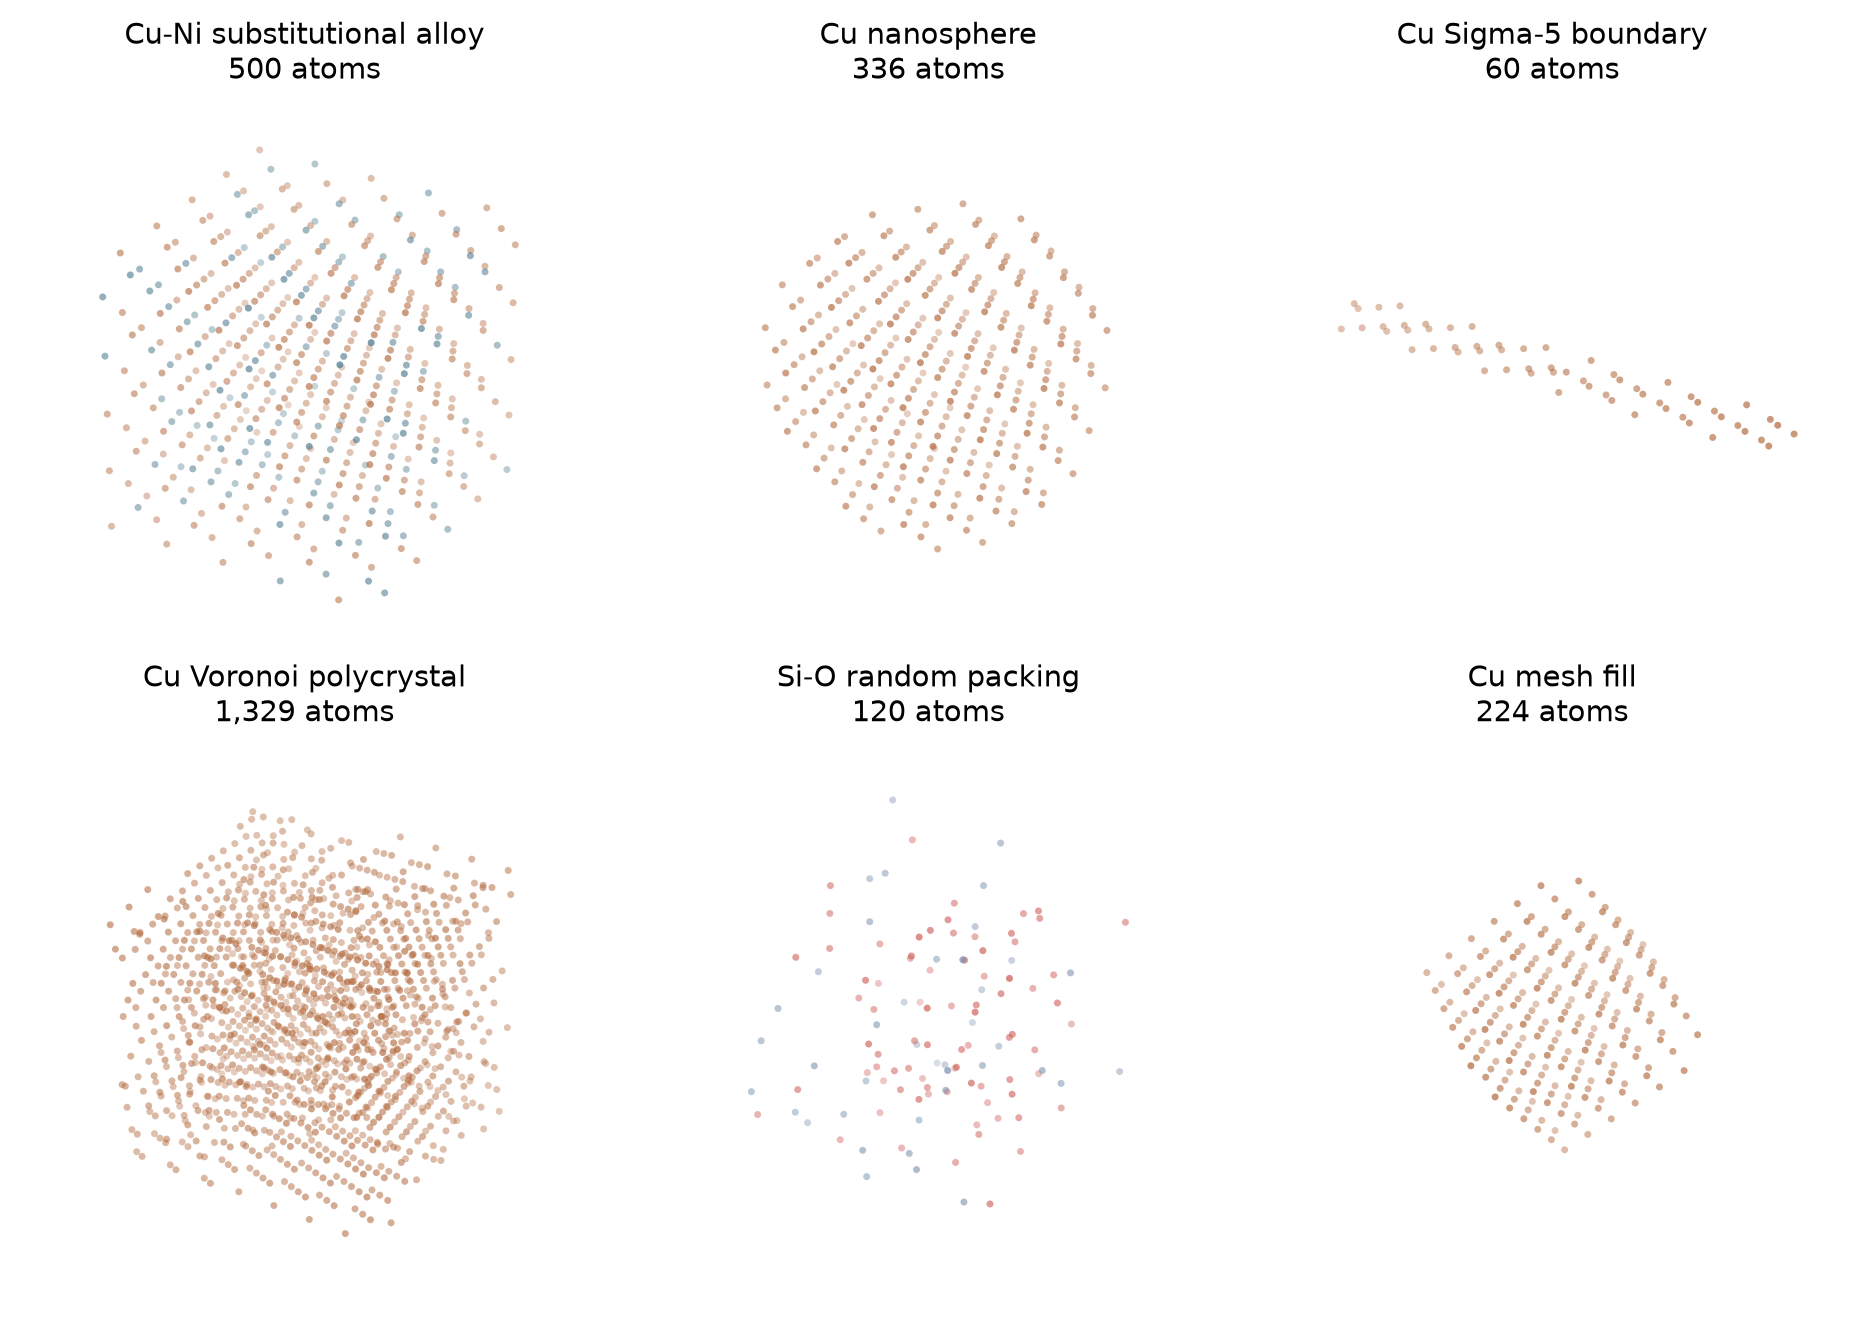
\includegraphics[width=\linewidth]{figures/builder-gallery.png}
\vfill
{\large Documentation edition: 9 September 2026\par}
Application source audited at: \code{e43038c}.\par
Includes reproducible examples, a CHGCAR walkthrough, desktop controls, command-line recipes, and Python integration.
\end{titlepage}
\pagenumbering{roman}
\hypersetup{pageanchor=true}
\chapter*{How to use this manual}
\addcontentsline{toc}{chapter}{How to use this manual}
Start with Chapter~\ref{ch:start} to open a file, construct a crystal, and save a result. Chapters~\ref{ch:builders}--\ref{ch:analysis} explain the structural workflows. Chapters~\ref{ch:electronic}--\ref{ch:reference} cover electronic loading, visualisation, charge redistribution, and the complete electronic operation catalogue. Chapter~\ref{ch:python} provides scripting recipes; the appendices cover installation, reproducibility, and troubleshooting.

Menu names and controls describe the source baseline above and the Windows executable used to prepare the figures. Features controlled by build options are marked explicitly. A source file does not by itself mean a feature is accessible in the desktop menu. Common-neighbour analysis, angular-distribution analysis, and the interface builder are not exposed in the baseline menus; their source interfaces are documented separately. The detailed builder, edit, and display control references supplement the worked examples. Appendix~\ref{ch:coverage} maps the feature families back to source and explains the documentation coverage check.

GUI screenshots are captured from AtomForge. The builder gallery and CHGCAR plots are separately rendered scientific figures calculated from real AtomForge outputs; they are not interface mockups. Example structures are starting configurations, not validated equilibrium structures. The supplied CHGCAR is used to demonstrate the software; its physical system and calculation settings were not independently established.

All paths beginning with \code{examples/} are relative to this manual's folder. Commands use \code{AtomForge} for readability; on Windows substitute the path to \code{AtomForge.exe}. Long command listings may wrap visually; each displayed command is entered as one shell command. Python examples assume the package and native electronic library are available as described in Chapter~\ref{ch:python}.

Chapter~\ref{ch:tutorials} contains 60 illustrated quick tutorials. Each gives a starting input, a short procedure, a result check, and options to try. Use the contents or PDF bookmarks to jump directly to a builder, edit tool, or display option. Seven native nanocrystal examples accompany the shape-cut exercises.

\tableofcontents
\clearpage\pagenumbering{arabic}
\chapter{Getting started}\label{ch:start}
\section{What AtomForge does}
AtomForge is a desktop structure builder and viewer with a native electronic post-processing engine. It constructs atomistic starting configurations, edits positions and cells, renders structures, measures geometric quantities, and processes scalar fields from electronic-structure calculations. It does not run a self-consistent electronic calculation, relax a structure, or predict a formation energy merely by building a model.

The main structure workspace and the electronic dialog maintain different data. Opening a CIF in the main workspace supplies atom positions and a cell. Opening CHGCAR in \ui{Analysis > Electronic Post-processing} supplies a sampled scalar field and imported sites. A structure alone does not contain a charge density; a rendered mesh alone does not contain an electronic wavefunction.

\section{First structure: a copper crystal}
\begin{enumerate}
\item Start the executable. Choose \ui{Build > Bulk Crystal}. Select the cubic crystal system and space group 225.
\item Enter $a=3.61$ \angstrom. Use a Cu site at fractional coordinates $(0,0,0)$ in the asymmetric-unit list. Remove unrelated default sites if present; do not add the three symmetry-equivalent FCC positions yourself.
\item Build the crystal. Inspect the generated structure and its cell. The supplied example \code{examples/cu_fcc.cif} has four Cu atoms in the conventional cubic cell.
\item Close the builder when finished. Use \ui{View > Structure Info} to inspect counts and lattice information.
\item Choose \ui{File > Save As}, browse to your work folder, enter a new filename such as \code{cu_first.cif}, select CIF, and save. Reopen the saved file to check that the cell and species are retained.
\end{enumerate}
If symmetry support is unavailable in a custom build, install/build with spglib or open the supplied expanded CIF instead. The lattice parameter is an example input; select a parameter appropriate to your intended temperature, composition, and calculation method.

\section{Opening, saving, and browsing}
\ui{File > Open} reads a structure into the workspace; \ui{Open Recent} returns to previously used paths. The browser supports directory navigation and file selection. Double-click a directory to enter it, select a file, then use the dialog's opening action. The location field is useful for jumping to a directory; it is not necessary to type the entire file path.

\ui{Save} writes the active structure to its current destination. Use \ui{Save As} to preserve the original and choose a new filename/format. A structure save records supported structural data, not every display setting or electronic intermediate. Save derived electronic grids separately from the electronic dialog. \ui{Close} closes the current structure; \ui{Quit} exits the program. Save valuable edits before closing.

\begin{longtable}{p{.23\linewidth}p{.68\linewidth}}
\toprule Task & Control or shortcut \\ \midrule\endhead
Open a structure & \ui{File > Open}, Ctrl+O. \\
Save active structure & \ui{File > Save}, Ctrl+S. \\
Save a new copy & \ui{File > Save As}, Ctrl+Shift+S. \\
Export rendered image & \ui{File > Export Image}, Ctrl+Alt+S. \\
Close active structure & \ui{File > Close}, Ctrl+W. \\
Undo / redo & \ui{Edit > Undo} and \ui{Edit > Redo}; availability follows the edit history. \\
Electronic analysis & \ui{Analysis > Electronic Post-processing}; available without a structure in the main scene. \\
Appearance controls & \ui{Settings > Atomic Sizes}, \ui{Display Settings}, \ui{Polyhedral Settings}. \\
\bottomrule
\end{longtable}

\section{File types and what survives export}
The desktop uses Open Babel for structure I/O. Its advertised structure extensions include XYZ, CIF, PDB, SDF, MOL, VASP, MOL2, PWI, and GJF. Actual conversion depends on the installed Open Babel plugins. Select a format for the information you need: CIF or VASP for periodic cells, XYZ for simple coordinate interchange, and a molecular format for molecular connectivity where supported.

Plain XYZ does not reliably communicate a periodic lattice to every downstream reader. PDB has format-specific field limits. Format conversions may not preserve custom atom colours, grain identifiers, overlays, or all calculation metadata. Check the exported file in the program that will consume it, especially after transforming a non-orthogonal cell.

Electronic inputs are a separate family: VASP charge/potential/ELF grids, Gaussian Cube, and XSF datagrids. Electronic outputs include XSF, Cube, and VASP grids; CSV tables; and OBJ/PLY isosurface meshes. A CSV profile is a numerical table, while an OBJ surface is geometry. Neither is a replacement for saving the full scalar grid.

\section{Drag and drop}
With the electronic dialog open, drop a supported volumetric file onto the application to load it there. Enable \ui{Drop files as reference} before dropping an operand density. Files arriving during a calculation are queued; wait for the active calculation to finish before interpreting the new field selection. A reference-file drop supplies the second input; it does not subtract anything until you choose and calculate an operation.

Several structure builders accept dropped structures or meshes in their own preview/source regions. Use the visible drop guidance in the active dialog. For an unambiguous workflow, open only the builder you intend to supply and verify the displayed source filename and atom count immediately afterwards.

\section{Orienting and inspecting the main view}
Use the top toolbar's X, Y, Z buttons for Cartesian-axis views and a, b, c for lattice-direction views when a cell is available. The rotation step field and adjacent axis buttons apply a repeatable view rotation. \ui{View > Reset Default View} restores framing; it does not undo atom edits. \ui{Isometric View} and \ui{Orthographic View} change the viewing mode. Use orthographic views when comparing projected distances or alignments.

\ui{Show Atoms} and \ui{Show Bounding Box} control geometry visibility. \ui{Show Element} toggles element labels. \ui{View Structure By} switches available colouring between elements, crystal orientation, and grain-boundary information. Orientation/boundary colouring requires corresponding structure metadata; a plain XYZ file may not contain it.

\ui{View Atoms By} offers balls, ball-and-stick, space-filling, and polyhedral representations when supported by the current state. Bond-like lines and coordination polyhedra are visual/geometric constructs based on neighbourhood criteria; do not infer a quantum-mechanical bond order from their appearance.

\section{A productive project layout}
Create separate folders for input calculations, generated structures, derived fields, tables, and figures. Keep original electronic outputs unchanged. Name derived fields by operation, for example \code{AB_minus_A_minus_B.xsf}, and record the reference weights, grid geometry, selected channel, and units beside numerical results. For publication, retain the actual density difference and quantitative tables as well as the screenshot.

The folder containing this manual follows that pattern on a smaller scale: \code{chapters/} holds editable LaTeX, \code{figures/} holds published illustrations, \code{examples/} holds reusable structures and tables, \code{scripts/} holds regeneration tools, and \code{build/} holds disposable LaTeX/render intermediates.

\chapter{Building atomic structures}\label{ch:builders}
\section{Common builder workflow}
Choose the appropriate command under \ui{Build}, supply a periodic reference where required, set parameters, inspect the preview, and run the build action. Use Load reference in Nanocrystal, CSL, or Polycrystal; Load structure or model in Custom Structure; and Add structure in Merge. These buttons open the shared file picker, while file drops remain available. Read status messages before saving the result. Source previews and generated previews serve different purposes: changing a parameter may update an illustrative preview while the atomic result still needs rebuilding.

Successful Build-menu results open in a new structure tab through the main application's builder callback, preserving the source tab. Merge uses this same new-tab route. Select the generated tab before saving or running another tool. Direct atom edits, Cell Sculptor, Dislocation replacement, and Interstitial insertion update the current structure instead. In the detailed controls below, ``updates the main scene'' refers to the displayed result; it does not mean that every builder overwrites the original tab.

Use modest cells first. Replicating a structure multiplies its atom count; a $10\times10\times10$ replication of a four-atom cell contains 4,000 atoms before cuts. Increasing all three dimensions by two multiplies the workload by eight. Once the geometry is correct, increase size and inspect boundary contacts. A builder does not automatically relax strained bonds or remove every physically undesirable local environment.

\section{Bulk Crystal}
\uishot{bulk-dialog.png}{450bp 175bp 450bp 192bp}{The Bulk Crystal dialog at its initial settings. Change the default H site to Cu and the default lattice parameter to 3.61 Angstrom for the FCC Cu walkthrough. The element button opens a periodic-table picker.}
\textbf{Purpose.} Generate a symmetry-expanded periodic crystal from lattice parameters and asymmetric-unit sites. Inputs are the crystal system, space group, cell dimensions/angles, and element/fractional-coordinate rows.

\textbf{Procedure.} Select one of the seven crystal systems and a compatible space group (1--230). Set independent lattice parameters; check constraints implied by the selected system. Add each crystallographically independent site using an element and direct coordinates. Use the row deletion or clear controls to remove unwanted defaults. Build, inspect the expanded sites, and save a periodic format.

Fractional coordinates are coefficients in $\mathbf r=f_a\mathbf a+f_b\mathbf b+f_c\mathbf c$. They are not distances in \angstrom. Equivalent positions are generated by symmetry; entering a full conventional basis as though every site were independent can duplicate sites. Inspect the final count and short contacts.

\textbf{Worked examples.} FCC Cu with group 225, $a=3.61$ \angstrom, and Cu at $(0,0,0)$ gives four atoms. BCC Fe with group 229, $a=2.87$ \angstrom, and Fe at $(0,0,0)$ gives two. These examples exercise symmetry expansion; they do not determine a thermodynamically optimal lattice parameter.
\begin{lstlisting}
AtomForge --build bulk --system cubic --spacegroup 225 --a 3.61 --atom "Cu 0 0 0" --output cu_fcc.cif
AtomForge --build bulk --system cubic --spacegroup 229 --a 2.87 --atom "Fe 0 0 0" --output fe_bcc.cif
\end{lstlisting}
For lower-symmetry cells, set \code{--b}, \code{--c}, and angles \code{--alpha}, \code{--beta}, \code{--gamma}. Repeat \code{--atom} for independent sites. See \code{--help} for accepted system names.

\section{Substitutional Solid Solution}
\textbf{Purpose.} Assign species to existing lattice sites with requested fractions. This changes chemical labels on a host structure; it does not search for a special quasirandom structure or optimise chemical short-range order.

\textbf{Procedure.} Open a host with enough sites to represent the composition, then choose \ui{Build > Substitutional Solid Solution}. Select the source and species percentages. The GUI uses at\%, with the final row automatically balancing the total to 100\%; the CLI uses fractions summing to one. Choose a fixed seed for reproducibility. Generate the alloy and check the resulting species counts before export. For small hosts, integer atom counts limit the achievable composition.

The example host is a $5\times5\times5$ repetition of conventional FCC Cu: 500 sites. The 70\% Cu / 30\% Ni assignment uses seed 42. Keep the same host atom ordering and seed when reproducing an assignment; changing the host can change which particular sites are substituted.
\begin{lstlisting}
AtomForge --build sss --input cu_host.cif --frac "Cu=0.7,Ni=0.3" --seed 42 --output cu_ni_alloy.cif
\end{lstlisting}
The menu is controlled by \code{ATOMFORGE_ENABLE_SSS_BUILDER}, enabled by default. A seed of zero in the CLI requests a time-dependent seed. After substitution, an external relaxation may be needed to account for atomic size mismatch.

\section{CSL Grain Boundary}
\textbf{Purpose.} Construct a coincidence-site-lattice bicrystal from a compatible cubic periodic reference. A coincidence index $\Sigma$ describes lattice coincidence, not a calculated grain-boundary energy.

\textbf{Procedure.} Load the reference cell in the grain-boundary dialog. Enter a rotation axis $[u\ v\ w]$ and select a supported $\Sigma$ and candidate boundary plane. Set the thickness/repetition of each grain, any gap and vacuum, and an overlap-removal distance. Build and inspect both the interface and periodic cell boundaries. Save the bicrystal and relax it externally before comparing energies.

\textbf{Controls.} The axis is a crystallographic direction. The plane selector chooses from generated candidates. The CLI's \code{--plane} is a zero-based candidate index, not a Miller index. \code{--uca} and \code{--ucb} control stacking repetitions for the two grains. \code{--gap} separates the grains; \code{--vacuum} adds vacuum on each side. \code{--overlap} removes close contacts using a distance in \angstrom; an excessive cutoff can delete desirable interfacial atoms.

\begin{lstlisting}
AtomForge --build gb --input cu_fcc.cif --axis "0 0 1" --sigma 5 --plane 0 --uca 3 --ucb 3 --overlap 1.5 --output cu_sigma5.cif
\end{lstlisting}
This manual's generated example contains 60 atoms. The small thickness makes it a geometry demonstration, not a converged boundary-energy supercell. If \code{--sigma} is omitted, candidate search uses \code{--sigmamax}; specify the exact value when reproducibility matters. \code{--conventional} skips the primitive-cell conversion. Check both lattice compatibility and the selected candidate before interpreting a failed build as a file-format problem.

\section{Nanocrystal: shape cuts}
\textbf{Purpose.} Fill a finite shape with atoms from a periodic crystal. Load a periodic reference, select \ui{Shape Cut}, choose a shape, set dimensions and centre, and use automatic replication unless you need explicit repetition counts. Build the nanocrystal and inspect the output bounding cell.

\begin{longtable}{p{.29\linewidth}p{.62\linewidth}}
\toprule Shape & Main dimensions \\ \midrule\endhead
Sphere & Radius. \\
Ellipsoid & Radii along the three local axes. \\
Box & Half-lengths along the three axes; full side lengths are twice these values. \\
Cylinder & Radius, full height, and cylinder axis. \\
Octahedron & Size parameter for the octahedral cut. \\
Truncated octahedron & Size and truncation parameters. \\
Cuboctahedron & Size parameter for the cuboctahedral cut. \\
\bottomrule
\end{longtable}
\ui{Auto-center from atoms} derives a centre from the reference. Manual centring changes which lattice sites intersect the boundary and can change surface termination and atom count. \ui{Auto-replicate} chooses enough source repetitions for the cut; manual repetitions that are too small truncate the intended object. \ui{Rectangular cell} and vacuum settings provide an enclosing output cell; this does not make a nanoparticle a bulk material.

\begin{lstlisting}
AtomForge --build nano --input cu_fcc.cif --shape sphere --radius 10 --vacuum 5 --output cu_sphere.xyz
\end{lstlisting}
The example contains 336 atoms. Use \code{--rx/--ry/--rz} for ellipsoid radii, \code{--hx/--hy/--hz} for box half-lengths, and \code{--cylradius/--cylheight/--cylaxis} for the cylinder. Explicit source replication uses \code{--repa}, \code{--repb}, and \code{--repc}; zero selects automatic sizing in the CLI.

\section{Nanocrystal: Wulff construction}
Select \ui{Wulff Construction} in the nanocrystal dialog. Add facet families, each with nonzero $(hkl)$ indices and a positive relative surface energy. AtomForge expands families using the reference symmetry, previews the bounding planes, and cuts the periodic crystal by the resulting shape.

\begin{enumerate}
\item Load the periodic reference and check its orientation and symmetry.
\item Add, for example, $(100)$ and $(111)$ families with illustrative energies 1.0 and 0.9. These are demonstration ratios, not material data.
\item Set \ui{Max radius (A)}. The implementation scales plane distances by energy ratios, placing the highest-energy family at this maximum distance. This control is not necessarily the circumscribed vertex radius of the final polyhedron.
\item Inspect the \ui{Wulff Plane View}; family colours help identify the contribution of each family. Remove redundant families or add missing ones as required.
\item Build the atomic nanocrystal. Inspect discrete surface termination separately from the continuous plane preview, then export.
\end{enumerate}
The construction requires a bounded intersection of planes. A family may disappear from the final shape when other planes enclose it. Energy ratios must come from comparable surface calculations if a physical equilibrium-shape interpretation is intended. Atomic discretisation can break an ideal continuous shape's apparent symmetry in a very small particle. The same construction is available through Python \code{af.wulff} and native \code{--build nano --shape wulff}; use repeated \code{--facet "h k l energy"} arguments for the families.

\section{Custom Structure from OBJ/STL}
\textbf{Purpose.} Fill a closed mesh with lattice sites. The mesh is a spatial boundary, not a collection of atoms. Use a watertight OBJ or STL, a periodic atomic reference, a physical scale, and an orientation.

\textbf{Procedure.} Open \ui{Build > Custom Structure}. Load/drop the reference and mesh into their corresponding inputs. Set the mesh scale in \angstrom\ per model unit, then adjust rotation or the Miller-direction alignment. Select enough replication to cover the mesh, set vacuum, and build. Inspect thin features and the atom count; a feature narrower than the lattice spacing may contain no sites.

\begin{lstlisting}
AtomForge --build custom --input cu_fcc.cif --mesh octahedron.obj --scale 12 --vacuum 5 --output cu_mesh.xyz
\end{lstlisting}
The included octahedron has six vertices at the positive and negative unit axes and eight triangular faces. At scale 12 it produces 224 Cu atoms in this example. No Blender installation is required. To use Blender, create a closed mesh, apply the intended object transforms before export, export OBJ/STL, and verify the scale in AtomForge. Inspect for holes, self-intersections, and reversed or inconsistent faces when the fill is missing or unexpected.

The CLI provides \code{--rotx}, \code{--roty}, and \code{--rotz} in degrees. \code{--miller "h k l"} aligns a crystallographic direction with $+Z$ and overrides Euler orientation. A crystallographic direction $[hkl]$ and a plane normal $(hkl)$ differ in a general non-cubic cell; choose the alignment convention deliberately.

\section{Polycrystal}
\textbf{Purpose.} Populate a box with grains cut by a Voronoi partition. Inputs include a periodic reference, box dimensions, grain count, random seed, and optional orientations. The construction creates geometric grain boundaries; it does not optimise their energies.

\textbf{Procedure.} Load a reference, enter box lengths and grain count, set the seed, and choose orientations or random assignment. Generate, inspect the grain sizes and contacts, and save. Use orientation colouring when the output retains orientation metadata. Reopening a format that lacks grain metadata can preserve atoms while losing those colours.

\begin{lstlisting}
AtomForge --build poly --input cu_fcc.cif --sizex 25 --sizey 25 --sizez 25 --grains 4 --seed 7 --output cu_polycrystal.cif
\end{lstlisting}
This example contains 1,329 atoms. The CLI accepts repeated \code{--euler "phi1 Phi phi2"} triplets in Bunge convention, one per grain; unspecified orientations are random. Use the same seed, dimensions, reference, and ordering to reproduce a sample. Increase the box relative to grain count when grains become too small to have a meaningful crystalline interior.

\section{Amorphous Structure}
\textbf{Purpose.} Produce a random packing subject to distance constraints. Specify elements and counts, a mass density or explicit box, pair-distance constraints, and a seed. This is an initial configuration generator; random packing alone does not establish a realistic glass network.

\textbf{Procedure.} Add the required species/count rows. Set density in $\mathrm{g\,cm^{-3}}$ or explicit box dimensions. Check the minimum separation settings; overly strict cutoffs at a high density can make placement impossible. Set a fixed seed, generate, and inspect the reported inserted count and any placement failure. Relax or equilibrate the configuration with a suitable external method before structural or energetic claims.

\begin{lstlisting}
AtomForge --build amorphous --element "Si 40" --element "O 80" --density 1.5 --seed 7 --output sio2_pack.xyz
\end{lstlisting}
The example has 120 atoms with a 1:2 Si:O ratio. The deliberately low packing density is useful for demonstrating construction and is not a claim about silica's equilibrium density. \code{--boxa/--boxb/--boxc} override density-derived dimensions. \code{--mindist "Z1 Z2 distance"} adds a pair constraint using atomic numbers; \code{--covtol} controls the covalent-radius fallback; \code{--attempts} bounds placement attempts. If placement fails, examine the geometry and constraints before merely raising the attempt limit.

\section{Optional and unavailable builder menus}
The stacking-fault builder is compiled into the desktop menu only with \code{ATOMFORGE_ENABLE_SFE_BUILDER=ON}; the default is OFF. Its purpose is to construct faulted configurations, not to calculate a stacking-fault energy. In an enabled build, open \ui{Build > Stacking Faults}, supply a reference with \ui{Use Current Scene} or the source workflow, and click \ui{Detect Structure}. Select a supported Plane, choose \ui{Smallest Unit Cell} or \ui{Orthogonal Cell}, and set Layers (2--96). Click \ui{Generate Sequence}, use the Structure slider to inspect its members, and choose \ui{Use Selected Structure} to adopt one. \ui{Export All Structures} writes the sequence to the specified Folder/Subfolder; \ui{Use Source Folder} supplies a convenient base when available. Validate the stacking geometry and calculate energies externally. This optional path was inspected in source but not enabled in the screenshot executable.

The interface-builder dialog has a drawing call but no current main-menu entry to open it. Its source/API capabilities are described in Appendix~\ref{ch:coverage}. Use the exposed merge/transform workflows for manual assembly in the current executable.

\section{Worked study: compare bulk and finite Cu environments}
This exercise connects building, file inspection, and structural analysis. It uses only generated structures and does not require an electronic calculation.
\begin{enumerate}
\item Open \code{examples/cu_fcc.cif}. Inspect its four sites and cubic cell. The cell edge is 3.61 \angstrom. Save a working copy before changing it.
\item Open the supplied \code{cu_host.cif}, or create it by repeating the conventional cell $5\times5\times5$ through Python. It contains 500 atoms. Use this larger periodic host for bulk neighbour statistics.
\item Open \code{cu_sphere.xyz} separately. It contains 336 atoms from the same reference lattice, cut at radius 10 \angstrom. Rotate it and inspect surface sites. The smaller count is caused by the finite shape, not by a different crystal symmetry.
\item Run RDF on the periodic host with Cu as both species, PBC enabled, and no smoothing. Check the first-neighbour peak near 2.553 \angstrom. Begin with a cutoff that is comfortably smaller than the box dimensions.
\item Run RDF on the finite sphere with PBC disabled. Compare raw counts and cumulative coordination before comparing normalised curves: the particle has surface atoms with incomplete neighbour shells and its enclosing vacuum does not define a bulk atomic density.
\item Open \code{cu_ni_alloy.cif}. Verify 350 Cu and 150 Ni atoms, then inspect Cu--Cu and Cu--Ni partial distributions and the SRO table. The unrelaxed substitution changes labels while retaining ideal host positions; it cannot demonstrate size-mismatch relaxation.
\end{enumerate}
Keep the source filenames, cutoffs, species choices, PBC setting, bin count, and smoothing with each plot. If the bulk nearest-neighbour peak moves unexpectedly, first check lattice scaling and units. If coordination falls at the surface of the sphere, inspect its geometric boundary before treating the change as disorder. If the alloy has nonzero measured SRO, compare seeds and finite-size effects before interpreting it as evidence of an energetic ordering preference.

This comparison illustrates why a common visual appearance does not guarantee comparable statistics. The bulk, particle, and alloy answer different questions even though they originate from the same Cu cell. Choose analysis settings according to the geometry and composition of each saved structure.

\section{Builder control reference}\label{sec:builder-controls}
The following reference supplements the worked examples with the controls that are easy to miss in a scrolled dialog. Open the appropriate Build command, then scroll its settings panel independently of its preview. Drag numeric fields for exploration; Ctrl+click an ImGui drag field to enter a precise value. Check the result after rebuilding: changing a parameter does not necessarily regenerate the atomic structure.

\subsection{Bulk Crystal: symmetry, lattice, and site editor}
\begin{description}
\item[Crystal system.] Select the system first. This restricts the space-group list and determines which lattice parameters can be entered. Changing system can change the valid group selection, so recheck the group before building.
\item[Space group.] Choose the numbered group in the filtered list. The asymmetric-unit sites are expanded using this symmetry. A site on a special position has fewer distinct equivalents than a general site.
\item[Lattice parameters.] Lengths are in \angstrom; angles are degrees. Triclinic exposes all six values. Monoclinic exposes $a,b,c,\beta$ with $\alpha=\gamma=90^\circ$. Orthorhombic exposes $a,b,c$ with right angles. Tetragonal exposes $a,c$ with $b=a$. Trigonal uses the hexagonal setting, as does Hexagonal: $b=a$, $\alpha=\beta=90^\circ$, $\gamma=120^\circ$. Cubic exposes $a$, with $b=c=a$ and right angles. Do not enter rhombohedral primitive-cell parameters into the trigonal hexagonal-setting controls.
\item[\normalfont\ui{+ Add}, \ui{Clear}, \ui{Delete}.] Add creates an independent site row. Clear empties the asymmetric-unit list; Delete removes only its row. A nonempty valid site list is required for a useful build.
\item[Site coordinates.] The three values are direct coordinates, not Cartesian distances. Enter one representative of each independent site. Negative or out-of-cell input should be checked in the symmetry-expanded result rather than treated as an extra supercell site.
\item[Element button and Apply Element.] Click the row's element button, choose an element in the periodic table, and apply it to that row. This selects chemical identity; it does not set oxidation state, occupancy, magnetic moment, or a pseudopotential.
\item[Build and Close.] Build generates the expanded crystal and updates the main scene when successful. Read the status and inspect atom count. Close dismisses the dialog; save the generated scene with File > Save As.
\end{description}
\textbf{Diagnostic example.} For NaCl, use group 225 and independent Na $(0,0,0)$ and Cl $(1/2,1/2,1/2)$ sites. The conventional cell should contain four of each species. Use an appropriate lattice parameter for the intended study. If the count is wrong, check group, coordinates, and duplicated independent rows before expanding the cell.

\subsection{Substitutional Solid Solution: every composition control}
\begin{description}
\item[Source / Use Current Scene.] Load a host or copy the current scene into the source preview. Composition controls become useful after a nonempty host is present. The host supplies the sites to relabel.
\item[Element rows.] Click an element symbol to select a species. \ui{+ Add Element} adds another species; the row's X removes it when more than one row exists. Avoid duplicate species rows when specifying a composition.
\item[at\%.] The GUI uses atomic percentages from 0 to 100. The \emph{last row is a read-only remainder}: its percentage is 100 minus the preceding rows. To make Cu--Ni 70:30, put Cu first and Ni last, then enter 70 for Cu. To make a ternary 50:30:20, enter 50 and 30 in the first two rows. The last row becomes 20. Recheck the whole table after adding or removing a row.
\item[Atom count.] The displayed count is a consequence of the percentage and host size, not an independent composition input. Integer site allocation limits resolution to approximately $100/N$ percentage points for $N$ sites.
\item[RNG seed.] A positive fixed integer makes the site assignment reproducible for the same input ordering. Zero selects a random/time-dependent assignment; negative input is clamped to zero.
\item[Build Solid Solution.] Apply the assignment, then verify counts in Structure Info. The CLI equivalent uses fractions such as \code{Cu=0.7,Ni=0.3}; do not paste GUI percentages into \code{--frac}.
\end{description}
\textbf{If a percentage cannot be edited:} first check whether it is the last row. This is the balancing row, not a disabled builder. Change the preceding rows or their ordering/composition instead.

\subsection{CSL Grain Boundary: search, geometry, and result}
\begin{description}
\item[{Rotation axis $[uvw]$.}] Enter a nonzero integer direction for the cubic reference. Changing the axis requires a new candidate search.
\item[Maximum Sigma and Find.] The maximum bounds the candidate search; Find populates the Sigma selector. A larger bound expands the search, not the physical sample size.
\item[Sigma and GB plane.] Select a coincidence candidate, then a boundary plane from the generated choices. The plane selector contains candidate planes; the CLI index 0, 1, or 2 selects one of these choices. It is not the value of $h$, $k$, or $l$.
\item[Grain A (uc), Grain B (uc).] Set repetitions used to thicken each grain along the stacking construction. Use both controls to study symmetric or unequal thicknesses. These are integer cell repetitions, not distances in \angstrom.
\item[Vacuum (A), Gap (A).] Vacuum adds the specified outside spacing in the construction; Gap separates the stacked grains. Both alter geometry. Neither is a relaxation or a search over rigid translations.
\item[Overlap distance (A).] Remove interfacial close contacts within the chosen cutoff. Inspect the removed-atom count and resulting stoichiometry. Set a conservative cutoff and compare before raising it.
\item[Conventional cell.] Retain the conventional construction when enabled; otherwise the builder attempts its primitive grain-boundary cell reduction. This can change the final cell representation and atom count.
\item[Build and result summary.] Build updates the main structure. Record Sigma, misorientation angle, boundary plane/type, axis, CSL matrix, grain repetitions, gap, vacuum, input/generated counts, and removed overlaps. These identify the geometry more precisely than a filename containing only Sigma.
\end{description}
\textbf{Troubleshooting.} If Find produces no appropriate candidate, verify the axis and cubic reference first. If Build produces too few atoms, compare overlap removal and primitive reduction before changing the reference. This dialog has no general rigid-translation energy-search control.

\subsection{Nanocrystal: shape parameters and shared output controls}
All shape dimensions below refer to the local shape coordinates about the chosen centre. For relative coordinates $(x,y,z)$, the implemented cuts are:
\begin{longtable}{p{.24\linewidth}p{.67\linewidth}}
\toprule Shape & Parameters and membership rule \\ \midrule\endhead
Sphere & Radius $R$: $x^2+y^2+z^2\leq R^2$. \\
Ellipsoid & Semi-axis $a,b,c$: $(x/a)^2+(y/b)^2+(z/c)^2\leq1$. \\
Box & Half-size X/Y/Z: each absolute coordinate is bounded by its half-size. \\
Cylinder & Radius and full Height, with Axis X/Y/Z selecting the longitudinal direction. \\
Octahedron & Octahedron radius $R$: $|x|+|y|+|z|\leq R$. \\
Truncated octahedron & Octahedron R and Truncation R: both the octahedron bound and $\max(|x|,|y|,|z|)\leq R_t$ apply. \\
Cuboctahedron & The currently named cut uses the three bounds $|x|+|y|\leq R$, $|y|+|z|\leq R$, $|x|+|z|\leq R$. Use this implemented definition when reproducing its geometry. \\
\bottomrule
\end{longtable}
\begin{description}
\item[Auto-center from atoms / Center X,Y,Z.] Automatic centring follows the reference atoms. Disable it to specify a Cartesian centre in \angstrom. A shift smaller than a lattice spacing can still change the surface termination.
\item[Auto-replicate / Rep a,b,c.] Automatic mode sizes the source coverage. Manual mode uses the three integer repetitions; increase all necessary directions if the shape is clipped by insufficient source coverage.
\item[Rectangular cell / Vacuum.] Choose a rectangular enclosing output cell where needed and add the requested surrounding vacuum in \angstrom. Inspect the saved cell in a periodic format; a plain XYZ consumer may ignore the cell.
\item[Wulff family editor.] Each row has $h,k,l$, a positive relative energy, a display colour, and Remove. Add Family adds a row. The last remaining family cannot simply be removed with the row control. Add enough symmetry-related constraints to bound the shape; zero indices or nonpositive energies are not meaningful input.
\item[Max radius and plane preview.] Max radius sets the distance of the highest-energy family, with others proportional to energy. Family colour changes the plane preview, not surface energy. Build the atoms again after changing family energies or geometry.
\end{description}

\subsection{Custom Structure: reference, mesh, and orientation}
\begin{description}
\item[Reference source, Clear, Use Current Scene.] Load a periodic reference or copy the current scene. Clear removes that source. The separate mesh Clear control clears the mesh, not the atomic reference.
\item[OBJ/STL source and Scale.] Load the enclosing mesh and enter \angstrom\ per model unit. A unit-radius mesh at scale 12 represents a 12 \angstrom\ radius along the corresponding model axes. Verify the preview's physical extent before building.
\item[Auto-center / Center X,Y,Z.] Automatic centring derives placement from the reference; manual values specify the centre. Inspect reference and mesh together to avoid filling an unintended region.
\item[Apply crystal orientation.] Enables the orientation controls. The current radio labels \ui{1} and \ui{2} select Euler-angle and Miller-direction modes respectively. In mode 1 enter Rot X/Y/Z in degrees. In mode 2 enter $h,k,l$ for direction alignment. This rotates the crystal filling relative to the mesh; orbiting the preview camera does not substitute for it.
\item[Auto-replicate / Rep a,b,c.] Ensure enough periodic sites to cover the whole mesh. Manual undercoverage can look like a broken mesh cut.
\item[Output enclosure.] Set rectangular output cell and Vacuum configure the enclosure and surrounding spacing. These do not repair holes in the mesh or close a non-watertight boundary.
\item[Build Fill / Close.] Build Fill generates the atomic product from both inputs. Verify the count and thin sections before saving. Close dismisses the builder.
\end{description}

\subsection{Polycrystal: dimensions, randomisation, and individual grains}
\begin{description}
\item[Reference and X/Y/Z.] Supply a periodic reference and the three target box lengths in \angstrom. The dimensions define the total specimen, not the size of every grain.
\item[Number of grains.] Sets the number of Voronoi seeds/grains. Increasing it at fixed volume reduces typical grain size. Check that grains contain sufficient interior sites for the intended analysis.
\item[Seed.] Keep a fixed seed to reproduce the stochastic construction along with all other inputs.
\item[All Random.] Generate all orientations randomly.
\item[All Specified.] Edit the Bunge Euler triplet $(\phi_1,\Phi,\phi_2)$ in degrees for every grain. The table grows with the grain count and may require scrolling.
\item[Partial (specify some, rest random).] Enter \ui{Grain \#} using the GUI's one-based numbering, then \ui{Add Grain Orientation}. Duplicate grain entries are not added. Edit that grain's three angles; X removes the explicit override so the grain returns to random assignment. Unspecified grains remain random.
\item[Build / Close.] Build the sample and inspect orientation colouring and boundary contacts. Preserve the generated \code{.atomforge-ipf} sidecar beside an associated exported structure when retaining orientation metadata. Close leaves the generated scene available for saving.
\end{description}

\subsection{Amorphous Structure: composition and packing constraints}
\begin{description}
\item[Element and Count rows.] Choose each species with its element button, enter its integer atom count, and use X or Add Element to change the list. Check the total and formula before choosing density.
\item[Auto from target density.] Enter mass density in $\mathrm{g\,cm^{-3}}$. The builder estimates a cubic box using the total atomic mass. The displayed side length includes the Cell scale factor.
\item[Manual dimensions.] Enter $a,b,c$ in \angstrom\ to set box lengths explicitly. This mode replaces density-derived sizing.
\item[Cell scale factor.] Multiplies box lengths before packing. Scaling lengths by $s$ multiplies volume by $s^3$, so a density-derived box has effective density $\rho/s^3$. For example, $s=1.1$ yields approximately $0.751\rho$. The target-density label alone therefore does not describe the final density when scaling is enabled.
\item[Periodic boundary conditions (attach unit cell).] Controls whether the output carries the unit cell. The current packing implementation checks minimum-image separations across the box even when this output-cell option is off. Retain a cell-capable format for subsequent periodic analysis and inspect cross-boundary contacts.
\item[Advanced Settings.] Expand this section to reveal placement controls and the element-pair table. These are part of the builder, not separate menu commands.
\item[Covalent radius tolerance.] The fallback minimum separation is $(r_i^{\rm cov}+r_j^{\rm cov})t$. Smaller $t$ permits closer contacts; it does not calculate bonding.
\item[RNG seed (0 = time).] Use a nonzero integer to repeat the random placement. Zero requests a time-dependent seed.
\item[Max attempts per atom.] Bounds trials for each requested atom. Raising it increases work but cannot guarantee a feasible packing.
\item[Element-pair minimum distances.] Check a pair's row to enable its explicit minimum distance in \angstrom. An unchecked row uses the displayed covalent-radius fallback. Apply different overrides only when their chemical/geometrical interpretation is intentional.
\item[Build and status.] Compare requested and inserted counts. If atoms are skipped or placement fails, increase box size, reduce a conflicting minimum distance, or revise composition before simply increasing attempts. Save the final structure and record the actual density.
\end{description}

\subsection{Optional Stacking Faults: sequence and export controls}
In a build with the SFE option enabled, \ui{Detect Structure} classifies the reference and populates supported plane choices. Select the Plane and the Smallest Unit Cell or Orthogonal Cell mode, then set Layers. \ui{Interval} controls the increment of the displacement sequence; \ui{Max Displacement} controls its maximum displacement factor. These are sequence-construction parameters, not energies in eV. Smaller intervals create more configurations and more export files.

Choose \ui{Generate Sequence} after changing these inputs. The \ui{Structure} slider selects a zero-based member of the generated sequence for preview. \ui{Use Selected Structure} replaces the main scene with that member. For batch output, enter the base \ui{Folder} and \ui{Subfolder}, or use \ui{Use Source Folder} where available, then \ui{Export All Structures}. Unlike the current general file picker, this optional source implementation still contains text folder fields. Record each member's displacement alongside its externally calculated energy before constructing a stacking-fault-energy curve. This optional dialog was audited in source, not enabled for the manual screenshots.

\chapter{Editing, assembly, and defects}\label{ch:editing}
\section{Selection and edit history}
Click an atom in the main scene to inspect/select it. Left-drag orbits the camera; right-drag normally pans. When \ui{Edit > Box Select} is active, right-drag draws a selection rectangle instead. \ui{Lasso Select} uses a right-drag path for a more irregular projected region. Selection is based on the current projection, so inspect the result from another direction before acting on a dense or overlapping set of atoms.

Open \ui{Edit > Edit Structure} to work with the atom table. Use \ui{Undo} and \ui{Redo} where enabled, but retain saved checkpoints before substantial assembly or defect-generation operations. A camera reset changes only the view and does not restore a previous structure.

Ctrl+left-click adds/removes an atom from the selection. Ctrl+A selects all; Ctrl+D or Escape clears selection. Delete removes selected atoms, and right-click opens the selection context menu. Ctrl+Z undoes; Ctrl+Y or Ctrl+Shift+Z redoes. Use these shortcuts in the main workspace with no text-entry field focused.

\section{Edit Structure: atoms and cell}
The editor exposes cell vectors when a cell is present and an atom table with element and coordinate editing. \ui{Position Mode} switches between \ui{Cartesian} and \ui{Direct}. Cartesian coordinates are in \angstrom; direct coordinates are fractional lattice coefficients. Direct editing is disabled without a unit cell.

\begin{enumerate}
\item Open the source structure and save a working copy.
\item Choose \ui{Edit > Edit Structure}. Confirm the coordinate mode before typing a position.
\item Select a row to edit the desired atom. Use the element selection and \ui{Apply Element} controls for species changes.
\item Use \ui{Add Atom} to create a new row, then immediately set its element and position. The initial atom is H at the origin; leaving it there may create an overlap.
\item Inspect changed positions and atom counts in the viewport and information dialog. Save the revised structure under a descriptive name.
\end{enumerate}
Cell-vector edits define the simulation cell. Do not assume that typing a new box automatically performs the same operation as a homogeneous strain or a supercell construction. Check the resulting atom coordinates and boundary relationships. Use the integer transformation tool for deliberate periodic supercells.

\section{Transform Structure}
\ui{Edit > Transform Structure} accepts three rows of integer coefficients. It is available for a structure with a unit cell. Begin with a diagonal transformation to establish the convention: $(2,0,0)$, $(0,2,0)$, $(0,0,2)$ creates a $2\times2\times2$ periodic enlargement. For conventional FCC Cu this should contain 32 atoms when the reference contains four.

Enter the matrix, choose \ui{Apply}, and inspect the resulting lattice vectors, volume, and atom count. \ui{Cancel} discards the pending matrix. Non-diagonal matrices define combinations of lattice directions and are useful for rotated supercells. The matrix must be nonsingular; a zero determinant cannot define a three-dimensional cell. For valid integer supercells, the determinant magnitude gives the ideal volume/atom-count multiplier before additional cuts or deduplication. Verify this count rather than assuming any arbitrary matrix represents the intended orientation.

\section{Merge Structures}
\textbf{Purpose.} Assemble several structures in an interactive preview. Open \ui{Edit > Merge Structures}, load/drop the components, and select one component at a time. Its transform and gizmo controls translate or rotate that component; camera movement changes the view of the entire assembly.

\begin{enumerate}
\item Prepare and save each input independently with consistent length units.
\item Add the inputs to the merge dialog. Check each component's identity before moving it.
\item Select a component and use the visible gizmo handles to position/orient it. Inspect from at least two directions; two objects that appear separated in one projection can intersect in three dimensions.
\item Toggle \ui{Show Bounding Box} to inspect the enclosure. Use \ui{Delete Selected} to remove an unwanted component from the assembly, or \ui{Clear All} to start the assembly again.
\item Choose \ui{Merge Structures}, inspect the resulting scene, and save a new structure.
\end{enumerate}
Merging is geometric assembly. It does not find a low-strain epitaxial match, remove all close contacts, or determine a chemically correct interface termination. Inspect separations, stoichiometry, cell conventions, and periodic contacts before using the merged structure in a simulation.

\section{Cell Sculptor: supercells and cutting slabs}
\ui{Edit > Cell Sculptor} combines a periodic source, supercell repetitions, and cutting planes/slabs. Use \ui{Use Scene} to obtain the current structure or supply a source through the dialog's load/drop workflow. The source and result previews help distinguish the uncut periodic model from the generated product.

\textbf{Procedure.} Set the supercell repetitions first. Add a cutting slab, enter nonzero Miller indices, choose periodic or distance-based limits, and inspect the plane preview. Add further slabs when the desired region needs multiple constraints. Set the outside-atom opacity to make excluded atoms less prominent, then choose \ui{Generate}. Save the resulting atomic structure only after checking which side of each boundary was retained.

In periodic slab mode, \ui{Start} identifies the starting plane and \ui{N} controls the number of structural repeats/layers along the slab normal. The displayed spacing derives from the lattice. A crystallographic repeat interval can include several chemically distinct atomic layers; do not equate \ui{N} blindly with the number of visible atomic sheets. Distance-based limits use \angstrom\ and are useful for a finite cut without an integer repeat interpretation.

For a lattice with reciprocal vectors defined without $2\pi$,
\[
\mathbf a^*\cdot\mathbf a=1,\quad
\mathbf a^*\cdot\mathbf b=\mathbf a^*\cdot\mathbf c=0,
\qquad d_{hkl}=\frac{1}{|h\mathbf a^*+k\mathbf b^*+l\mathbf c^*|}.
\]
The normal to a plane is a reciprocal-space combination. For a skew cell it is generally not the same Cartesian direction as $h\mathbf a+k\mathbf b+l\mathbf c$. Use the preview to confirm the orientation before generating a slab. Geometric cutting can create polar surfaces or nonstoichiometric terminations; choose terminations according to the intended study.

\section{Insert Dislocation}
\textbf{Purpose.} Apply a continuum-style displacement construction to a structure. Open \ui{Edit > Insert Dislocation}, use the current scene or load a reference, and use \ui{Detect Lattice} to inspect the lattice classification before choosing directions.

\textbf{Character and region.} Choose Edge, Screw, or Mixed character. Available region shapes are Half-plane, Cylinder, Sphere, Ellipsoid, and Freeform 2D. These control the construction region. They do not by themselves certify a particular relaxed dislocation-core structure or a stable physical loop.

\begin{enumerate}
\item Choose a sufficiently large reference and a fixed cell geometry.
\item Enable \ui{Auto lattice vectors} for inferred directions, or enter the slip-plane indices, Burgers direction, and line direction manually. Use crystallographically compatible, nonzero directions.
\item Locate the line using a fractional point when convenient, or the Cartesian position/offset controls. Confirm its position in the preview.
\item Set Burgers-vector scale, Poisson ratio, core radius, cutoff, and line extent. For Mixed character, set the mixed angle. Supply the selected shape's dimensions or the Freeform 2D points.
\item Choose \ui{Generate Dislocation}. Inspect RMS and maximum displacement and the displaced structure.
\item Use \ui{Replace Main Scene} to adopt the generated result, then save a new file.
\end{enumerate}
The core radius regularises the near-core field; it is a modelling parameter, not an experimentally measured core width inferred by AtomForge. The continuum approximation is least reliable near the core. Periodic boundary conditions can require compatible dislocation arrangements; an isolated displacement construction in a periodic box may create artificial long-range strain. Relax and validate with an appropriate external model.

\section{Add Interstitial Atoms and detect voids}
\textbf{Purpose.} Find geometric void candidates and place chosen atoms in selected subsets. Open \ui{Edit > Add Interstitial Atoms}, select \ui{Use Current Scene} or provide a host, and run \ui{Detect Voids}.

\textbf{Detection controls.} \ui{Grid} controls the search resolution (8--30 in the current UI); \ui{Max Voids} limits candidates. Higher resolution can find different candidates at higher cost. Use the void-type filters to include the desired coordination geometries. \ui{Select All Types} and \ui{Clear All Types} manage those filters. \ui{Show Void Polyhedra in Scene} helps relate candidate centres to their coordinating atoms.

\textbf{Placement modes.}
\begin{description}
\item[Random distribution] Choose a percentage or atom count and a seed. The percentage refers to eligible candidate sites, not automatically to the final atomic composition.
\item[Inside OBJ/STL mesh region] Load a mesh region and transform it with Translate (T), Rotate (R), and Scale (S). Inspect the mesh relative to the host; \ui{Reset Transform} restores its transform. Choose a target percentage/count among eligible sites in that region.
\item[Manual (selected voids only)] Select candidate centres in the preview and check the displayed selected-centre count. The selected subset determines placement.
\end{description}
Use \ui{Select Element} to choose the inserted species, then \ui{Apply Interstitials}. Inspect the atom-count change and nearest-neighbour separations before saving. A void is a geometric candidate, not a calculated formation-energy minimum. Site preference, charge state, local relaxation, and solubility require separate physical calculations.

\section{Checking an edited model}
Before exporting a simulation input, check species counts, cell vectors, boundary contacts, minimum interatomic distances, and the intended periodicity. For nanoparticles and slabs, check vacuum in every relevant direction. For substitutions and defects, compare composition before and after the edit. Save both the starting model and the exact edited model used for later calculations.

\section{Detailed edit controls and application points}\label{sec:edit-controls}
The main distinction between edit tools is when and where they change structure data. Table edits change the current structure immediately; Dislocation has a separate preview-generation and replacement step; Merge opens its committed result in a new tab; Interstitials commits to the current structure; Cell Sculptor commits to the current structure and closes on a valid Generate. Save an input checkpoint before a sequence of operations.

\subsection{Atom selection and the right-click menu}
\begin{description}
\item[Box Select Mode / Lasso Select Mode.] The two Edit menu modes are mutually exclusive. Their projected selection includes atoms along the viewing direction. Change the view to check selection depth before deletion or substitution.
\item[Substitute Atom.] Select the intended atoms, open the context menu, choose this action and an element, then apply. It changes the species of the selected underlying atoms. A displayed periodic image maps back to its base atom; selecting an image does not create an independent species assignment for that image.
\item[Insert Atom at Midpoint.] Requires at least two selected atoms. Choose the new element and apply. With two selections, the new position is their displayed Cartesian midpoint. With more than two, the implementation uses the centroid of all selected displayed positions, $\mathbf r_{\rm new}=N^{-1}\sum_i\mathbf r_i$. It is not a periodic minimum-image midpoint. Select the appropriate images if atoms straddle a boundary.
\item[Measure Distance / Measure Angle / Atom Info.] Context actions require exactly two, three, or one selected atom respectively. Choose the middle/vertex atom deliberately for angle measurements and inspect the overlay.
\item[Delete / Deselect.] Delete removes selected base atoms from the structure; Deselect only clears selection. The context menu can be unavailable when large-scene CPU picking caches are disabled. A visible atom rendering alone does not guarantee that all interactive per-atom actions are enabled.
\end{description}
\textbf{Example.} Select two neighbouring Cu sites and insert H at their midpoint, then measure H--Cu distances and inspect for overlaps. This creates a geometric trial position, not a validated interstitial site. For systematic void-based insertion, use Add Interstitial Atoms below.

\subsection{Edit Structure: exact effects of the table}
\begin{description}
\item[Cell vectors a, b, c.] Each row contains three Cartesian components in \angstrom. Editing a vector changes the cell and display buffers, but does not rescale atom positions. To double a periodic crystal with replicated sites, use Transform Structure instead of doubling a vector here.
\item[Position Mode: Cartesian / Direct.] Cartesian fields edit positions in \angstrom. Direct fields convert fractional coefficients through the current cell. Direct mode is unavailable without a cell. Changing mode changes coordinate representation; it does not itself move the atom.
\item[Atom position rows.] Edit the three coordinates in the chosen mode. Table edits take effect in the active scene; there is no separate global Apply for all coordinate changes.
\item[Element button / Apply Element.] Choose a species in the periodic-table popup and apply it to the row being edited. This is a row-specific edit; use the context-menu substitution for a selected group.
\item[Add Atom / Delete.] Add Atom starts an H atom at the origin. Set its species and coordinates immediately. Delete removes the corresponding row. Atom numbering can change after row removal, so recheck any saved index-based filter or selection.
\end{description}
\textbf{Cell-edit check.} Record one atom's Cartesian position, change only a lattice-vector component, then read the atom position again. Its Cartesian coordinates remain unchanged while its fractional coordinates generally change. This is why direct cell editing must not be mistaken for applying a homogeneous strain.

\subsection{Transform Structure: matrix entry and validation}
Each of the three displayed rows is an integer vector. Begin with the identity matrix to understand the entry layout, then set the requested transformation and Apply. A diagonal $(2,1,1)$ enlargement means diagonal entries 2, 1, 1 and all off-diagonal entries zero. It should double an ideal periodic atom count and volume. Entering three copies of the vector $(2,1,1)$ instead would make the matrix singular.

For a non-diagonal transform, inspect the resulting cell vectors rather than inferring orientation solely from the matrix on screen. Cancel discards the pending transform. The command is disabled without a unit cell. A negative determinant changes handedness; zero determinant is invalid. Save the transformed result separately before performing a finite cut.

\subsection{Merge Structures: component transforms and output cell}
\begin{description}
\item[Load/drop components.] Add each source to the component list. Select its row or preview object before changing its transform. The component label identifies which input the numeric controls affect.
\item[Pos (A).] The three values translate the selected component in Cartesian \angstrom. Use these fields for reproducible offsets after coarse gizmo placement.
\item[Rot (deg).] Three rotation values orient the selected component. The preview reflects its component transform; orbiting the camera changes the view of all components together.
\item[Gizmo handles.] Drag translation/rotation handles of the selected component. Inspect from another camera direction to distinguish a transform from projection overlap.
\item[Reset and removal actions.] Reset restores the selected component's transform. Remove and Delete Selected remove a component from the assembly. Clear All clears the assembly inputs. These actions do not delete the input files on disk.
\item[Show Bounding Box.] Displays the assembly enclosure for inspection. This overlay is not a new periodic lattice definition.
\item[Merge Structures.] Commits transformed atoms to the main scene. The current implementation explicitly clears the unit cell and grain metadata. The result is a nonperiodic assembly, even if both inputs were periodic. Cell-dependent tools will consequently be unavailable until a valid cell is supplied through an appropriate workflow. Save a coordinate format when no periodic cell is intended.
\end{description}
\textbf{Example.} Add two copies of the supplied Cu particle, translate one along X by more than the particle diameter, merge, and inspect the atom count. Reduce the offset only after checking the nearest interparticle contacts. Merge does not automatically remove overlaps.

\subsection{Cell Sculptor: closing a region and defining each slab}
\begin{description}
\item[Use Scene / source / Clear.] Supply a periodic atomic source. Clear removes it from the tool. Set the source before defining crystallographic cuts.
\item[Supercell $n_x,n_y,n_z$.] Set positive repetition counts (GUI range 1--30) to supply enough source sites. These counts describe available atomic coverage; the slabs determine retained geometry.
\item[Slab $h,k,l$.] Each slab is the intersection of two parallel half-spaces with reciprocal-lattice normal $h\mathbf a^*+k\mathbf b^*+l\mathbf c^*$. The zero triplet is invalid. Edit the existing row or use the new-slab controls and Add Slab.
\item[Periodic / Start / N.] Periodic mode uses a starting plane and an integer number of repeat intervals. Start can be negative; N is positive. Inspect the displayed spacing and retained sites because one crystallographic interval need not equal one chemically identical atomic layer.
\item[Distance limits $d_1,d_2$.] With periodic mode off, enter the two slab limits in \angstrom. Ensure they enclose the desired interval. Add complementary slabs to bound other directions.
\item[Remove.] Deletes only the chosen slab constraint. Removing a slab can reopen a previously bounded region and disable Generate.
\item[Outside ghost alpha.] Sets visibility of excluded atoms in the guide preview. It does not change which atoms are retained.
\item[Status / Generate / Close.] Generate is disabled until the slab normals bound a closed three-dimensional region. At least three independent normal directions are needed; three parallel slabs cannot close a volume. A successful nonempty Generate replaces the main scene and closes the dialog. Close alone dismisses the tool.
\end{description}
\textbf{Worked finite box.} Load FCC Cu, increase source repetitions, and add $(100)$, $(010)$, and $(001)$ slabs with finite intervals that overlap inside the source. Inspect the closed-region status and retained atom count, then Generate. To create a thin specimen, narrow the $(001)$ interval while retaining the two lateral bounds. A single slab describes an unbounded mathematical region and is insufficient for this tool's Generate condition.

\subsection{Insert Dislocation: geometry, elastic controls, and commit}
\begin{description}
\item[Use Current Scene / Detect Lattice.] Load the reference or copy the scene, then inspect the detected lattice family. Detection is a guide to construction directions, not proof that every atom belongs to an ideal lattice.
\item[Character.] Edge, Screw, and Mixed select the displacement construction. Mixed reveals Mixed angle in degrees (0--90). Check the resulting Burgers vector and line geometry before interpreting the character physically.
\item[Auto lattice vectors.] Derives the construction directions. Disable it to enter integer Plane $(hkl)$, Burgers $[uvw]$, and Line $[uvw]$ triplets. A direction and a plane normal are different objects in a general lattice.
\item[Line point in fractional coordinates.] Enables Line point frac, a position relative to the cell. Line point offset adds a Cartesian offset in \angstrom. Use the preview to verify the final location rather than treating a fractional coefficient as a distance.
\item[Burgers scale.] Multiplies the selected Burgers magnitude. A continuously adjustable value can produce a geometric displacement that is not a crystallographically allowed perfect dislocation.
\item[Poisson ratio.] Elastic input to the displacement model. The GUI restricts it to 0.05--0.49. This is not fitted automatically from the structure.
\item[Core radius.] Regularisation length in \angstrom\ near the line. Inspect core contacts and displacement maxima when changing it.
\item[Cutoff radius / Line half length.] Cutoff controls radial attenuation in \angstrom; zero turns attenuation off. Line half length limits the extent along the dislocation line. Use the preview and result summary to assess how much of the specimen is affected.
\item[Shape.] Half-plane uses the plane-based construction. Cylinder and Sphere expose their respective radius. Ellipsoid exposes three radii. Freeform 2D exposes polygon points in local $(x,y)$ about the line: Add Point appends a vertex; Remove Last removes the final vertex; edit each coordinate pair to trace the intended region. Use a sensible non-self-intersecting polygon.
\item[Generate Dislocation.] Calculates a result preview. Inspect Shifted atoms, $|b|$, RMS displacement, maximum displacement, minimum interatomic distance, and lattice family before/after.
\item[Replace Main Scene.] Commits the generated structure and its line-overlay information. Generate alone is not this replacement action. Close dismisses the dialog; save after replacement and before external relaxation.
\end{description}

\subsection{Add Interstitial Atoms: finding, filtering, and occupying voids}
This workflow has two stages: detect candidate voids in the host, then choose where to insert a selected element. Re-run detection after a substantial host change.
\begin{description}
\item[Source / Use Current Scene.] Supply the host and inspect it in the preview. The host used by this tool must be the intended edited structure, not an earlier file with the same name.
\item[Grid / Max Voids.] Grid controls the search sampling (8--30 in the GUI); Max Voids caps the retained candidates. Increasing sampling can reveal sites missed by a coarse search and increases work.
\item[Min Clearance / Min Separation.] These are distinct detection controls in \angstrom: clearance filters available space around a candidate; separation prevents retaining nearby duplicate candidates. They are not the requested number of inserted atoms.
\item[Detect Voids.] Run after changing detection inputs. Inspect the resulting void count and types before attempting insertion.
\item[Void type filters.] Select All Types and Clear All Types toggle the type filters together. Individual type checkboxes restrict eligible candidates. Show Void Polyhedra displays their local geometric environments; it does not insert atoms.
\item[Select Element.] Choose the chemical identity of the atoms to add. This does not assign a charge state or relax the host.
\item[Random placement.] Select from the eligible voids using the seed and target. The target can be By percentage or By atom count. Percentage is of the filtered candidate pool, not atomic percent of the final structure. The desired count is rounded and capped to the pool size. Inspect actual added count after applying because constraints can reduce it.
\item[Inside OBJ/STL.] Load/drop a closed region mesh into the preview. The eligible candidates must also lie in that region. Use Translate (T), Rotate (R), or Scale (S) gizmo modes; shortcuts act when a text field is not being edited. Numeric Scale, Translate, and Rotate (deg) provide precise transforms. Reset Transform restores unit scale, zero translation, and zero rotation.
\item[Manual placement.] Select the desired void centres in the preview. This mode inserts at the selected centres rather than using the percentage/count target. Inspect the displayed Selected centers count.
\item[Seed / Min Insert Distance.] Seed controls stochastic selection; zero is a deterministic seed in this tool, unlike builders where zero explicitly means time. Min Insert Distance checks separation from host atoms and already inserted atoms, using minimum-image distances when a usable cell is present. It is separate from void-search clearance and candidate deduplication distance. The implementation considers the requested number of shuffled candidates; rejected candidates are not necessarily replaced from the rest of the pool.
\item[Apply Interstitials.] Requires a source and detected voids; mesh mode additionally requires a loaded mesh, and manual mode requires a selection. A successful action updates the main scene and this tool's source, with the number of added atoms reported. Inspect the composition and contacts before applying again.
\end{description}
\textbf{Troubleshooting.} If Apply is disabled, check the mode-specific prerequisites rather than only the visible host. If the result adds fewer atoms than requested, compare type filtering, mesh placement, selected candidates, and minimum insertion distance. A 100\% target is not a guarantee that every detected site can be occupied simultaneously without violating constraints.

\chapter{Structural analysis and presentation}\label{ch:analysis}
\section{Structure Info and Atom Info}
\ui{View > Structure Info} provides a compact check of the active structure's composition and lattice information. Use it after import, supercell construction, cutting, or merging. A disabled cell-dependent command usually means the current structure does not carry a usable cell, even when the coordinates visually resemble a crystal.

\ui{View > Atom Info} enables atom inspection. Select the desired atom in the viewport and verify its identity and position. Displayed atom ordering follows the current structure; rebuilding or exporting can change order. Record stable identifiers in your own workflow if you need to track particular atoms across multiple files.

\section{Distance and angle measurements}
Use \ui{View > Measure Distance} or the toolbar's \ui{Distance} button, then select two atoms. For an angle, choose \ui{Measure Angle} or \ui{Angle}, then select three atoms in the intended order, with the middle atom as the vertex. Read the overlay and inspect the selected atoms rather than assuming the nearest projected point was selected.

Measurements are geometric. Distinguish a displayed Cartesian separation from a periodic minimum-image separation in your analysis; inspect the cell and selected image when atoms straddle a periodic boundary. For dense structures, hide unrelated species or change the camera before selection. Clear/leave the measurement mode when finished so subsequent clicks have the intended selection behaviour.

\section{Radial Distribution Function}
\textbf{Purpose.} Measure neighbour distributions as a function of distance. Open \ui{Analysis > Radial Distribution Function} with a structure loaded. Select reference and target species; using different species gives a partial pair distribution. Set the distance range, bin count, and periodic-boundary option, then choose \ui{Run RDF}.

\textbf{Controls.} \ui{Use PBC when unit cell is available} includes periodic geometry. \ui{Normalize to g(r)} changes from counts to the program's density-normalised distribution. \ui{Bins} controls resolution; the current slider spans 32--2,000. \ui{Smoothing passes} (0--8) changes the plotted/profile smoothing. \ui{Overlay raw counts} helps distinguish sparse sampling from a smooth-looking curve. \ui{Overlay cumulative coordination} shows the integrated neighbour count trend.

For a homogeneous isotropic system, the usual interpretation of a normalised pair distribution is
\[
dN(r)\simeq 4\pi r^2 n_{\mathrm{target}} g(r)\,dr.
\]
Finite boxes, partial species, surfaces, and chosen normalisation affect that interpretation. A nanoparticle surrounded by vacuum does not have the same homogeneous reference density as a bulk periodic crystal. Report the species pair, bin width, cutoff, PBC choice, and smoothing when comparing curves.

\textbf{Worked check.} Open \code{examples/cu_host.cif}, select Cu as both species, enable PBC, and start with no smoothing. The nearest-neighbour distance of the unstrained FCC example is $a/\sqrt{2}\approx2.553$ \angstrom. Check that the first peak is near that distance. This is a geometric checkpoint, not a fitted thermal distribution. A very small cell or an excessive distance range can make periodic-shell interpretation misleading.

\textbf{Distortion analysis.} Enable \ui{Enable distortion analysis} to analyse a shell window. \ui{Auto shell window from first-shell minima} estimates its limits; otherwise specify the visible manual bounds. Inspect the chosen window against the RDF. Overlapping shells, disorder, or low counts can make automatic minima unreliable. A broad peak can reflect multiple chemical distances, strain, temperature, or finite sampling; the plot alone does not separate those mechanisms.

\section{Short-Range Order (SRO)}
\textbf{Purpose.} Characterise chemical neighbourhood preferences in a multi-species structure. Open \ui{Analysis > Short-Range Order (SRO)}, choose the number of neighbour shells and the shell-distance tolerance, and run the calculation. Inspect the species-resolved shell table.

The Warren--Cowley interpretation is
\[
\alpha_{ij}^{(n)}=1-\frac{P(j\mid i,n)}{c_j},
\]
where $P(j\mid i,n)$ is the probability of a species-$j$ neighbour in shell $n$ around species $i$, and $c_j$ is the bulk fraction of $j$. Negative values indicate an excess of that neighbour relative to the reference composition; positive values indicate a deficit. Zero is the ideal random reference, subject to finite-size and composition constraints.

Use \code{examples/cu_ni_alloy.cif} as a starting example. The random assignment need not give exactly zero SRO in every shell. Compare several seeds or larger cells to assess sampling fluctuations. Shell tolerance groups nearby distances; too small a tolerance splits one distorted shell, while too large a tolerance merges different shells. The current shell-count control supports 1--8 shells. SRO analysis measures the existing configuration; it does not optimise an alloy toward a requested SRO value.

\section{Lattice planes and Miller directions}
For a periodic structure, choose \ui{View > Lattice Planes} to configure crystallographic plane overlays, and toggle \ui{Show Lattice Planes} for visibility. Enter the desired nonzero Miller indices and adjust the visible plane settings. Planes are guides for orientation and geometry; displaying one does not cut the structure. Use Cell Sculptor to create an actual atomic cut.

Choose \ui{View > Miller Directions} to configure direction overlays and \ui{Show Miller Directions} to toggle them. A direct-lattice direction $[uvw]$ is parallel to $u\mathbf a+v\mathbf b+w\mathbf c$. A plane $(hkl)$ is normal to $h\mathbf a^*+k\mathbf b^*+l\mathbf c^*$. In cubic cells the same integer triplet can appear parallel in both roles; this shortcut fails for a general lattice.

\section{Voronoi and coordination polyhedra}
\ui{View > Show Voronoi Volume} displays a geometric nearest-site partition. Use it to inspect local space filling and site environments. It is separate from electronic Voronoi integration, which assigns scalar-grid quadrature contributions to imported sites. Neither operation is a Bader partition of electron density.

\ui{View > Polyhedral Viewer} and the polyhedral atom representation show coordination geometry. Use \ui{Settings > Polyhedral Settings} to configure the visible coordination construction. Check neighbour/element choices and distance criteria against known bonds in a simple reference first. A change in cutoffs can change a displayed polyhedron without any change in the underlying atoms.

\ui{Show Dislocation Lines} controls line overlays where corresponding line information exists. An arbitrary imported XYZ file does not acquire a validated dislocation network merely by enabling the display checkbox.

\section{Atomic sizes, colours, and lighting}
\ui{Settings > Atomic Sizes} lets you change display radii and restore literature defaults. Use the selected-element radius controls for a particular species or reset defaults for a consistent baseline. Display radii do not displace atom centres and should not be confused with a measured bond length.

\ui{Settings > Display Settings} exposes lighting, material, and element-colour controls. Lighting controls change illumination; material controls change shading response. Use \ui{Reset Lighting Defaults}, \ui{Reset Material Defaults}, and colour reset actions to recover from an overly dark or saturated view. Avoid using visual brightness as a numerical observable.

\ui{View > Select Theme > Light/Dark} changes the desktop theme. Electronic scalar colours and transparency are configured separately in the electronic dialog's \ui{Appearance} and 3D controls. Use a consistent palette and numerical range when comparing several electronic fields.

\section{Exporting images}
Choose \ui{File > Export Image}, select PNG, JPEG, or SVG, configure the available export settings, browse to a destination, and export. Inspect the output file at its intended presentation size. PNG is appropriate for lossless raster figures; JPEG can introduce compression artefacts around small labels; SVG is useful when a downstream tool supports the exported representation.

An image records a view, not a reproducible calculation. Accompany it with the saved structure or density, camera orientation, visible species, radii, scalar palette/range, and isovalue where relevant. For quantitative electronic profiles, export CSV and generate a plot with explicit axes and units. For the electronic dialog itself, an operating-system screenshot records both the controls and current views, as illustrated in this manual.

\section{Features that are not current analysis-menu commands}
Common-neighbour analysis (CNA) and angular-distribution analysis have source implementations but their menu entries are disabled in the documented baseline. They cannot be reached as ordinary Analysis commands in this executable. Their presence in source or earlier broad feature lists should not be interpreted as a tested desktop workflow. Use RDF, SRO, measurements, and the electronic tools described here for the exposed analysis features.

\section{Workspace, display, and analysis control reference}\label{sec:display-controls}
\subsection{Screen resolution and interface size}
Fonts, widget dimensions, and spacing follow the display's content scale. Choose \ui{Settings > Interface size} to use Automatic (display scaling), Compact (85\%), Larger (125\%), Large (150\%), or Extra large (200\%). These percentages multiply automatic display scaling and apply to the current session. Automatic restores the display-derived size; restarting also restores Automatic. A change takes effect on the next frame without closing the current structure.

Dialogs stay inside the application work area, including when its window is resized. Large builder and analysis panels stack vertically in narrow layouts. Scroll the outer dialog to reach a lower panel, and scroll inside a panel to reach its remaining controls. Wide tables and the periodic table retain horizontal scrolling so labels and cells remain readable. The view toolbar uses multiple rows when space is limited. Tab and Shift+Tab navigate supported controls; Enter or Space activates the focused control.

The illustrated tutorials combine updated populated builder captures with earlier control-reference captures. Control meanings and scientific recipes remain the same, but placement, dialog size, and panel arrangement can differ with screen size. Any dimensions mentioned elsewhere describe the original design scale; runtime dialog bounds take precedence on smaller screens.

\subsection{Structure tabs and file navigation}
When several structures are open, select the desired structure tab before saving, editing, or analysing. Tabs can be reordered, and switching restores that tab's camera. The tab's close button closes that structure; File > Close is the active-structure command. Keep a saved copy of edits before closing. Two tabs can share a display title, so confirm the file and structure information rather than relying on the title alone.

In the shared path picker, Back and Forward traverse navigation history, Up opens the parent folder, and the folder field jumps to a typed directory when Enter is pressed. Locations offers Home, Desktop, Documents, Downloads, Working folder, and available drive roots. Select a file then Open, or double-click it. The electronic picker includes extensionless files such as CHGCAR. In save mode, choose a folder and filename, then Save. Replace confirms overwriting an existing destination; Cancel in that confirmation returns without replacing it. The main structure browser also has a Format selector for save conversion. A filename extension should agree with the selected format.

Builder source buttons and drop targets feed the currently open tool, not necessarily the main workspace. Read the resulting source label. An electronic Reference load fills the operand source; it does not become the active structure tab. Use Reload volume to reread a changed electronic input, and Clear to reset electronic data when starting a different study.

\subsection{Main view, representation, and information}
\begin{description}
\item[Cartesian X/Y/Z and lattice a/b/c views.] Align the main camera to a Cartesian axis or input lattice direction. Lattice-direction buttons require a cell. The Rotate angle and adjacent X/Y/Z buttons apply a repeatable camera/view rotation; they do not edit atom coordinates despite the internal ``Rotate Crystal'' naming.
\item[Isometric / Orthographic / Reset Default View.] Choose the intended projection/view preset and restore framing with Reset. This does not undo structural edits. Orbiting changes viewing direction; panning changes framing; zoom changes scale.
\item[Show Element / Show Atoms / Show Bounding Box.] Toggle labels, atom rendering, and the cell enclosure separately. Hiding atoms does not delete them or exclude them from numerical analysis.
\item[View Structure By.] Element Type uses chemical colours; Crystal Orientation uses available grain/orientation metadata; Grain Boundary uses boundary metadata; Dislocation Lines toggles a separate line overlay without changing the selected colour mode. Missing metadata cannot be recovered just by changing the colour mode.
\item[View Atoms By.] Balls emphasises sites, Ball and Stick adds geometric connections, Space Filling emphasises occupied visual space, and Polyhedral uses coordination geometry when available. Representation does not alter the atom list.
\item[Structure Info.] Read formula, species counts, total atoms, lattice lengths and angles, and cell volume. Symmetry information includes space-group number, international symbol, Hall symbol, and point group when the calculation succeeds. Wait while symmetry is computing; an error or unavailable cell is not a symmetry assignment. The positions table includes element, Cartesian coordinates, and direct coordinates where available.
\item[Atom Info and measurements.] Select the intended atom(s), read the overlay, and clear selection when done. Measurements follow the selected displayed geometry. Save the selection/order and cell convention when a value is used quantitatively.
\item[Help > Manual / About.] Manual opens the packaged PDF in the system's default PDF viewer. About provides application information and a Manual button that opens the same PDF. If the PDF is missing, restore AtomForge-manual.pdf from the application package; if no viewer can open it, configure a default PDF application. A source-only feature is not made available by appearing in an older help description.
\end{description}

\subsection{Camera workflow: orientation, projection, and framing}
\begin{enumerate}
\item Open \code{examples/cu_mesh.xyz} or a generated periodic crystal. Start with \ui{View > Reset Default View}. Left-drag the scene to orbit; right-drag to pan; use the wheel or middle-button vertical drag to zoom. Disable box/lasso selection before using right-drag for panning.
\item Choose \ui{View > Orthographic View} to remove perspective size variation, then click toolbar \ui{Z} for an XY projection. The atoms still form a 3D structure: atoms at different depths can overlap in this projection. It is not a 2D section or an electronic slice.
\item Choose \ui{Isometric View} for the alternative view preset, and use \ui{X/Y/Z} or \ui{a/b/c} to compare directions. In a skew cell, a lattice vector need not coincide with a Cartesian axis. Orbiting remains available in either projection mode.
\item Enter a Rotate angle, then press the adjacent axis button for a repeatable viewing increment. This rotates the view, not the atomic coordinates. Use Edit tools for a structural rotation.
\item Reset Default View restores framing after panning or zooming. Export an image only after checking the whole object fits and required overlays are visible. Main-view camera settings do not set the electronic dialog's independent 2D/3D cameras.
\end{enumerate}

\subsection{Every View menu option: dependencies and interpretation}
\begin{longtable}{p{.30\linewidth}p{.64\linewidth}}
\toprule Option & How to use it and what to expect \\ \midrule\endhead
Show Element & Adds chemical-symbol labels. Use a small structure or zoom into a region to avoid overlapping labels. Toggle again to hide. \\
View Structure By: Element Type & Colours by species using Settings > Display Settings > Colors. This is the useful starting point for composition comparisons. \\
Crystal Orientation & Uses available orientation/IPF information; a uniform single crystal may have one colour. Load the accompanying orientation sidecar when supplied with a generated polycrystal. A colour is not a strain or energy measurement. \\
Grain Boundary & Emphasises the boundary classification carried by the structure. Verify the underlying geometry and metadata; switching modes alone is not a new grain-boundary calculation. \\
Dislocation Lines / Show Dislocation Lines & Both menu locations control the same line-visibility flag. Lines require explicit dislocation geometry from a defect builder. The viewer does not infer lines from surface coordination changes. Building a new nanocrystal clears any old defect outline. Enabling the flag does not insert a dislocation or infer Burgers vectors from an arbitrary image. \\
View Atoms By: Balls & Shows atomic sites without bond sticks. Useful for dense crystals and point-like site comparisons. \\
Ball and Stick & Shows sites plus geometric connections. A displayed stick is not a calculated bond order or proof of chemical bonding. \\
Space Filling & Uses larger visual spheres to emphasise the envelope. Interior atoms can become hidden; return to Balls or reduce display radii when inspecting defects. \\
Polyhedral & Displays coordination polyhedra configured under Settings. Disabled above 5,000 atoms; the overlay also has this limit. See the centre/ligand workflow below. \\
Show Lattice Planes / Lattice Planes & The first toggles the collection; the second edits its rows. A unit cell is required. Both collection and per-row visibility matter. \\
Show Miller Directions / Miller Directions & Toggle the collection or open its vector editor. A unit cell is required; row lengths and colours are independent. \\
Isometric View / Orthographic View & Select the view/projection preset and reset framing. These do not cut the structure into a slice. \\
Show Voronoi Volume & Draws geometric nearest-site cells, coloured by relative cell volume. See the limitations below before quantitative use. \\
Polyhedral Viewer & Enables the coordination overlay independently of the selected atom representation. Thus the viewer can remain enabled after selecting Balls; disable this toggle as well to remove the overlay. \\
Show Atoms & Hides or shows atom geometry without deleting sites. Analysis and export of structure coordinates still use the underlying atoms. \\
Show Bounding Box & Hides or shows the available unit-cell enclosure. It requires a cell and is independent of atom visibility. \\
Structure Info & Opens composition, cell, symmetry, and atom-position information for the active tab. Check direct coordinates only when a valid cell exists. \\
Measure Distance / Measure Angle & Select exactly two atoms for distance or three for angle, then open the corresponding command. The second selected atom is the angle vertex. If the selection count is wrong, close the message, correct the selection, and request the measurement again. \\
Atom Info & Displays information for the selected atom; select a visible site first. Recheck indices after editing or rebuilding. \\
Reset Default View & Restores camera framing; it does not undo edits or reset lighting, colours, and radii. \\
Select Theme: Dark / Light & Changes interface/scene presentation. It does not change element identity or electronic data. Check text and geometry contrast after switching. \\
\bottomrule
\end{longtable}

\subsection{Voronoi volume: a geometric overlay}
Open a small periodic crystal and enable \ui{View > Show Voronoi Volume}. Each cell encloses positions closer to its atom than to neighbouring sites. The overlay maps relative cell volumes to colours and highlights selected cells. Orbit to inspect faces, then temporarily hide atoms to expose the cells. Disable the toggle to return to the ordinary atom view.

This construction partitions geometric space; it is not Bader charge analysis and does not integrate a charge-density grid. With a valid cell, periodic neighbour images are used. Without periodicity, exterior cells are bounded by an artificial padded box, so their displayed volumes depend on that enclosure. The periodic implementation considers neighbouring images within one translation in each direction; inspect highly skew cells carefully. Equal colours in an ideal crystal can simply reflect equal local volumes. For publication, report the cell, boundary convention, and numerical method instead of treating a screenshot colour as a measured value.

\subsection{Settings workflow: choose the control that changes the desired property}
\begin{enumerate}
\item For small text or crowded buttons, open \ui{Settings > Interface size}. Start with Automatic, increase to 125\% or 150\% for readability, and use 200\% when needed. Compact reduces interface size. These are session settings and multiply display scaling. Resize the window and scroll stacked panels to reach lower controls.
\item For larger/smaller atomic spheres, choose \ui{Atomic Sizes}, select a species, and edit its radius in \angstrom. The selected species changes immediately. Apply Literature Radius To Selected Element restores that species; Reset to Literature Defaults restores all radii. Positions and lattice constants are unchanged.
\item For darker shadows or clearer depth cues, open \ui{Display Settings > Lighting}. Adjust one slider at a time while keeping the same camera. Ambient brightens shadowed areas; Saturation affects colour vividness; Contrast changes tonal separation; Shadow Strength controls shadow darkness. Reset Lighting Defaults provides a reproducible starting point.
\item For broad/diffuse versus sharp highlights, use \ui{Material}. Specular Intensity changes brightness, Shininess Scale changes the per-element highlight response, and Shininess Floor prevents very diffuse highlights. Reset Material Defaults restores only this tab's three controls.
\item For a different species palette, use \ui{Colors}, select the element, and edit its colour. Reset Color restores the selected species; Reset All Colors restores the palette. Return to Element Type colouring to see chemical colours when an orientation mode is active.
\item For coordination faces, use \ui{Polyhedral Settings}. Choose a few centre IDs, centre and ligand species, neighbour count, and opacity, then enable Polyhedral Viewer. Reset Defaults restores those overlay controls; it does not reset lighting or atomic radii.
\end{enumerate}
Display Settings changes are live; closing the dialog retains them for the current application state. Keep camera, representation, palette, radii, illumination, and image-export scale consistent across comparison figures. These settings do not replace external relaxation or an electronic calculation.

\subsection{Lattice Planes: every row and visibility control}
Open View > Lattice Planes on a structure with a cell. The global Show control enables the collection. Enter nonzero H/K/L, Offset n, Opacity, and colour in the new-plane controls, then Add Plane. The offset specifies the member of the parallel plane family; it is not the electronic arbitrary-plane point. In the list, each plane has its own Visible checkbox, editable indices and offset, opacity/colour, and Delete. Individual visibility and global visibility must both allow a plane to be seen.

For an initial cubic example, add $(100)$ at a convenient offset, then add $(110)$ in a contrasting colour. Orbit to inspect their normals. Adjust opacity to see atoms behind the guides. These overlays do not retain/delete atoms and have no effect on a saved charge density. Use Cell Sculptor for an atomic cut or the electronic 2D plane controls for a density intersection.

\subsection{Miller Directions: vectors, length, and colour}
Open View > Miller Directions. Enter nonzero U/V/W, Length in \angstrom, and colour, then Add Direction. Each row has its own Visible flag, editable direction, Length, colour, and Delete. The global Show Miller Directions toggle controls the collection. Length changes the drawn vector's size, not the cell length or the magnitude of a physical displacement. Compare $[100]$ and $[110]$ in a cubic reference, then repeat in a skew cell to distinguish direct-lattice directions from reciprocal plane normals.

\subsection{Polyhedral Settings: selecting centres and ligands}
\begin{description}
\item[Max displayed centers.] Limits displayed coordination centres (1--2,000). A limit below the eligible count intentionally leaves some polyhedra undisplayed.
\item[Nearest neighbors.] Sets the neighbour candidate count (4--64). This changes the geometry considered for the visual construction; it is not a fitted coordination number.
\item[Specify center atom indices.] Enables Center atom IDs. Use one-based IDs, comma-separated, with ranges such as \code{1,4,10-20}. Inspect Parsed centers after editing. Recheck IDs after structural edits reorder atoms.
\item[Show polyhedral edges / Face opacity / Edge opacity.] Toggle edges and set face/edge alpha independently from 0 to 1. Zero hides that visual component; one is opaque.
\item[Filter center elements / Centers.] Restrict centres using comma-separated symbols such as \code{Ti,Zr,Fe}. A disabled filter does not restrict species.
\item[Filter ligand elements / Ligands.] Restrict neighbours using symbols such as \code{O,N,S,F}. Centre and ligand filters serve different roles and can both be active.
\item[Reset Defaults / Close.] Reset restores settings and clears index/species filter input. Close dismisses the dialog. Enable the corresponding View representation/overlay to inspect the configured result.
\end{description}
\textbf{Example.} For a metal oxide, filter centres to the metal and ligands to O. Start with a few specified centre IDs to inspect geometry, then broaden the selection. A blank view can result from hidden atoms/overlays, restrictive filters, insufficient neighbours, or zero opacity.

\subsection{Atomic Sizes and Display Settings tabs}
Atomic Sizes uses an element selector and Atomic Radius in \angstrom. Apply Literature Radius to Selected restores that species; Reset to Literature Defaults restores the set. Radius changes visual sphere size without moving centres. Record altered radii when comparing images or using tools that consume radius information.

Display Settings has separate tabs. In \ui{Lighting}, Ambient sets shadow-side brightness (0--0.60, default 0.18); Saturation controls vividness (0.50--3.00, default 1.55); Contrast stretches dark-to-light response (0.50--2.50, default 1.25); Shadow Strength controls darkness (0--1, default 0.75). Reset Lighting Defaults restores all four.

In \ui{Material}, Specular Intensity sets highlight brightness (0--2, default 0.65), Shininess Scale multiplies the per-element response (0.10--5, default 1.50), and Shininess Floor limits the minimum specular exponent (4--256, default 32). Reset Material Defaults restores these values. In \ui{Colors}, select an element in the periodic table, edit its colour, use Reset Color for that species, or Reset All Colors for the entire palette. Settings apply to rendering; they are not charge-density values or chemical substitutions.

Light/Dark in View > Select Theme changes the desktop theme. Electronic Appearance has its own palette, range, and surface lighting controls. Keep these separate when trying to reproduce a figure.

\subsection{RDF and SRO: run state and all numerical inputs}
RDF Reference species and Target species determine the pair selection. Radius range provides both lower and upper distances in \angstrom; the GUI allows 0--50. Bins subdivides this interval, so nominal bin width is $(r_{\max}-r_{\min})/N_{\rm bins}$. Choose a range with $r_{\max}>r_{\min}$. PBC requires an available unit cell. Normalize to g(r), raw-count overlay, cumulative coordination overlay, and Smoothing passes have distinct purposes: normalisation changes interpretation, overlays add curves, and smoothing changes the profile presentation.

Enable distortion analysis reveals shell-window controls. Auto shell window from first-shell minima estimates bounds; disabling it exposes Manual shell window in \angstrom. Confirm the selected interval contains the intended shell and inspect the reported distortion quantities. Run RDF starts the calculation; wait for completion before reading results. Changing controls requires a fresh run for a reproducible comparison. The plot is not an electronic CSV export; use the data interfaces actually offered by the selected analysis.

SRO Number of shells is 1--8. Shell tolerance has GUI range 0.001--0.20 and groups distances into shells; it is not an atomic composition tolerance. Run Analysis computes the species/shell results. Read the counts and shell distances alongside Warren--Cowley values, particularly for dilute species or distorted shells. Close dismisses the analysis dialog. Neither RDF nor SRO changes the underlying structure.

\subsection{Image export settings}
In File > Export Image, choose Filename, Format (PNG/JPEG/SVG), Include background, Include orientation gizmo, and Resolution scale (1--8), then Export. Scale increases raster dimensions and memory requirements. Background and gizmo are independent choices; a transparent-background format is useful for composition in a document. JPEG cannot preserve an alpha channel like PNG. SVG support does not imply that every downstream editor reproduces all rendering details identically. Inspect the exported file. Cancel dismisses the export dialog without exporting.

\subsection{Electronic display controls that are separate from calculations}
The layout selector offers 3D and 2D, Only 3D, and Only 2D. In 3D, Render mode chooses Volume (interior density) or Isosurface (boundary). Set the 3D level, use Estimate level for a data-derived starting point, and Update surface when a mesh needs regeneration. Transparency is zero for opaque rendering and one for full transparency. Fit view and double-click reset camera framing; left drag orbits, right drag pans, and the wheel zooms. Show slice plane toggles the translucent 2D intersection guide without changing the section itself.

The 2D selector offers bc/ac/ab planes normal to $a^*/b^*/c^*$, with Slice position as a fraction of the cell. Arbitrary plane instead takes a Point in fractional $a,b,c$ coordinates and a Normal in Cartesian $x,y,z$ components. A zero normal or a plane outside the cell cannot define a useful section. Show contour line toggles the numerical contour; 2D isovalue and Estimate 2D level operate independently of the 3D level. Reset 2D restores its view; the angle slider and left drag rotate within the plane, right drag pans, and the wheel zooms. Double-click also resets it.

The 2D preview samples at a bounded resolution (up to 129 samples per direction). Use numerical section/contour operations at the requested resolution for quantitative export. The warning for a 2D level compares against that slice's values, while the 3D level is checked against the selected volume. An isovalue inside the full-volume range may still be outside a particular slice's range.

Appearance offers Spectrum, Blue-white-red, and Sequential blue. Automatic range estimates colour limits; disabling it reveals Minimum and Maximum. Lighting reveals Specular and Shininess for surface shading. These surface appearance controls do not all apply to volume ray rendering: the volume colour bar uses the volume display bounds. Always read the displayed legend and unit. Results table shows a preview of up to 200 rows; CSV export retains the calculation table, not just those preview rows.

\chapter{Electronic files and interactive views}\label{ch:electronic}
\section{Open a scalar field}
Choose \ui{Analysis > Electronic Post-processing}. The left column contains tool selection, input files, field/operand selection, calculation parameters, export, and appearance. The right side contains the 3D and 2D views. On a smaller window, scroll the left column to reach \ui{Calculate} and \ui{Export}; the tool buttons remain near the top.

\begin{enumerate}
\item Expand \ui{Import options} if you need to specify the physical quantity or Cube coordinate convention. Do this before loading, or use \ui{Reload volume} after changing an import setting.
\item Click \ui{Open volume...}. Navigate with the location shortcuts, directory list, or folder bar. Select the file and click Open, or double-click the file.
\item Check the filename, selected \ui{Field}, dimensions, units, and displayed value range. Multi-channel files supply multiple selectable fields.
\item Choose \ui{Charge transfer} for the eight direct charge-operation buttons or \ui{General analysis} for the other operations.
\item Select a field and parameters, click \ui{Calculate}, and wait for completion. Grid-producing operations append derived fields; select the intended field before the next calculation or export.
\end{enumerate}
\ui{Clear} clears the electronic session state; save useful results first. \ui{Reload volume} rereads the source. The initial appearance estimates are based on values in the selected data, so two different files need not start with the same threshold.

\uishot{electronic-volume.png}{45bp 67bp 360bp 63bp}{Actual AtomForge window with the supplied CHGCAR loaded. Charge-transfer tools are at the upper left. The 3D density threshold, transparency, 2D slice, and optional contour have independent controls. Transparency was reduced to approximately 0.24 for visibility in this screenshot.}

\section{VASP, Cube, and XSF conventions}
\begin{longtable}{p{.20\linewidth}p{.71\linewidth}}
\toprule Input & Interpretation and checks \\ \midrule\endhead
VASP CHGCAR/CHG & Charge-density values are normalised by the cell volume to \densityunit. The grid is periodic without duplicate endpoint planes. Check the integrated electron count against the originating calculation. \\
VASP LOCPOT & A potential field in eV. Its integral is not an electron count. Potential references and zero offsets matter when comparing calculations. \\
VASP ELFCAR & Dimensionless ELF. Choose an ELF-appropriate range; charge-only operations are not applicable. \\
Gaussian Cube & Explicit coordinate convention: Bohr by default, or Angstrom. Quantity \ui{Auto} leaves scalar values raw. Explicit density assumes atomic-unit density; explicit potential assumes Hartree and converts to eV. Coordinate and scalar-unit choices are distinct. \\
XSF datagrid & Reads the cell/grid geometry and scalar values. Auto is conservative about scalar meaning. Specify density/potential/ELF only when the values have that meaning and the expected units. Treat finite endpoint geometry deliberately. \\
\bottomrule
\end{longtable}
VASP auto-detection uses conventional filenames such as CHGCAR, LOCPOT, and ELFCAR. A renamed generic file may need an explicit quantity. For Cube, negative dimension conventions vary among writers; use the explicit coordinate option rather than assuming the sign alone establishes units. Assigning a physical label to arbitrary numbers does not make them that physical quantity.

\section{Units, sampling, and periodic endpoints}
AtomForge's electronic geometry uses Cartesian \angstrom. A periodic grid with $N_i$ samples along cell vector $\mathbf a_i$ has step $\mathbf a_i/N_i$ and excludes the duplicate final plane. A finite endpoint grid uses $\mathbf a_i/(N_i-1)$. Its quadrature uses endpoint weights. These conventions affect coordinates and integration even when two files display similar shapes.

For a periodic density grid with $N=N_aN_bN_c$ and cell volume $V$,
\[
Q=\int_V\rho(\mathbf r)\,dV\simeq\frac{V}{N}\sum_j\rho_j.
\]
The output is an electron count when $\rho$ is in \densityunit. A finite grid uses trapezoidal boundary weights. Do not sum raw values without the geometry-dependent weights.

Cube/XSF covering a complete periodic cell may include duplicate endpoint planes. \ui{Verify periodic endpoint planes} checks opposite values and removes those duplicates when compatible. Matching endpoint values is a numerical prerequisite, not proof that the physical system is periodic. A finite molecular box with nearly zero density at its faces should not automatically be declared a periodic material.

\section{What does Reference mean?}
\textbf{Reference is the second input to the selected operation.} It is not a literature citation, a standard electron density supplied by AtomForge, or an automatically calculated neutral-atom density.

For subtraction, the selected \ui{Field} is $A$ and the reference/operand is $B$, giving $A-B$. For weighted density difference the result is $A-wB$. For resampling, the reference supplies the target grid geometry. For coloured isosurfaces, the reference supplies the colour values on the surface generated from $A$. For Boolean operations, the operand is the second binary mask.

Click \ui{Reference...} to load another file. Then select its intended channel in the \ui{Reference} or \ui{Operand} selector. If no external reference is loaded, the selector can refer to a field already in the main volume. When an external reference exists, \ui{Use loaded/result field as reference} switches the operand source back to the main loaded/derived field list. Always verify the operand after loading a new file or changing tools.

\begin{guidance}{Avoid accidental self-subtraction}
Immediately after loading a single-channel density, both Field and Operand can display the same field. Calculating density difference then gives zero. Load the intended independent reference, or deliberately choose another derived field, before interpreting a result as charge transfer. Self-subtraction is useful as a software sanity check only.
\end{guidance}

\section{3D volume and isosurface views}
Choose the layout \ui{3D and 2D}, \ui{Only 3D}, or \ui{Only 2D} at the top. In the 3D panel, \ui{Volume (interior density)} ray-integrates the sampled field above the density threshold. Lowering the threshold admits more of the field; raising it emphasises high-valued regions. This is a visual selection, not an atom/fragment partition.

\ui{Isosurface (boundary)} extracts a surface at the chosen scalar value. After entering the level, use \ui{Update surface}. An isosurface is a boundary of constant value; it cannot by itself show the interior as a filled volume. Choose Volume when the interior density is the intended visualisation.

\ui{Transparency} ranges from 0 (fully opaque contributing volume/surface) to 1 (fully transparent). Even at zero transparency, regions excluded by the threshold remain empty, and a separately enabled slice guide has its own translucent appearance. Opaque does not mean that the whole cell becomes a solid cuboid.

\textbf{Camera.} Left-drag inside the 3D canvas to orbit, right-drag to pan, and use the wheel to zoom. \ui{Fit view} or a double-click resets framing. Camera actions do not rotate the numerical grid, change its cell, or alter an exported charge integral.

\textbf{Colour and lighting.} Expand \ui{Appearance} to choose Spectrum, Blue-white-red, or Sequential blue. Automatic range uses the data range; manual minimum/maximum supports consistent comparison. Lighting controls change shading and specular response. Colour is mapped from values, while lighting modifies their rendered appearance; use the colour scale for numerical interpretation. For signed differences, use a diverging palette with symmetric limits $[-m,m]$ when comparing positive and negative regions.

\section{Choosing an initial level and understanding warnings}
The initial level is a display heuristic estimated from the file distribution: approximately the 90th percentile for a nonnegative field, zero for a signed field, with a low-range fallback for sparse fields and special handling for constant data. \ui{Estimate level} restores the suggested 3D value. It is not an automatically determined bonding threshold or Bader dividing surface.

A 3D level outside the selected field's minimum--maximum range produces a warning and cannot generate a meaningful boundary. A 2D level is checked against the \emph{current slice}, which can have a narrower range. A valid level in the full volume may therefore be out of range on one plane. Constant fields also cannot produce an ordinary internal contour. Enter finite numbers and check the displayed units.

Volume preview sampling is bounded at up to 96 points per axis and 256 ray steps. The interactive 2D preview uses up to 129 samples per direction. These limits keep navigation responsive; the calculation and export grids retain their own data. Use numerical sections and exported meshes/tables for analysis, and test resolution when interpreting very thin features.

\section{2D lattice-plane sections}
Select \ui{bc plane (normal a*)}, \ui{ac plane (normal b*)}, or \ui{ab plane (normal c*)}. The \ui{Slice position} is a fraction of the corresponding cell vector. In a skew cell these normals are reciprocal directions, not necessarily Cartesian X, Y, and Z.

The filled colour map shows the sampled values. \ui{Show contour line} is off by default; enable it to display the line at \ui{2D isovalue (contour)}. \ui{Estimate 2D level} chooses a suggestion from that section. Changing this contour value does not change the 3D threshold or discard the rest of the 2D colour map.

Left-drag rotates the plane's image within its own plane, right-drag pans, and the wheel zooms. The angle slider gives an explicit in-plane rotation. \ui{Reset 2D} or a double-click resets the 2D camera. These operations leave the physical intersection plane unchanged; moving the slice position changes which data are sampled.

\section{Arbitrary planes and the 3D guide}
Choose \ui{Arbitrary plane}. Enter a point as fractional $(f_a,f_b,f_c)$ and a normal as Cartesian $(n_x,n_y,n_z)$. The point's Cartesian location is
\[
\mathbf p=\mathbf o+f_a\mathbf a+f_b\mathbf b+f_c\mathbf c,
\qquad \mathbf n\cdot(\mathbf r-\mathbf p)=0.
\]
The normal must be finite and nonzero; its length does not set a thickness. For a central oblique section, use point $(0.5,0.5,0.5)$ and normal $(1,1,1)$. The intersection is clipped to the actual cell. A plane that misses the cell produces a warning instead of a valid section.

Enable \ui{Show slice plane} in the 3D controls to show the same intersection as a translucent guide. Disable it for an unobstructed density view. Rotating the 3D camera helps verify the plane orientation; rotating the 2D image only changes its presentation. To specify a Miller-index plane in scripts, use \code{miller_section}, which converts the reciprocal normal explicitly.

\uishot{electronic-arbitrary.png}{45bp 67bp 360bp 63bp}{An arbitrary section of the supplied CHGCAR with a fractional point and a Cartesian normal. The translucent guide locates the section in the 3D volume.}

\section{Worked CHGCAR walkthrough}
The documented file was supplied as \code{C:/Users/a.linda/Downloads/CHGCAR}. It is not copied into this repository. The first field has $80^3=512{,}000$ samples, 16 imported sites, periodic geometry, and unit \densityunit. Its cell vectors in \angstrom\ are
\[
\begin{pmatrix}
5.943480&-0.002166&-0.002166\\
-0.002166&5.943480&-0.002166\\
-0.002166&-0.002166&5.943480
\end{pmatrix}.
\]
\begin{enumerate}
\item Open this file with Auto quantity and select the first field, \ui{total}. Check the dimensions and unit.
\item In General analysis, calculate the total integral. Expect approximately $183.99999985$ electrons for this file.
\item Inspect the ab section at position 0.5. The full field range is approximately 0.151228--19.347671 \densityunit; the section can contain a different subset of that range.
\item Calculate a planar average along $c^*$ and export CSV. Then choose Charge transfer, Cumulative profile, normal $c^*$, Calculate, and export that table separately.
\item Check the last cumulative value against the full integral. Both use the same grid quadrature; the generated example verifies their agreement.
\item Try an arbitrary central plane, then return to the lattice plane. Save images with their thresholds and colour ranges recorded.
\end{enumerate}
The approximately 184-electron total is a numerical property of the supplied first field. Without the original calculation settings and valence definitions it should not be used to infer oxidation states. The input hash and precise values are recorded in \code{examples/chgcar-summary.json}.

\shot{chgcar-analysis.png}{1}{Numerical section, planar average, and cumulative integral generated through AtomForge's Python electronic API from the supplied CHGCAR. The left panel uses fractional in-plane coordinates; the profiles use distance along the cell-face normal.}

\section{Exporting the right result}
Expand \ui{Export}, choose Grid: XSF/Cube/VASP, Table: CSV, or Surface: OBJ/PLY, then click \ui{Save as...}. Browse to a directory and choose the output filename. Grid export uses the selected field; table export uses the calculated table; surface export requires a generated surface. Selecting a density field does not turn an older table into a table of that field: calculate the desired table again before exporting it.

When reopening exported grids, supply the correct quantity and endpoint convention. Generic filenames and interchange formats may not preserve enough metadata to infer physical units automatically. Cube export uses atomic-unit density/potential values; read it with the corresponding explicit quantity. Keep a record of whether duplicate periodic endpoints were written and verify round-trip geometry/integrals before combining exported data with the originals.

\chapter{Charge redistribution and Boolean masks}\label{ch:charge}
\section{Define the study before subtracting}
A common redistribution field for a combined system AB is
\[
\Delta\rho(\mathbf r)=\rho_{AB}(\mathbf r)-\rho_A(\mathbf r)-\rho_B(\mathbf r).
\]
Positive values mean electron accumulation relative to the chosen references; negative values mean depletion. This is an electron-density convention. The corresponding signed electric charge has the opposite sign after multiplying by the elementary charge.

References must answer the intended scientific question. For an interaction-induced difference, fragment calculations usually use positions consistent with the combined geometry, the same cell, and compatible electronic settings. Subtracting independently relaxed fragments mixes interaction and deformation effects. AtomForge does not generate fragment calculations or infer which reference is physically appropriate.

\section{Grid compatibility}
Before subtraction or masks, compare cell vectors, origin, dimensions, periodic/finite convention, and units. Matching atom counts or filenames is insufficient. Arithmetic requires aligned samples. A translated density with the same cell can produce a misleading difference if it is not registered consistently.

Use \ui{Resample to reference grid} only as an explicit interpolation step when geometries are suitable. Resampling does not fix a physically inconsistent reference, and interpolation need not preserve the integral exactly. Compare integrals before and after and refine the grid when needed. Do not resample merely to silence an error without understanding what differs.

\section{Weighted density difference: complete GUI recipe}
\begin{enumerate}
\item Open \code{CHGCAR-AB} as the main volume. Select its total density field.
\item Choose \ui{Charge transfer > Density difference}. Click \ui{Reference...} and load \code{CHGCAR-A}.
\item Check the \ui{Operand} channel and set \ui{Reference weight} to 1. Click \ui{Calculate}. The appended field represents $\rho_{AB}-\rho_A$.
\item Select this derived field. Load \code{CHGCAR-B} through Reference, verify that the external reference is being used, and calculate again with weight 1.
\item Select the new result $\Delta\rho$. Export it as a grid and use a diverging palette with an explicit symmetric colour range.
\item Calculate \ui{Charge summary} and \ui{Cumulative profile} from this difference field, not from the original positive density.
\end{enumerate}
For more fragments, repeat the subtraction using the latest result. A weight multiplies the reference pointwise; it is useful for explicit linear combinations and must be recorded. A fractional weight does not automatically represent a physically meaningful fractional occupation calculation.

The supplied single CHGCAR cannot demonstrate a physical AB--A--B charge transfer by itself. The executable example instead checks that subtracting the file from itself produces exactly zero. Real transfer studies require the independently calculated, compatible reference densities.

\section{Accumulation and depletion fields}
\ui{Accumulation / depletion} splits a density-like field into
\[
\rho_+(\mathbf r)=\max(\Delta\rho,0),\qquad
\rho_-(\mathbf r)=\max(-\Delta\rho,0).
\]
Both outputs are nonnegative. Depletion is stored as a positive magnitude, not as the original negative part. Select each result separately for display/export. Their difference recovers $\Delta\rho$; their sum is its absolute magnitude.

A 3D positive threshold on a signed difference highlights accumulation. To see depletion with the same positive threshold, select the depletion-magnitude field. Alternatively, generate a negative isosurface on the signed difference. Record the sign, level, and colour meaning in every figure caption.

\section{Charge summary}
\ui{Charge summary} reports accumulation, depletion, and net electrons:
\[
Q_+=\int\rho_+\,dV,\qquad Q_-=\int\rho_-\,dV,\qquad Q_{\rm net}=Q_+-Q_-.
\]
For references with matching total electron counts, a small net value is a useful check. A zero net value does not imply no redistribution: positive and negative regions can be substantial and cancel. Conversely, a nonzero net value can reflect electron-number choices, inconsistent normalisation, incomplete regions, or interpolation error.

These totals describe redistribution. They are not automatically the number of electrons transferred from atom A to atom B. To assign a transfer to a fragment or region, define a partition and integrate over it. Report the partition and its sensitivity alongside the result.

\section{Threshold mask}
\ui{Threshold mask} creates a dimensionless binary field,
\[
M(\mathbf r)=\begin{cases}1,&L\le f(\mathbf r)\le U,\\0,&\text{otherwise}.\end{cases}
\]
Bounds are inclusive, finite, and ordered. Select the source field, enter Lower bound and Upper bound in its units, and Calculate. The result has mask units and values 0 or 1. A threshold-selected region is a definition you choose, not a unique chemical boundary.

Example: a density threshold $0.01\le\rho\le\rho_{\max}$ can identify a density-supported region in a fragment field. If the lower bound lies below the entire field's range, the mask may fill the complete cell. Inspect it and its volume before interpreting a regional integral. On the supplied CHGCAR, 0.01 \densityunit\ is below the minimum and would select the whole grid with an adequate upper bound.

\section{Boolean masks and inversion}
Choose two aligned binary masks as Field and Operand, select \ui{Boolean masks}, then choose an operation:
\begin{longtable}{p{.22\linewidth}p{.69\linewidth}}
\toprule Operation & Retained samples \\ \midrule\endhead
Union & In A or B, including their overlap. \\
Intersection & In both A and B. \\
Difference & In A and not in B. Order matters. \\
XOR & In exactly one mask; excludes overlap. \\
Invert mask & In the current grid domain and not in A; a single-input operation. \\
\bottomrule
\end{longtable}
To combine intermediate masks, enable \ui{Use loaded/result field as reference} if an external reference is loaded, then select the desired derived mask as Operand. A raw density is not a binary mask and should be thresholded first. Inversion is limited to the grid domain; it does not construct the infinite space outside a molecule.

\section{Apply mask and quantify a region}
Select the density or difference as Field and a binary mask as Operand. Choose \ui{Apply mask} and Calculate. Values inside the mask are retained; values outside become zero. The output retains the field's units. Select this output and calculate the total integral under General analysis to obtain the regional value.

\textbf{Example sequence.} Create fragment masks $M_A$ and $M_B$, intersect them to form an overlap region, and apply this to $\Delta\rho$. Its integral describes net redistribution inside that particular threshold-defined overlap. Repeat with several sensible bounds to estimate partition sensitivity. The result should not be labelled a Bader charge or a unique atomic charge.

Integrating a binary mask itself gives a selected geometric volume in \angstrom$^3$ under the grid quadrature. This is useful for checking whether a mask selects everything, nothing, or an unexpectedly tiny region before applying it to density.

\section{Cumulative charge profile}
Choose \ui{Cumulative profile} and a plane normal $a^*$, $b^*$, or $c^*$. The profile accumulates charge from the lower face of the cell to a position $s$ along that normal:
\[
Q(s)=\int_{0}^{s}\!\int_{\text{face}}\Delta\rho\,dA\,ds'.
\]
The last row includes the entire cell and agrees with the total integral under the same quadrature. Periodic profiles include a final full-cell endpoint; finite grids use endpoint-aware integration. A cumulative electron profile is distinct from a planar-average density, whose units remain \densityunit.

For a slab/interface, select the actual interface normal. The location of the lower face, and therefore the cumulative curve, depends on the chosen cell origin. Moving a periodic cell boundary changes where accumulation begins. Use the same origin across comparisons and identify the interface/partition position used to quote a transfer value. A plateau can be informative, but its physical interpretation still depends on the reference and partition.

\section{Recommended record for a charge study}
Retain input filenames and checksums, selected channels, cell vectors/origin/grid shape, units and conversion options, all reference weights, any interpolation, and output integrals. Record mask definitions or partition geometry, profile direction and origin, 3D/2D levels, and colour scale. Verify that the integrated difference equals the corresponding weighted difference of input integrals to numerical accuracy. This check catches many bookkeeping errors before a visually convincing plot is interpreted.

\chapter{Electronic operation reference}\label{ch:reference}
\section{How to run an operation}
Load a volume, select \ui{General analysis}, choose an operation, set the visible parameters, and Calculate. The selected Field is always the primary input. Operations producing a grid append one or more fields; operations producing a table replace the current table output. Export after verifying the selected field or table heading. The eight charge-transfer operations are detailed in Chapter~\ref{ch:charge}; this chapter covers the remaining 25 operation choices.

\section{Total integral}
\textbf{Input:} any scalar grid. \textbf{Output:} one number, with units of field unit times \angstrom$^3$. For density this is electrons; for a mask it is selected volume; for potential it is an integrated potential, not charge. Select the field, Calculate, and export CSV if needed. Use the integral to check imports and arithmetic. The full-cell result depends on periodic/finite endpoint conventions and the determinant of the cell, not just the raw sample sum.

\section{Add and subtract reference}
Select A as Field and B as Reference; calculate $A+B$ or $A-B$. Grid alignment and compatible units are required for meaningful addition/subtraction. These are general scalar operations. For charge studies, the dedicated weighted density-difference tool also enforces density-specific intent. Check operand order and the derived-field selection before repeating an operation.

\section{Multiply and divide reference}
These operations combine aligned values pointwise, $A_jB_j$ or $A_j/B_j$. They are not convolution or matrix operations. Division is unsuitable where the denominator is zero or numerically close to zero; inspect the field range and error output. Dimensional meaning follows the operands, so a multiplied density does not retain the interpretation of a density integral. For region selection, use a binary mask and Apply mask, which explicitly preserves the original field unit.

\section{Scale}
Enter a finite \ui{Scale factor} and Calculate. Every value is multiplied by that number. A factor of $-1$ reverses signs; a factor of zero creates a zero field. Scaling is useful for explicitly defined linear combinations, but it does not infer the unit conversion needed by an arbitrary producer. Record any conversion factor and the original unit metadata.

\section{Gaussian smoothing}
Set \ui{Sigma (A)} and \ui{Radius (steps)}. Sigma describes the physical Gaussian width, while radius bounds the neighbourhood in grid steps. Both matter: an extremely small radius can truncate a broad Gaussian severely. The operation smooths sampled data and creates a new field; it does not increase the original physical resolution.

Start with a small kernel, inspect peaks and the integral before and after smoothing, and compare against the unsmoothed field. Finite boundaries and discrete normalisation can affect behaviour. Do not use smoothing to remove a physically meaningful oscillation without documenting it. Derivatives of a noisy field are often sensitive to smoothing and grid spacing, so report both settings.

\section{Cartesian gradient}
Calculate to obtain three component fields representing $\partial f/\partial x$, $\partial f/\partial y$, and $\partial f/\partial z$. The derivatives account for the actual cell geometry; they are Cartesian components even when the sampling lattice is skew. Their units are field units per \angstrom.

Select each output independently and inspect signs/ranges. A potential gradient can be related to a field only after applying the appropriate physical sign/convention. Differentiation amplifies high-frequency noise; compare resolutions and boundary behaviour. A colour map of one component does not represent the vector magnitude unless you explicitly construct that magnitude.

\section{Laplacian}
The Laplacian is $\nabla^2f$, with units of field units per \angstrom$^2$. Select the field and Calculate to create a derivative grid. Positive and negative regions measure local curvature in the scalar field under the numerical discretisation.

Check a simple smooth input before interpreting fine structure. Grid resolution, smoothing, and finite boundaries can change extrema. Applying the operation to electron density does not by itself perform a full topological bonding analysis; applying it to potential does not automatically establish a charge density without the physical constants and electrostatic convention.

\section{Energy-density conversion}
This operation produces approximate kinetic, potential-energy, and total-energy density fields through the implemented gradient-expansion kinetic and local-virial expressions. The required input is a nonnegative electron density in \densityunit; outputs are in eV/\angstrom$^3$. Samples at or below $10^{-12}$ \densityunit\ are masked to zero to avoid singular low-density expressions.

Select an actual density, Calculate, and inspect the three appended fields. A signed difference density is not an acceptable substitute for the required nonnegative density. The output is an approximation derived from the available scalar density. It is not the exact kinetic energy from occupied orbitals or the complete DFT energy decomposition of the originating code. Check resolution and the effect of low-density masking before integrating or comparing these quantities.

\section{Line profile}
Enter \ui{Origin (A)}, \ui{End (A)}, and \ui{Sample count}. The coordinates are Cartesian. Calculate to sample along the segment and obtain distance/value rows. Export CSV and plot value against distance with the selected field's units.

For a bond-axis example, obtain two atom positions and use them as endpoints, or extend slightly beyond them to inspect both sides. Finite-grid endpoints must lie within the supported domain; periodic sampling follows the periodic convention. Increasing sample count interpolates the existing grid and does not create information finer than the original calculation. Check the actual geometric length against the final profile coordinate.

\section{Planar average}
Choose the plane normal $a^*$, $b^*$, or $c^*$. The operation averages over planes parallel to the other two cell vectors and returns normal distance and mean scalar value. A density average remains in \densityunit; it is not a plane-integrated electron count.

For the $c^*$ direction, let $A=|\mathbf a\times\mathbf b|$ and $L=V/A$. Then the relationship is $Q=A\int_0^L\bar\rho(s)\,ds$ with the corresponding numerical quadrature. This relationship is useful for interpreting the cumulative profile. In a skew cell, $L$ is the cell height normal to the face, not necessarily $|\mathbf c|$.

\section{Macroscopic average}
Choose a plane normal and an odd \ui{Window}. The operation averages the planar profile over a moving window of samples to suppress short-range oscillations. A window of one leaves the planar profile unchanged; a larger odd window spans more planes.

Relate the sample count to a physical width using the normal grid spacing. When comparing calculations with different grid sizes, the same integer window does not necessarily mean the same physical smoothing length. Inspect the unsmoothed planar average alongside the macroscopic average; broad smoothing can erase interface or surface features.

\section{Numerical plane section}
Enter a Cartesian origin and two non-collinear span vectors \ui{Plane span u (A)} and \ui{Plane span v (A)}. The sampled rectangle/parallelogram is $\mathbf r(s,t)=\mathbf o+s\mathbf u+t\mathbf v$, with $s,t$ spanning the section. The GUI's sample count applies to both directions; Python accepts an explicit pair.

This is a numerical operation that creates a section field, distinct from merely changing the interactive 2D preview plane. The internal result uses two identical layers so it can be represented by the grid container. Use its section values or contours for two-dimensional analysis; integrating its artificial three-dimensional volume has no physical section-charge meaning. Finite inputs must cover the requested section, while periodic data can wrap.

\section{Contour segments}
Enter an isovalue and Calculate. The output is a table of Cartesian endpoints, with successive pairs defining contour segments on the source grid's first section layer. Generate/select a numerical section first when you need a particular plane. Applying contours directly to a full volume does not extract a 3D isosurface.

Choose a level within the section's range. Export CSV and connect rows in pairs rather than connecting every row as one continuous polyline. Equal-valued cells, grid resolution, and interpolation can influence topology. The interactive \ui{Show contour line} checkbox is a display convenience; the numerical contour tool supplies coordinates for downstream work.

\section{Peak search}
Calculate local maxima using a 26-neighbour grid comparison. The output rows are $x,y,z,\mathrm{value}$. Adjacent equal values use a deterministic tie break, so a plateau does not yield every sample as an independent peak. Python's optional limit can restrict the number returned.

Peak coordinates are based on the sampled grid; they are not sub-grid fitted critical points. Refine the grid to check location stability. Density maxima often occur near nuclei, but assigning a peak to an atom or a bond requires additional geometric and physical interpretation.

\section{Voronoi integration}
The GUI uses imported atomic sites and assigns sample weights to the nearest-site Voronoi regions. The result contains integral and region volume for each site in imported atom order. Python can accept explicit Cartesian partition sites. Boundary samples share weight where appropriate, and periodic geometry uses the periodic distance convention.

Check that imported sites are present and correspond to the intended structure. Compare the sum of region integrals with the full integral. The partition is geometric and sensitive to site positions. These are not zero-flux Bader basins and must not be labelled Bader charges. A region electron count also needs an explicit reference valence/nuclear convention before being converted into a net ionic charge.

\section{Sphere integration}
Enter a Cartesian centre in \ui{Origin (A)} and a positive \ui{Sphere radius (A)}. Calculate the integral over the selected spherical region according to the grid sampling and boundary convention. The radius is in \angstrom, not fractional coordinates.

Compare several nearby radii and grid resolutions. A sphere cutting through a rapidly varying density can produce a strongly radius-dependent electron count. Check whether the sphere crosses a cell boundary and whether the finite/periodic convention matches your intended region. This tool defines a spherical partition; it does not locate an atom's natural electronic boundary.

\section{Structure factors from a grid}
Enter one integer \code{h k l} row per requested reflection. The output gives $h,k,l,\Re F,\Im F$. The implemented forward phase convention is positive:
\[
F(\mathbf h)=\int_V f(\mathbf r)\exp(+2\pi i\,\mathbf h\cdot\mathbf f)\,dV,
\]
where $\mathbf f$ denotes the fractional coordinate of the Cartesian position relative to the global zero, including the grid-origin phase. Use $F(0,0,0)$ as an integral/normalisation check. Nonzero reflections depend on origin and phase convention. Do not compare complex values from another program until those conventions agree. These Fourier tools require periodic endpoint-excluded grids and reject indices outside the unique sampled Nyquist range.

These are Fourier coefficients of the supplied field. They are not a full experimental diffraction intensity prediction including instrument response, occupancies, thermal motion, anomalous scattering, and other corrections unless those effects have been supplied by an appropriate model.

\section{Fourier synthesis}
Enter rows \code{h k l real imag}. Include conjugate pairs for a real field, $F(-\mathbf h)=F(\mathbf h)^*$. Calculate to synthesise a field on the selected grid geometry. The inverse uses the matching phase convention and cell normalisation.

An incomplete reflection set produces a band-limited approximation and can generate termination ripples or negative values. Include the zero reflection when the mean value matters. The real-space grid must be fine enough for the highest frequencies; adding large Miller indices beyond a grid's sampling capacity does not produce a trustworthy high-resolution field.

\section{Patterson map}
Calculate the Patterson/autocorrelation field of a periodic input. It describes displacement-vector correlations and discards the phase information needed to uniquely recover the original field. A strong origin peak is expected for an autocorrelation and should not be mistaken for an extra atom.

Use a modest grid first and inspect runtime; reciprocal/direct transforms can be expensive. Interpret maxima as correlations of separations, not ordinary density maxima at original atom positions. Finite, incomplete, or differently normalised inputs change the meaning of the result. Preserve the original field and its units/normalisation with any exported Patterson map.

\section{Ewald point-charge electrostatics}
This tool requires periodic geometry, imported sites, and an explicit charge for each site in file order. Supply charges in electron-charge units. The cell must be neutral; the implementation uses a conducting boundary convention. Do not enter atomic numbers unless bare nuclear point charges are truly the intended model, and do not infer charges automatically from element names.

Set \ui{Ewald alpha (1/A)}, \ui{Real cutoff (A)}, and \ui{Reciprocal cutoff (1/A, includes 2*pi)}. Calculate. The table contains the cell energy in eV followed by the site potentials in volts. Alpha partitions the calculation between real and reciprocal space; an adequately converged result should be insensitive to reasonable alpha changes when both cutoffs are converged.

Increase both cutoffs and compare the energy and potentials before accepting a result. Ewald point-charge energy is not a self-consistent electronic total energy and does not include every energy term of a force field or DFT calculation. Record the charge model, boundary convention, cell, alpha, and cutoffs.

\section{Isosurface extraction and reference colouring}
Set the 3D level and choose the Isosurface operation or \ui{Update surface} in boundary mode. \ui{Color from reference} samples an aligned reference field on the extracted surface. For example, a density can determine geometry while a compatible potential determines colour. Confirm both the geometric field and colour-field units.

\ui{Append surface level} retains an existing surface and adds another level; appended surfaces must use compatible colouring units. This supports multiple boundaries but can visually obscure one another. Set transparency deliberately and export the mesh when required. OBJ stores scalar comments and PLY stores a scalar vertex property; downstream tools may need an explicit colour mapping and may not automatically reproduce AtomForge's palette. Surface vertices are emitted as triangles without welding.

\section{Resample to reference grid}
Select the source as Field and the desired target geometry as Reference. Calculate an interpolated source field sampled on that reference geometry. The reference's scalar values are not subtracted or blended by this operation. Check that the target points lie in the valid source domain for a finite source.

Compare output shape, cell, origin, and periodicity with the target, and compare integrals and extrema with the source. This is interpolation, not a conservative charge-remapping guarantee. Resampling is useful for explicit alignment of compatible grids but cannot repair inconsistent physical calculations.

\section{Verify periodic endpoint planes}
Use this only for finite Cube/XSF-style grids that span a full periodic cell with duplicated endpoints. The operation checks opposite planes and removes the duplicates, giving periodic sampling. A mismatch is a reason to inspect the input rather than force conversion. Python exposes the tolerance, default $10^{-8}$.

After conversion, check the shape (one fewer sample along each duplicated direction), cell, periodic flag, and integral. Re-exported periodic data can again acquire explicit endpoint planes in a finite-grid format. Record the convention at every conversion step to avoid an extra plane being counted as independent data.

\chapter{Python and command-line integration}\label{ch:python}
\section{Install the Python package}
From the repository root, install the local package into the Python environment you intend to use:
\begin{lstlisting}
python -m pip install ./python
\end{lstlisting}
The structure API uses Python implementations of its supported file formats. Electronic operations additionally require the compiled native electronic library. Set \code{ATOMFORGE_PATH} to the viewer executable when it is not discoverable. If necessary, set \code{ATOMFORGE_ELECTRONIC_LIBRARY} to the absolute native library path before importing/using electronic operations. Keep required runtime DLLs beside the Windows library/executable or in the appropriate loader search path.

\begin{lstlisting}[language=Python]
import os
os.environ["ATOMFORGE_PATH"] = r"C:\path\to\AtomForge.exe"
# Only needed when automatic native-library discovery is insufficient:
# os.environ["ATOMFORGE_ELECTRONIC_LIBRARY"] = r"C:\path\to\atomforge_electronic.dll"
import atomforge as af
\end{lstlisting}
Inspect the actual library filename produced by your platform/build instead of assuming every platform uses the Windows prefix and suffix. A Python package installation alone does not compile or bundle every native dependency.

\section{Structure objects and file I/O}
\code{af.load(path)} returns a Structure. \code{structure.atoms} contains Atom objects with element symbols and Cartesian coordinates. \code{structure.cell} contains the three lattice vectors when available. \code{len(structure)} returns the atom count. Save with \code{structure.save(path)} or the package-level save function.

\begin{lstlisting}[language=Python]
from pathlib import Path
import atomforge as af

examples = Path("docs/manual/examples")  # run from repository root
cu = af.load(str(examples / "cu_fcc.cif"))
assert len(cu) == 4
host = cu.repeat(5, 5, 5)
assert len(host) == 500
host.save("cu_host.cif")

edited = host.copy()
edited.translate(0.1, 0.0, 0.0)  # in place; cell is unchanged
edited.scale(1.01)             # in place; atoms and cell scale
edited.save("cu_shifted_scaled.cif")
\end{lstlisting}
\code{repeat(nx,ny,nz)} returns a new structure and requires positive integers and a cell. \code{copy()} makes a separate structure. \code{filter_species("Cu", "Ni")} returns a filtered copy. \code{add_atom(symbol,x,y,z)} appends a Cartesian site; \code{remove_atom(index)} removes one by index. \code{set_cell(a,b,c,alpha,beta,gamma)} defines a lattice from lengths and angles. Check indexing after removals because later indices shift.

\begin{lstlisting}[language=Python]
s = af.Structure()
s.set_cell(8.0, 8.0, 8.0, 90.0, 90.0, 90.0)
s.add_atom("Fe", 2.0, 4.0, 4.0)
s.add_atom("C", 3.8, 4.0, 4.0)
s.save("illustrative_pair.xyz")
# This is an illustrative geometry, not a relaxed Fe-C molecule.
\end{lstlisting}

The Python structure codecs cover XYZ and extended XYZ, VASP files, PDB, CIF with explicit P1 sites, and LAMMPS data. This is not identical to the desktop's Open Babel coverage. The Python CIF path does not replace the bulk builder's space-group expansion: use already expanded sites when importing a symmetry-rich CIF through this API. LAMMPS restricted-triclinic conversion can rotate geometry and shift origins; verify the resulting cell in the consuming simulator.

\section{Desktop and notebook viewing}
\code{structure.view()} opens the structure in AtomForge without blocking the Python workflow. \code{af.view(structure)} provides the package-level viewer. \code{structure.view_notebook(width=620,height=460)} requests an inline notebook view; if IPython support is absent it falls back to the desktop viewer. The notebook representation is a visual aid and does not run an electronic calculation.

\begin{lstlisting}[language=Python]
host.view()
# In a Jupyter notebook:
host.view_notebook(width=800, height=600)
\end{lstlisting}

\section{Loading electronic volumes}
\begin{lstlisting}[language=Python]
from atomforge.electronic import load_volume

volume = load_volume("CHGCAR")
rho = volume.fields[0]
print(rho.shape, rho.cell, rho.origin, rho.periodic, rho.unit)
print(len(rho.sites), rho.integrate())

# Cube coordinates and scalar quantity are separate choices:
cube = load_volume("density.cube", quantity="density",
                   cube_coordinates="bohr").fields[0]
xsf = load_volume("density.xsf", quantity="density").fields[0]
\end{lstlisting}
\code{Volume.fields} is a collection of scalar channels. \code{Grid.values} is a flat sequence with x varying fastest, then y, then z: index $x+N_x(y+N_yz)$. If using NumPy, reshape to \code{(nz, ny, nx)} for conventional z/y/x array indexing. \code{Grid.sites} contains rows of atomic number and Cartesian $x,y,z$. Derived grids generally return new objects; preserve names in your script so that the intended intermediate is explicit.

\section{A complete scripted charge workflow}
The following recipe requires three independently calculated, aligned density files. It is not executed using fabricated fragment densities in this manual.
\begin{lstlisting}[language=Python]
import csv
from atomforge.electronic import load_volume

total = load_volume("CHGCAR-AB").fields[0]
a = load_volume("CHGCAR-A").fields[0]
b = load_volume("CHGCAR-B").fields[0]
delta = total.density_difference(a, b, weights=[1.0, 1.0])
delta.save("AB_minus_A_minus_B.xsf")

summary = delta.charge_summary()
print(summary["accumulation"], summary["depletion"], summary["net"])
accumulation, depletion = delta.split_density()
accumulation.save("accumulation.xsf")
depletion.save("depletion_magnitude.xsf")

mask_a = a.threshold_mask(0.01, max(a.values))
mask_b = b.threshold_mask(0.01, max(b.values))
overlap = mask_a.boolean(mask_b, "intersection")
regional = delta.apply_mask(overlap)
print("Overlap redistribution, electrons:", regional.integrate())

with open("cumulative.csv", "w", newline="") as stream:
    writer = csv.writer(stream)
    writer.writerow(["distance_A", "cumulative_e"])
    writer.writerows(delta.cumulative_charge(axis=2))
\end{lstlisting}
Use \code{boolean(...,"union")}, \code{"difference"}, or \code{"xor"} for the other mask combinations. \code{invert_mask()} complements a binary mask. \code{density_difference} accepts multiple references and one optional weight per reference. Array operators support aligned arithmetic; scalar multiplication/division support explicit scaling. Check units and division denominators.

\section{Profiles, sections, derivatives, and integration}
\begin{lstlisting}[language=Python]
gx, gy, gz = rho.gradient()
lap = rho.laplacian()
smoothed = rho.smooth(sigma=0.2, radius=2)
kinetic, potential, total_energy = rho.energy_density()

profile = rho.line_profile((0, 0, 0), (1, 1, 1), count=100)
planar = rho.planar_average(axis=2)
macro = rho.macroscopic_average(axis=2, window=5)
q_sphere = rho.integrate_sphere(center=(1, 1, 1), radius=0.5)
site_rows = rho.voronoi_integrate()  # imported sites, file order
peaks = rho.peaks(limit=10)

origin = tuple(rho.origin[i] + 0.5*rho.cell[2][i] for i in range(3))
section = rho.section(origin, rho.cell[0], rho.cell[1], (100, 100))
values_2d = section.section_values
segments = section.contours(level=1.0)
\end{lstlisting}
Coordinate examples above assume those locations lie in the input domain. The returned section is a two-layer container; use \code{section_values} for 2D data. Returned profile and integration tables are Python row sequences suitable for CSV or plotting. Choose a contour level inside the section range rather than blindly reusing 1.0 for every file.

\code{miller_section(grid,hkl,offset,width,height,shape)} constructs an orthonormal section with a reciprocal-space normal. Offset defines the fractional equation $hf_a+kf_b+lf_c=\mathrm{offset}$; width and height are in \angstrom. The in-plane orientation is selected deterministically. For finite data the entire requested rectangular section must lie inside the supported field.

\section{Fourier and scattering models}
\code{structure_factors(indices)} returns reflection rows. \code{fourier_synthesis(reflections)} creates a field from explicit complex reflection rows. Both require periodic endpoint-excluded geometry, unique sampled Miller indices, and consistent phase conventions. \code{patterson()} returns the periodic autocorrelation field.

\begin{lstlisting}[language=Python]
reflections = rho.structure_factors([(0, 0, 0), (1, 0, 0), (-1, 0, 0)])
low_frequency = rho.fourier_synthesis(reflections)
low_frequency.save("three_reflections.xsf")
\end{lstlisting}
This deliberately incomplete synthesis retains only three Fourier terms and is not a reconstruction of the full original field. The zero reflection should equal the integral. Include conjugate pairs explicitly; invalid duplicates, out-of-range reflections, and a complex-valued result are rejected.

For atom-based scattering calculations, \code{atomic_structure_factors} accepts an explicit complex scattering value for every reflection/site, plus optional occupancies and isotropic B factors in \angstrom$^2$. Occupancies are 0--1 and B factors nonnegative. No oxidation states or element coefficient tables are inferred.

\code{scattering_factor(s,a,b,c)} evaluates $\sum_i a_i\exp(-b_is^2)+c$, with $s=\sin\theta/\lambda$. Supply a valid coefficient source and respect its applicable range. \code{model_density} requires exactly one mapping keyed by atomic number: X-ray coefficient tuples or neutron scattering lengths. It constructs a finite Fourier model on periodic geometry. Even-grid Nyquist planes are omitted to retain a real conjugate-symmetric expansion. These free-atom/scattering models are not self-consistent DFT charge densities and should not be substituted silently for fragment reference calculations.

\section{Point charges, surfaces, and explicit geometry}
\code{rho.ewald(charges,alpha,real_cutoff,reciprocal_cutoff)} returns a dictionary with \code{energy} in eV and \code{potentials} in volts. Charges must match the imported sites and sum to a neutral cell. Verify convergence using both cutoffs.

\code{rho.isosurface(level,color=other_grid)} returns a Surface. Its \code{vertices} property provides triangle/vertex data; \code{save("surface.obj")} or \code{save("surface.ply")} writes mesh output. Reference colouring requires compatible geometry and meaningful units. A scalar property in an exported mesh may require colour-map configuration in the next application.

\begin{lstlisting}[language=Python]
from atomforge.electronic import Grid
geometry = Grid((8, 8, 8), ((4, 0, 0), (0, 4, 0), (0, 0, 4)),
                [0.0] * (8*8*8), periodic=True, unit="e/A^3")
# Attach atomic-number / Cartesian-coordinate sites explicitly:
geometry = geometry.with_sites([(1, 0, 0, 0), (1, 2, 2, 2)])
result = geometry.ewald([1.0, -1.0], alpha=0.8,
                        real_cutoff=12.0, reciprocal_cutoff=8.0)
print(result)
\end{lstlisting}
This is an illustrative neutral point-charge model. The two H labels supply site metadata; the explicitly supplied $+1,-1$ charges define the electrostatic model. It is not a prediction for a real hydrogen compound.

\section{Electronic CLI}
The Python module offers conversion and selected numerical operations without opening the GUI:
\begin{lstlisting}
python -m atomforge.electronic CHGCAR --operation info
python -m atomforge.electronic CHGCAR --operation integrate
python -m atomforge.electronic CHGCAR --operation planar --axis 2 --output planar.csv
python -m atomforge.electronic CHGCAR --operation isosurface --level 1.8 --output density.ply
python -m atomforge.electronic density.cube --quantity density --operation convert --format xsf --output density.xsf
\end{lstlisting}
Choose channels with \code{--channel} (zero-based). Use \code{--quantity auto|raw|density|potential|elf} and \code{--cube-coordinates bohr|angstrom}. \code{--periodic} verifies and removes duplicate endpoints; it is not a generic instruction to make arbitrary data periodic. Operations other than info/integrate require an output. Additional choices include laplacian, patterson, kinetic, potential-energy, total-energy, and peaks. Charge-mask combinations are available through Python scripts and the GUI, not every one as a dedicated CLI choice.

\section{Native builder CLI}
\code{AtomForge --help MODE} prints the mode's accepted options. Available modes are bulk, sss, gb, nano, poly, amorphous, dislocation, and custom. Each returns an output structure without requiring a GUI interaction. Appendix~\ref{ch:api-signatures} lists every mode's options and defaults. Use a subprocess argument list from Python to preserve spaces and avoid shell quoting problems:
\begin{lstlisting}[language=Python]
import os
import subprocess
subprocess.run([
    os.environ.get("ATOMFORGE_PATH", "AtomForge"), "--build", "bulk",
    "--system", "cubic", "--spacegroup", "225", "--a", "3.61",
    "--atom", "Cu 0 0 0", "--output", "cu_fcc.cif"
], check=True)
\end{lstlisting}
Check the return code and read error output on failure. Keep the exact input arguments and seed with generated files. The manual's example generator uses this pattern and verifies every produced structure can be loaded with a nonzero atom count.

\section{Headless dislocation construction}
The dislocation CLI applies the same displacement builder without opening its dialog. Supply a periodic structure, character, region, and elastic parameters. Automatic direction presets are used unless \code{--manual-vectors} is supplied. Manual mode takes \code{--plane}, \code{--burgers}, and \code{--line}; these represent a slip plane, Burgers direction, and line direction, respectively. \code{--bmag} explicitly overrides automatic Burgers magnitude and is a CLI option beyond the GUI scale control. \code{--line-frac} positions the line in fractional coordinates; \code{--line-offset} adds a Cartesian offset. Cutoff zero disables radial attenuation. The freeform region accepts semicolon-separated local coordinate pairs through \code{--poly2d}.
\begin{lstlisting}
AtomForge --build dislocation --input cu_host.cif --character edge --shape cylinder --cyl-radius 5 --core 1.2 --cutoff 8 --output cu_dislocation.cif
\end{lstlisting}
The added example preserves all 500 host atoms and reports 136 shifted atoms with $|b|=2.55265$ \angstrom. It also reports a lattice-family change warning (FCC-like to HCP-like); retain that warning with the example rather than treating it as a validated core. Check displacement and minimum-distance diagnostics and inspect the saved result. This is a starting geometry for further validation, not a relaxed core. Refer to the complete CLI listing for all shape and elastic options.

\input{chapters/13-illustrated-tutorials}
\appendix
\chapter{Installation, builds, and troubleshooting}\label{ch:install}
\section{Running a packaged desktop build}
Extract a complete package into a writable folder and run the executable. Keep the bundled runtime libraries and Open Babel plugins in their supplied locations. Copying only \code{AtomForge.exe} to another machine can leave required DLLs or format plugins behind. To open a structure at launch, pass its path as the executable's argument.

The desktop requires a working OpenGL environment. If the window fails to render, check the graphics driver and whether a remote/virtual session supplies the needed OpenGL support. A successful compiler run and a working graphics runtime are separate checks.

\section{Build requirements}
The source uses C++17 and CMake 3.16 or newer. Desktop dependencies include GLFW, GLEW, GLM, Open Babel 3, and an OpenGL implementation. spglib enables symmetry-related capabilities. Use a consistent compiler/runtime family for all linked libraries. See the repository's \code{INSTALL.md} and actual CMake configuration for platform-specific dependency discovery.

\begin{longtable}{p{.49\linewidth}p{.42\linewidth}}
\toprule CMake setting & Purpose \\ \midrule\endhead
\code{CMAKE_BUILD_TYPE=Release} & Optimised application/library build. \\
\code{ATOMFORGE_BUILD_APP=OFF} & Build core/library functionality without the desktop app. \\
\code{BUILD_TESTING=ON} & Configure available automated tests. \\
\code{ATOMFORGE_ENABLE_SSS_BUILDER=ON} & Enable the substitutional-alloy desktop builder (default on). \\
\code{ATOMFORGE_ENABLE_SFE_BUILDER=ON} & Enable the optional stacking-fault desktop builder (default off). \\
\code{BUILD_PORTABLE=ON} & Enable runtime packaging support. \\
\code{Python3_EXECUTABLE} & Select the Python interpreter used by configured tests. \\
\bottomrule
\end{longtable}

\section{Linux build}
Install a C++ toolchain, CMake, pkg-config, and development packages for GLFW, GLEW, GLM, Open Babel, and optionally spglib using your distribution's package manager. Configure a fresh build directory:
\begin{lstlisting}
cmake -S . -B build -DCMAKE_BUILD_TYPE=Release -DBUILD_TESTING=ON
cmake --build build -j
ctest --test-dir build --output-on-failure
./build/AtomForge
\end{lstlisting}
Run from a graphics-capable session for desktop use. For a headless server, use the native builder CLI or electronic library/API instead. A core-only build does not create a desktop executable.

\section{Windows build with MSYS2 UCRT64}
Use the MSYS2 UCRT64 toolchain and its matching dependency packages. Typical packages include the UCRT64 toolchain, CMake, GLFW, GLEW, GLM, Open Babel, pkgconf, spglib, and Python when running the Python tests. Avoid mixing MINGW64, UCRT64, and unrelated compiler libraries in one build directory.

\begin{lstlisting}
cmake -S . -B build -G "MinGW Makefiles" -DCMAKE_BUILD_TYPE=Release -DBUILD_TESTING=ON -DPython3_EXECUTABLE=C:/msys64/ucrt64/bin/python.exe
cmake --build build -j
ctest --test-dir build --output-on-failure
\end{lstlisting}
These commands assume the compiler and matching libraries are discoverable, normally from the UCRT64 shell. If using PowerShell, supply the correct toolchain paths and runtime DLLs. Select a Python interpreter compatible with the native library's runtime requirements for tests; discovering an unrelated system Python can make a correct library build appear to fail during loading.

Use a new build folder when changing generators or compiler families. Close a running AtomForge instance before replacing its executable, because Windows may lock the file. After rebuilding, launch the executable from the expected folder and check that the interface matches the new version; an older shortcut can launch a stale copy.

\section{Portable packaging and CI}
Configure with \code{BUILD_PORTABLE=ON}, build, then use CPack with that build directory's \code{CPackConfig.cmake}. Validate the extracted package in a clean runtime environment and test an actual structure import, not only process startup. Open Babel plugins are needed for format support.

When a GitHub compilation job fails, inspect the first failing step and its log: configure/dependency discovery, compilation, linking, tests, or packaging. The last generic failure line is usually less useful than the original diagnostic. Record the commit and platform. Documentation changes do not resolve an unrelated toolchain problem, and a locally successful Windows run does not alone prove every CI platform passes.

\begin{samepage}
\section{Reporting a reproducible problem}
Record the application commit, operating system, build options, input/import settings, selected fields, exact steps, and error text. Supply a small reproducer with expected and observed behaviour. For numerical issues include geometry, units, and integrals; for visual issues capture the entire dialog.
\end{samepage}

\section{Troubleshooting by symptom}
\begingroup\small
\begin{longtable}{p{.30\linewidth}p{.61\linewidth}}
\toprule Symptom & Checks and recovery \\ \midrule\endhead
Charge tools not visible & Open Electronic Post-processing and select Charge transfer. The eight tool buttons should appear before loading a file. Check that the expected rebuilt executable is running. \\
Calculate/Export not visible & Scroll the left control pane; long parameter sets extend below the initial view. Resize the dialog if needed. \\
Reference gives zero difference & Field and Operand may be the same channel. Verify the external reference file and the local-reference checkbox. \\
Grid alignment error & Compare shape, cell, origin, units, and periodicity. Resample explicitly only if scientifically justified. \\
Charge operation rejects input & Inspect units. Cube/XSF Auto is raw; choose the correct quantity and reload. A potential/ELF/mask is not electron density. \\
Wrong integral after conversion & Check scalar-unit conversion, volume normalisation, coordinate units, duplicate endpoints, and selected channel. \\
3D looks empty & Check threshold/range, transparency, selected field, render mode, and Fit view. For a signed field, select depletion magnitude to display negative changes with a positive threshold. \\
Opaque slider still shows empty regions & Threshold-excluded space remains empty. Hide the separately translucent slice plane if it obscures interpretation. \\
Unexpected circle/line in 2D & Check Show contour line. It is optional and off by default. It does not control the filled colour map. \\
2D out-of-range warning & Compare the level with the current slice's range; Estimate 2D level or move the plane. \\
Arbitrary section absent & Use a finite nonzero normal and a point that defines a plane intersecting the cell. \\
Fourier operation rejected & Use periodic endpoint-excluded geometry, unique indices within the sampled Nyquist range, and conjugate pairs for real synthesis. \\
Fourier workload too large & The implementation bounds work. Consider an explicitly resampled power-of-two grid and quantify the interpolation effect before continuing. \\
Ewald rejected or unstable & Check neutrality, site/charge count and order, periodicity, positive parameters, and convergence of both cutoffs. \\
Python native DLL not found & Set the native-library path and make its dependent runtime DLLs available. Confirm process/library architecture compatibility. \\
Builder menu disabled & Load a suitable source with a cell; inspect compile-time options and symmetry support. \\
Mesh fill missing atoms & Check closed geometry, units/scale, replication coverage, and feature thickness relative to the lattice. \\
Amorphous placement fails & Density, pair cutoffs, and counts may be incompatible. Test a looser geometry and inspect diagnostics. \\
Saved structure loses cell/metadata & Choose a format supporting the needed fields and verify the reopened result. Python and desktop format coverage differ. \\
\bottomrule
\end{longtable}
\endgroup

\chapter{Examples, validation, and maintaining this manual}
\section{Included example inventory}
The following structures were generated through AtomForge's actual builder CLI, with the larger Cu host produced through the Python repetition API. They are reusable inputs for the walkthroughs.
\begin{longtable}{p{.34\linewidth}r p{.47\linewidth}}
\toprule File & Atoms & Construction \\ \midrule\endhead
\code{cu_fcc.cif} & 4 & Cubic 225, Cu at the origin, $a=3.61$ \angstrom. \\
\code{fe_bcc.cif} & 2 & Cubic 229, Fe at the origin, $a=2.87$ \angstrom. \\
\code{cu_host.cif} & 500 & $5\times5\times5$ repetition of the Cu conventional cell. \\
\code{cu_dislocation.cif} & 500 & Edge displacement, cylinder radius 5 \angstrom; family-change warning retained. \\
\code{cu_ni_alloy.cif} & 500 & Cu 0.7 / Ni 0.3, seed 42. \\
\code{cu_sphere.xyz} & 336 & Sphere radius 10 \angstrom, vacuum 5 \angstrom. \\
\code{cu_sigma5.cif} & 60 & Axis [001], $\Sigma5$, candidate 0, repetitions 3/3, overlap 1.5 \angstrom. \\
\code{cu_polycrystal.cif} & 1,329 & $25^3$ \angstrom$^3$, four grains, seed 7. \\
\code{sio2_pack.xyz} & 120 & Si 40 / O 80, density 1.5 $\mathrm{g\,cm^{-3}}$, seed 7. \\
\code{cu_mesh.xyz} & 224 & Unit octahedron OBJ at scale 12 \angstrom/model unit. \\
\bottomrule
\end{longtable}
\code{octahedron.obj} is an original procedural mesh included with the examples. The builder gallery plots actual output coordinates with Matplotlib. No external 3D model or Blender-generated asset is needed to reproduce these examples.

\section{CHGCAR provenance}
The original file remains at the user-supplied location and is not redistributed. \code{chgcar-summary.json} records its SHA-256 hash, dimensions, cell vectors, sites, units, range, integral, and periodicity. The manual includes derived \code{chgcar-planar.csv} and \code{chgcar-cumulative.csv} plus figures. A different CHGCAR will generally produce different numbers and images; the filename alone is not a unique identifier.

The example generation verifies that self-subtraction is exactly zero and that the final cumulative integral agrees with the full integral. These are numerical consistency checks, not independent validation of the originating electronic-structure calculation or a physical charge-transfer study.

Run \code{python docs/manual/scripts/check_examples.py} to verify the published structure counts and executable Python recipes. It uses an analytic periodic field to check charge conservation under complementary masks, Fourier reconstruction, derivative outputs, integration, neutral point-charge calls, and Cube/XSF round trips. This synthetic fixture is explicitly a software check and is separate from the supplied CHGCAR walkthrough.

\section{Regenerate examples and figures}
Build AtomForge and install the local Python package/native library first. The plotting script additionally needs NumPy and Matplotlib. Run from the repository root:
\begin{lstlisting}
python -m pip install numpy matplotlib
python docs/manual/scripts/generate_examples.py --chgcar "C:/path/to/CHGCAR"
\end{lstlisting}
Omit \code{--chgcar} to regenerate only structure examples and the builder gallery. Set \code{ATOMFORGE_PATH} if the executable is outside the normal build folder. The optional \code{MANUAL_PYTHON_DEPS} variable can point to a separate plotting-package directory when using an isolated embedded Python runtime.

The script overwrites the generated examples and scientific figures in this manual folder. Review new counts and the provenance JSON after changing software versions. It does not automate GUI screenshots: recapture those from the actual application when controls change. Keep scientific plots and interface captures labelled distinctly.

\section{Compile the LaTeX manual}
Install a LaTeX distribution providing pdfLaTeX and the packages used by \code{manual.tex}: Latin Modern, microtype, geometry, graphicx, xcolor, booktabs, longtable, tabularx, amsmath, enumitem, listings, fancyhdr, tcolorbox, and hyperref. Then run:
\begin{lstlisting}
python docs/manual/scripts/build_manual.py
\end{lstlisting}
The script compiles three passes for contents, page references, and PDF bookmarks. It places intermediates in \code{docs/manual/build/} and the distributable PDF at \code{docs/manual/AtomForge-manual.pdf}. The \code{build/} folder is ignored by Git. No raw CHGCAR is required to compile the checked-in manual because its published figures are included.

After editing, inspect the compiler log for overfull boxes, missing references, and missing characters. Render the PDF to page images and inspect figures, captions, tables, code wrapping, and page breaks. A successful LaTeX exit code alone does not establish a readable document. Keep screenshots at sufficient resolution for labels to remain legible at the chosen page width.

\section{Documentation coverage and limitations}
The manual covers the exposed File/Edit/Build/View/Analysis/Settings workflows, all 33 electronic operation choices, Python structure and electronic APIs, and CLI entry points. Optional stacking-fault controls are identified separately; unavailable interface/CNA/ADF menus are explicitly distinguished from exposed features. Screenshots cover representative builder and electronic workflows rather than every possible parameter combination.

The examples test executable generation and numerical consistency. They do not constitute convergence studies for every builder, material, or physical model. In particular, the single supplied CHGCAR does not establish a fragment-transfer reference set; random structures are not relaxed glasses; and model scattering densities are not self-consistent electronic densities.

\section{Source map for maintainers}
\begin{longtable}{p{.43\linewidth}p{.48\linewidth}}
\toprule Source area & Documentation to review when it changes \\ \midrule\endhead
\code{src/ui/FileBrowser.cpp} & Menu availability, file workflows, shortcuts, help and settings placement. \\
\code{src/ui/*BuilderDialog.cpp} & Builder controls, defaults, validation, preview/commit steps. \\
\code{src/algorithms/} & Builder geometry and structural-analysis assumptions. \\
\code{src/ui/ElectronicPostProcessing.cpp} & Tool labels, operand routing, imports/exports, calculation parameters. \\
\code{src/ui/ElectronicSliceViewport.cpp} & 2D controls, arbitrary-plane behaviour, preview limits. \\
\code{src/electronic/} & Units, endpoint conventions, numerical operations, Fourier and electrostatics. \\
\code{src/graphics/ElectronicViewport*} & Rendering, opacity, lighting, volume preview behaviour. \\
\code{python/atomforge/} & Python signatures, supported formats, library discovery, CLI choices. \\
\code{CMakeLists.txt}, CI workflows & Feature flags, dependencies, tests, packaging and interpreter selection. \\
\bottomrule
\end{longtable}
Update the source baseline on the title page when revising the manual. Re-run examples after algorithm or format changes, compare the generated metadata, and recapture affected UI figures. Avoid describing a feature as available solely because a corresponding source file exists.

\clearpage
\section{Glossary}
\begin{description}
\item[Asymmetric unit] Independent crystallographic sites expanded by space-group operations.
\item[Cell / origin] Lattice vectors and starting Cartesian position defining the grid or structure domain.
\item[Direct coordinates] Dimensionless coefficients of the direct lattice vectors.
\item[Field / channel] One scalar quantity sampled on a grid, such as total density or a derived difference.
\item[Reference / operand] The explicitly selected second input to an operation.
\item[Isosurface] A three-dimensional boundary at a constant scalar value.
\item[Contour] A constant-value line on a two-dimensional section.
\item[Volume rendering] Accumulation of contributions along viewing rays through a scalar field.
\item[Mask] Binary field defining a region within a grid domain.
\item[Reciprocal normal] A normal constructed from reciprocal lattice vectors; distinct from a direct-lattice direction in a general cell.
\item[Periodic endpoints] Repeated boundary samples that must be distinguished from unique periodic samples.
\item[Charge redistribution] Density change relative to specified references; not automatically a unique atom-assigned transfer.
\item[Voronoi partition] Geometric nearest-site regions, distinct from density-gradient basins.
\end{description}

\chapter{Feature coverage and source-only interfaces}\label{ch:coverage}
\section{Feature checklist}
This checklist maps the user-facing feature families to their detailed instructions. It includes optional and currently unexposed source implementations separately. The accompanying \code{coverage.json} records source fingerprints and UI control declarations. The check script detects changed/new source files and stale generated API or CLI reference material. It is a maintenance alarm, not an automated proof that prose explains every possible runtime state. The control descriptions were reviewed against the implementation.

\begin{longtable}{p{.47\linewidth}p{.44\linewidth}}
\toprule Feature family & Documentation \\ \midrule\endhead
Open, recent files, close, save, Save As, formats, drag/drop, tabs & Chapter~\ref{ch:start}; Section~\ref{sec:display-controls}. \\
Bulk Crystal, all crystal systems, groups, site editing & Chapter~\ref{ch:builders}; Section~\ref{sec:builder-controls}. \\
Substitutional Solid Solution, composition, seed & Chapter~\ref{ch:builders}; Section~\ref{sec:builder-controls}. \\
CSL search, grain geometry, overlap removal, reduction & Chapter~\ref{ch:builders}; Section~\ref{sec:builder-controls}. \\
All seven nanocrystal cuts and Wulff family construction & Chapter~\ref{ch:builders}; Section~\ref{sec:builder-controls}. \\
Custom OBJ/STL fill, orientation, replication & Chapter~\ref{ch:builders}; Section~\ref{sec:builder-controls}. \\
Polycrystal, random/specified/partial grain orientation & Chapter~\ref{ch:builders}; Section~\ref{sec:builder-controls}. \\
Amorphous packing, density, scale, pair constraints & Chapter~\ref{ch:builders}; Section~\ref{sec:builder-controls}. \\
Optional Stacking Faults sequence and export & Chapter~\ref{ch:builders}; Section~\ref{sec:builder-controls}. \\
Selection, undo/redo, context substitution, centroid insertion & Chapter~\ref{ch:editing}; Section~\ref{sec:edit-controls}. \\
Atom/cell table, integer transform, merge & Chapter~\ref{ch:editing}; Section~\ref{sec:edit-controls}. \\
Cell Sculptor and bounded slab intersections & Chapter~\ref{ch:editing}; Section~\ref{sec:edit-controls}. \\
Dislocation character, vectors, regions, preview/replace & Chapter~\ref{ch:editing}; Section~\ref{sec:edit-controls}. \\
Interstitial detection, type filters, random/mesh/manual insertion & Chapter~\ref{ch:editing}; Section~\ref{sec:edit-controls}. \\
Camera, colouring, representations, visibility, themes & Chapters~\ref{ch:start}, \ref{ch:analysis}; Section~\ref{sec:display-controls}. \\
Structure/Atom Info, distance, angle & Chapter~\ref{ch:analysis}; Section~\ref{sec:display-controls}. \\
RDF, shell distortion, SRO & Chapter~\ref{ch:analysis}; Section~\ref{sec:display-controls}. \\
Planes, directions, Voronoi, coordination polyhedra & Chapter~\ref{ch:analysis}; Section~\ref{sec:display-controls}. \\
Atomic radii, lighting, material, colours, image export & Chapter~\ref{ch:analysis}; Section~\ref{sec:display-controls}. \\
VASP/Cube/XSF input, quantity/units, channel selection & Chapter~\ref{ch:electronic}. \\
Electronic 3D volume/surface, 2D arbitrary slices, contours & Chapter~\ref{ch:electronic}; Section~\ref{sec:display-controls}. \\
Charge difference, masks, Boolean operations, regional charge & Chapter~\ref{ch:charge}. \\
All general electronic operations and exports & Chapter~\ref{ch:reference}. \\
Python structures, I/O, desktop/notebook viewer & Chapter~\ref{ch:python}; Appendix~\ref{ch:api-signatures}. \\
Python electronic grids, models, surfaces and tables & Chapter~\ref{ch:python}; Appendix~\ref{ch:api-signatures}. \\
All ten native builder CLI modes and Python electronic CLI & Chapter~\ref{ch:python}; Appendix~\ref{ch:api-signatures}. \\
CNA, ADF, interface matching workflows & This appendix. \\
Installation, build options, troubleshooting, example regeneration & Previous appendices and \code{docs/manual/README.md}. \\
\bottomrule
\end{longtable}

\section{Common-neighbour analysis: desktop and API}
CNA is implemented in \code{src/algorithms/CommonNeighbourAnalysis.h} and its companion source. Open Analysis > Common Neighbour Analysis, or call Python \code{af.cna}. The native \code{--analyze cna} command writes per-atom CSV results.

For C++ integration, call \code{atomforge::analysis::computeCna(structure, params)}. \code{CnaParams} supplies \code{cutoffScale} (default 1.18) and \code{usePbc} (default true). The result contains \code{valid}, \code{message}, atom/pair counts, \code{pbcUsed}, signature counts, environment counts, and per-atom rows with index, species, coordination, dominant signature/count, and environment. A signature records common-neighbour count, bonds, and chain information. Check validity before consuming these tables.

The dialog provides Use PBC when unit cell is available, Bond cutoff scale (1.00--1.60), and Run CNA. Changing cutoff changes the bond graph and therefore the classification. The fixed cutoff option is in Angstrom; zero selects the covalent-radius scale. Classification uses the complete distribution of bond signatures around each atom. Repeat small cells sufficiently to represent all neighbour sites. Dense common-neighbour graphs exceeding 16 vertices or the search budget have chain index -1 rather than an invented classification.

\section{Angular-distribution analysis: desktop and API}
ADF is implemented in \code{src/algorithms/AngularDistributionAnalysis.h}; it is available from the Analysis menu and Python \code{af.adf}. C++ callers use \code{computeADF(structure, params)} with \code{AdfParams}. The neighbour cutoff \code{rCutoff} is in \angstrom\ (default 3.5); \code{binCount} divides 0--180 degrees (default 180); \code{usePbc} controls periodic geometry. \code{centreMode} selects All, ByElement, or ByPair. Set \code{centreSymbol} for element-specific centres, plus \code{neighSymbol1} and \code{neighSymbol2} for the neighbour pair in ByPair mode.

\code{normalize} scales to peak 1, and \code{smoothPasses} sets smoothing (default 2). This normalisation is not the RDF density normalisation. \code{AdfResult} contains validity/message, echoed settings, atom/centre/triplet counts, PBC status, histogram rows (angle, raw count, displayed value), detected peaks, and per-centre-element coordination mean, standard deviation, and count.

The source dialog adds peak markers, raw-count display, plot range, and coordination statistics. Run/Compute ADF refreshes the calculation. Each unordered neighbour pair is counted once; the raw histogram remains unsmoothed even when the displayed curve is smoothed. Interpret peaks as angle distributions under the chosen neighbour definition; a label near a familiar ideal angle does not by itself identify a unique structure.

\section{Interface matching: desktop and CLI workflow}
Open Build > Interface Builder. It is distinct from Merge Structures. Its source workflow searches matching in-plane supercells of two periodic inputs, strains an interface construction, and assembles layers. The \code{--build interface} command and \code{af.build("interface", options)} support automated matching.

The source dialog loads structures A and B. Orientation relationship choices are None, Manual angle, or Plane + direction; the last takes a plane and in-plane direction for each crystal. Orientation tolerance limits acceptable angle matching. Search controls include maximum integer coefficients for each side (nmax/mmax), maximum cell counts, layers A/B, maximum mean strain, and maximum rotation. Geometry controls include Z gap, vacuum, and X/Y output repetition. The stiffness target selects A or B for a $6\times6$ stiffness matrix used by the ranking calculation. These material constants must be supplied consistently; they are not inferred from element labels.

Find Matches produces candidate combinations; inspect and select a candidate before Build. Broad coefficient/cell limits increase search work. Small reported strain does not validate chemical termination or interfacial energy. The output must be inspected for contacts and relaxed externally where appropriate.

For C++ use, \code{get2DBasis} extracts the in-plane basis; \code{generateUniqueSupercells} enumerates bounded integer supercells; \code{strainComponents} and \code{meanAbsStrain} assess matching; \code{cubicElasticDensity} evaluates the implemented elastic ranking expression. \code{makeSupercell2D}, \code{repeatLayersZ}, and \code{applyTransform2D} construct the chosen components. \code{assembleInterface} combines them with gap/vacuum, and \code{repeatInterfaceXY} repeats the product. \code{orientationAngleFromPlaneDir} derives an in-plane orientation from plane/direction data. Consult the declared types in \code{src/algorithms/InterfaceBuilder.h} when integrating; these functions are the developer interfaces underlying the desktop workflow.

\section{Keeping the documentation complete as code changes}
Run \code{python docs/manual/scripts/check_coverage.py} before building a release manual. A failure identifies a changed source fingerprint, missing source mapping, or stale API/CLI reference. Review the changed feature, update its prose, then intentionally refresh the snapshot with \code{--refresh}. Refreshing alone does not document a feature. The generated API appendix uses Python AST signatures and docstrings without importing native libraries; native CLI reference text is extracted from the help definitions and checked against the executable during this edition's validation.

\chapter{Complete Python signatures and native CLI options}\label{ch:api-signatures}

\section{Using this reference}

The signatures below are generated from the public Python implementation. Property entries have no call parentheses. Private helpers and native-handle constructors are implementation details and are excluded. Atom's dataclass constructor is described explicitly. The workflow chapters explain physical interpretation, examples, and validation. Python indices are zero-based unless a function explicitly states otherwise.

\begin{lstlisting}[language=Python]

Atom(symbol, x, y, z, r=1.0, g=1.0, b=1.0)

\end{lstlisting}

Coordinates are Cartesian Angstrom. r/\allowbreak{}g/\allowbreak{}b here are colour components, not atomic radii. Structure.atoms is an editable list; Structure.cell is three lattice-vector rows or None. Prefer add\_\allowbreak{}atom for automatic element colours. Structure translation/\allowbreak{}scaling edits in place; repeat and filter\_\allowbreak{}species return new structures. Grid operations return new data.

\section{Atom and Structure}

\subsection{Atom}

A single atom with Cartesian coordinates (Angstrom) and display colour.

\begin{samepage}

\begin{lstlisting}[language=Python]
Atom.copy()
\end{lstlisting}

Return a separate atom with the same coordinates and colour.

\end{samepage}



\subsection{Structure}

A collection of atoms with an optional periodic unit cell. atoms is a list of Atom objects with Cartesian positions in Angstrom. cell is three lattice-vector rows [[a1,a2,a3],[b1,b2,b3],[c1,c2,c3]], in Angstrom, or None for a nonperiodic cluster.

\begin{samepage}

\begin{lstlisting}[language=Python]
Structure.__init__()
\end{lstlisting}

Create an empty structure with atoms=[] and cell=None.

\end{samepage}



\begin{samepage}

\begin{lstlisting}[language=Python]
Structure.copy()
\end{lstlisting}

Return a separate structure with copied atoms and cell vectors.

\end{samepage}



\begin{samepage}

\begin{lstlisting}[language=Python]
Structure.add_atom(symbol: str, x: float, y: float, z: float, r: float=-1.0, g: float=-1.0, b: float=-1.0)
\end{lstlisting}

Append an atom and return it.  Default colour is the element's CPK colour.

\end{samepage}



\begin{samepage}

\begin{lstlisting}[language=Python]
Structure.remove_atom(index: int)
\end{lstlisting}

Remove and return the atom at index.

\end{samepage}



\begin{samepage}

\begin{lstlisting}[language=Python]
Structure.translate(dx: float, dy: float, dz: float)
\end{lstlisting}

Shift all atoms in-place by (dx, dy, dz) Angstrom.  Returns self.

\end{samepage}



\begin{samepage}

\begin{lstlisting}[language=Python]
Structure.scale(factor: float)
\end{lstlisting}

Scale all Cartesian coordinates and cell vectors by factor.  Returns self.

\end{samepage}



\begin{samepage}

\begin{lstlisting}[language=Python]
Structure.repeat(nx: int, ny: int=1, nz: int=1)
\end{lstlisting}

Return a new supercell replicated nx x ny x nz times.  Requires a unit cell.

\end{samepage}



\begin{samepage}

\begin{lstlisting}[language=Python]
Structure.filter_species(*symbols: str)
\end{lstlisting}

Return a new Structure containing only atoms of the given element symbols.

\end{samepage}



\begin{samepage}

\begin{lstlisting}[language=Python]
Structure.set_cell(a: float, b: float, c: float, alpha: float=90.0, beta: float=90.0, gamma: float=90.0)
\end{lstlisting}

Set the unit cell from lattice parameters (lengths in Angstrom, angles in degrees).
Uses the standard convention: a along x, b in the xy-plane.
Returns self.

\end{samepage}



\begin{samepage}

\begin{lstlisting}[language=Python]
Structure.view()
\end{lstlisting}

Open this structure in the AtomForge GUI (non-blocking).

\end{samepage}



\begin{samepage}

\begin{lstlisting}[language=Python]
Structure.view_notebook(width: int=620, height: int=460)
\end{lstlisting}

Explicitly display the inline 3D viewer in a Jupyter notebook cell.

\end{samepage}



\begin{samepage}

\begin{lstlisting}[language=Python]
Structure.save(path: str)
\end{lstlisting}

Save to file; format is inferred from the file extension.

\end{samepage}



\section{Structure file functions}

\begin{samepage}

\begin{lstlisting}[language=Python]
load(path: str)
\end{lstlisting}

Load a structure; format is inferred from the filename.

\end{samepage}



\begin{samepage}

\begin{lstlisting}[language=Python]
save(s: 'Structure', path: str)
\end{lstlisting}

Save a structure; format is inferred from the filename.

\end{samepage}



\section{Desktop viewer function}

\begin{samepage}

\begin{lstlisting}[language=Python]
view(s: 'Structure')
\end{lstlisting}

Open s in the AtomForge GUI (non-blocking).

The structure is serialised to a temporary extXYZ file and AtomForge is
launched as a detached subprocess.  The temp file is cleaned up after
AtomForge exits; a daemon cleanup thread allows this function to remain
non-blocking.

\end{samepage}



\section{Native Python builders}

\subsection{BuildResult}

Built structure and native diagnostics; output is a saved path or None.

Inspect stdout and stderr for algorithm warnings. Explicit output files and
native orientation sidecars are retained. Structure holds coordinates and
cell data; it does not import the sidecar's grain metadata.

\begin{samepage}

\begin{lstlisting}[language=Python]
builder_help(mode, *, executable=None)
\end{lstlisting}

Return installed native help for a registered builder mode.

\end{samepage}



\begin{samepage}

\begin{lstlisting}[language=Python]
build(mode, options=(), *, source=None, output=None, executable=None, timeout=300)
\end{lstlisting}

Run a native builder and return BuildResult without opening the GUI.

mode is bulk, gb, poly, nano, amorphous, sss, dislocation, or custom.
options is an argument sequence, e.g. ['--a', '3.61', '--atom', 'Cu 0 0 0'].
Repeated flags are retained; multi-component values occupy one argument.
source accepts a Structure or an input path. output optionally retains a
CIF, XYZ/\allowbreak{}extXYZ, VASP, PDB, or LAMMPS result and native sidecars; otherwise
temporary VASP files are cleaned up after loading. Coordinates are Angstrom.
Native failures raise subprocess.CalledProcessError with stdout/\allowbreak{}stderr;
timeout raises subprocess.TimeoutExpired. No command shell is used.

\end{samepage}



\begin{samepage}

\begin{lstlisting}[language=Python]
wulff(source, facets, *, radius=20, vacuum=5, output=None, executable=None, timeout=300)
\end{lstlisting}

Build a Wulff particle using (h, k, l, energy) facet families.

Positive relative surface energies set plane distances; radius is the
maximum plane distance in Angstrom, not the farthest vertex radius.
Uses symmetry expansion and the same native engine as the desktop.
Returns BuildResult. Requires an executable supporting --shape wulff.

\end{samepage}



\section{Electronic data types and operations}

\subsection{Grid}

Scalar grid in Angstrom; values use x-fastest order (z, y, x loops).

cell contains three lattice/\allowbreak{}span vectors, as in Structure.cell.
Periodic grids omit endpoints; finite grids include them. Operations return
new grids. unit='e/\allowbreak{}A\textasciicircum{}3' enables density-derived energy calculations.

\begin{samepage}

\begin{lstlisting}[language=Python]
Grid.__init__(shape, cell, values, origin=(0, 0, 0), periodic=False, unit='raw')
\end{lstlisting}

Create a scalar grid. shape contains three integers >=2; values has exactly their product in x-fastest order. cell has three vectors in Angstrom. origin is Cartesian. Periodic grids omit duplicate endpoints; finite grids include endpoints. The grid is limited to 100 million samples.

\end{samepage}



\begin{samepage}

\begin{lstlisting}[language=Python]
Grid.shape
\end{lstlisting}

Read-only (nx, ny, nz) tuple.

\end{samepage}



\begin{samepage}

\begin{lstlisting}[language=Python]
Grid.cell
\end{lstlisting}

Read-only tuple of the three span/\allowbreak{}lattice vectors in Angstrom.

\end{samepage}



\begin{samepage}

\begin{lstlisting}[language=Python]
Grid.origin
\end{lstlisting}

Read-only Cartesian grid origin in Angstrom.

\end{samepage}



\begin{samepage}

\begin{lstlisting}[language=Python]
Grid.periodic
\end{lstlisting}

Read-only Boolean periodic-grid convention.

\end{samepage}



\begin{samepage}

\begin{lstlisting}[language=Python]
Grid.values
\end{lstlisting}

Return an independent list of scalar samples.

\end{samepage}



\begin{samepage}

\begin{lstlisting}[language=Python]
Grid.unit
\end{lstlisting}

Read-only scalar unit label; do not infer it from a plotted colour.

\end{samepage}



\begin{samepage}

\begin{lstlisting}[language=Python]
Grid.name
\end{lstlisting}

Read-only field name, including imported/\allowbreak{}derived channel identification.

\end{samepage}



\begin{samepage}

\begin{lstlisting}[language=Python]
Grid.sites
\end{lstlisting}

Return (atomic\_\allowbreak{}number, x, y, z) rows; unknown species have number 0.

\end{samepage}



\begin{samepage}

\begin{lstlisting}[language=Python]
Grid.with_sites(sites)
\end{lstlisting}

Return a grid with supplied (atomic\_\allowbreak{}number, x, y, z) site rows; positions are Cartesian Angstrom.

\end{samepage}



\begin{samepage}

\begin{lstlisting}[language=Python]
Grid.__add__(other)
\end{lstlisting}

Return pointwise addition of aligned grids.

\end{samepage}



\begin{samepage}

\begin{lstlisting}[language=Python]
Grid.__sub__(other)
\end{lstlisting}

Return pointwise subtraction of aligned grids, self minus other.

\end{samepage}



\begin{samepage}

\begin{lstlisting}[language=Python]
Grid.__mul__(other)
\end{lstlisting}

Return pointwise grid multiplication or scalar scaling.

\end{samepage}



\begin{samepage}

\begin{lstlisting}[language=Python]
Grid.__truediv__(other)
\end{lstlisting}

Return pointwise grid division or scalar division. Scalar zero is rejected.

\end{samepage}



\begin{samepage}

\begin{lstlisting}[language=Python]
Grid.resample(target)
\end{lstlisting}

Interpolate this field on target grid geometry. This does not register displaced atoms or correct incompatible units.

\end{samepage}



\begin{samepage}

\begin{lstlisting}[language=Python]
Grid.density_difference(*references, weights=None)
\end{lstlisting}

Return self - sum(weight * reference), in e/\allowbreak{}A\textasciicircum{}3.

Use fragment densities calculated in the same cell and geometry.
Alignment is required; resample explicitly when appropriate.

\end{samepage}



\begin{samepage}

\begin{lstlisting}[language=Python]
Grid.threshold_mask(low, high)
\end{lstlisting}

Binary mask for the inclusive interval [low, high].

\end{samepage}



\begin{samepage}

\begin{lstlisting}[language=Python]
Grid.boolean(other, operation='intersection')
\end{lstlisting}

Combine binary masks: union, intersection, difference (self-other), xor.

\end{samepage}



\begin{samepage}

\begin{lstlisting}[language=Python]
Grid.invert_mask()
\end{lstlisting}

Complement a binary mask within its cell.

\end{samepage}



\begin{samepage}

\begin{lstlisting}[language=Python]
Grid.apply_mask(mask)
\end{lstlisting}

Keep density inside a binary mask, preserving the density unit.

\end{samepage}



\begin{samepage}

\begin{lstlisting}[language=Python]
Grid.split_density()
\end{lstlisting}

Return accumulation and positive depletion-magnitude fields.

\end{samepage}



\begin{samepage}

\begin{lstlisting}[language=Python]
Grid.charge_summary()
\end{lstlisting}

Electron accumulation, depletion magnitude and net change.

Apply to a difference density. These integrals describe redistribution;
they do not assign charge transfer to individual atoms or fragments.

\end{samepage}



\begin{samepage}

\begin{lstlisting}[language=Python]
Grid.cumulative_charge(axis=2)
\end{lstlisting}

(Normal distance in A, cumulative electrons) from the lower cell face.

The final row includes the full cell. Periodic profiles depend on the
chosen cell origin; finite grids use trapezoidal quadrature.

\end{samepage}



\begin{samepage}

\begin{lstlisting}[language=Python]
Grid.as_periodic(tolerance=1e-08)
\end{lstlisting}

Drop matching endpoint planes after checking all three boundaries.

Only use when the finite grid spans a complete periodic cell. This
conversion checks values, but cannot establish physical periodicity.

\end{samepage}



\begin{samepage}

\begin{lstlisting}[language=Python]
Grid.gradient()
\end{lstlisting}

Return Cartesian x/\allowbreak{}y/\allowbreak{}z derivatives, including triclinic metric.

\end{samepage}



\begin{samepage}

\begin{lstlisting}[language=Python]
Grid.laplacian()
\end{lstlisting}

Return the Cartesian Laplacian grid, including cell geometry; units are field units per Angstrom squared.

\end{samepage}



\begin{samepage}

\begin{lstlisting}[language=Python]
Grid.energy_density(floor=1e-12)
\end{lstlisting}

Return approximate kinetic, potential and total density in eV/\allowbreak{}A\textasciicircum{}3.

Nonnegative electron density is required; samples <= floor (e/\allowbreak{}A\textasciicircum{}3)
are masked to zero. These are gradient-expansion/\allowbreak{}local-virial fields,
not the kinetic energy evaluated from Kohn-Sham orbitals.

\end{samepage}



\begin{samepage}

\begin{lstlisting}[language=Python]
Grid.smooth(sigma, radius=2)
\end{lstlisting}

Return Gaussian-smoothed grid. sigma is in Angstrom; radius bounds the kernel in grid steps.

\end{samepage}



\begin{samepage}

\begin{lstlisting}[language=Python]
Grid.line_profile(start, end, count=200)
\end{lstlisting}

Return distance/\allowbreak{}value rows on the Cartesian segment start to end (Angstrom), using count samples.

\end{samepage}



\begin{samepage}

\begin{lstlisting}[language=Python]
Grid.planar_average(axis=2)
\end{lstlisting}

Return normal distance in Angstrom and area-averaged field.

\end{samepage}



\begin{samepage}

\begin{lstlisting}[language=Python]
Grid.macroscopic_average(axis=2, window=3)
\end{lstlisting}

Centered box average over an odd number of planar samples.

\end{samepage}



\begin{samepage}

\begin{lstlisting}[language=Python]
Grid.section(origin, u, v, shape=(100, 100))
\end{lstlisting}

Sample origin + su + tv for 0<=s,t<=1 (Cartesian Angstrom).

Returns a two-layer grid with identical layers; the first layer is
the section. Use section\_\allowbreak{}values/\allowbreak{}contours for 2D data, not its volume.

\end{samepage}



\begin{samepage}

\begin{lstlisting}[language=Python]
Grid.section_values
\end{lstlisting}

Return the first z layer as rows indexed by y, with x-fastest entries. Use on a section result.

\end{samepage}



\begin{samepage}

\begin{lstlisting}[language=Python]
Grid.contours(level)
\end{lstlisting}

Return endpoint pairs for contour segments on grid z=0.

\end{samepage}



\begin{samepage}

\begin{lstlisting}[language=Python]
Grid.integrate()
\end{lstlisting}

Return the whole-grid scalar integral with volume quadrature; density gives electrons.

\end{samepage}



\begin{samepage}

\begin{lstlisting}[language=Python]
Grid.integrate_sphere(center, radius)
\end{lstlisting}

Return the scalar integral within a sphere with Cartesian center and radius in Angstrom.

\end{samepage}



\begin{samepage}

\begin{lstlisting}[language=Python]
Grid.voronoi_integrate(sites=None)
\end{lstlisting}

Return (integral, volume) per site; equidistant samples share weight.

\end{samepage}



\begin{samepage}

\begin{lstlisting}[language=Python]
Grid.peaks(limit=0)
\end{lstlisting}

Grid-local maxima as (x,y,z,value); deterministic adjacent tie break.

\end{samepage}



\begin{samepage}

\begin{lstlisting}[language=Python]
Grid.structure_factors(indices)
\end{lstlisting}

Return (h,k,l,real,imag); phase convention is exp(+2pii*h.r).

\end{samepage}



\begin{samepage}

\begin{lstlisting}[language=Python]
Grid.fourier_synthesis(reflections)
\end{lstlisting}

Supply complete (h,k,l,real,imag) rows, including conjugate pairs.

\end{samepage}



\begin{samepage}

\begin{lstlisting}[language=Python]
Grid.patterson()
\end{lstlisting}

Return the periodic autocorrelation/\allowbreak{}Patterson field. See the operation reference for normalisation and interpretation.

\end{samepage}



\begin{samepage}

\begin{lstlisting}[language=Python]
Grid.atomic_structure_factors(indices, scattering, occupancies=None, b_factors=None)
\end{lstlisting}

Explicit complex scattering[reflection][site], occupancy and B(A\textasciicircum{}2).

\end{samepage}



\begin{samepage}

\begin{lstlisting}[language=Python]
Grid.ewald(charges, alpha, real_cutoff, reciprocal_cutoff)
\end{lstlisting}

Neutral periodic point charges; return energy(eV), potentials(V).

alpha is in 1/\allowbreak{}A, real\_\allowbreak{}cutoff in A and reciprocal\_\allowbreak{}cutoff in 1/\allowbreak{}A
(wavevector including 2*pi). Check convergence by increasing cutoffs.

\end{samepage}



\begin{samepage}

\begin{lstlisting}[language=Python]
Grid.isosurface(level, color=None)
\end{lstlisting}

Return a Surface at level; optional aligned color grid supplies per-vertex scalar colour values.

\end{samepage}



\begin{samepage}

\begin{lstlisting}[language=Python]
Grid.save(path, format=None)
\end{lstlisting}

Write this field. Explicit format is xsf, cube, or vasp. Without format, .cube/\allowbreak{}.cub and .xsf are recognised; other suffixes default to VASP.

\end{samepage}



\subsection{Volume}

An imported collection of scalar channels and their atomic sites.

\begin{samepage}

\begin{lstlisting}[language=Python]
Volume.fields
\end{lstlisting}

Read-only tuple of Grid channels. Select with a zero-based index after checking names and units.

\end{samepage}



\begin{samepage}

\begin{lstlisting}[language=Python]
Volume.save(path, format)
\end{lstlisting}

Write the imported volume using an explicit supported format. Check the selected format's channel capabilities.

\end{samepage}



\subsection{Surface}

Triangles with per-vertex scalar coloring; vertices are not welded.

\begin{samepage}

\begin{lstlisting}[language=Python]
Surface.vertices
\end{lstlisting}

Return the native triangle vertex rows with scalar data; triangles are not welded into a shared-vertex topology.

\end{samepage}



\begin{samepage}

\begin{lstlisting}[language=Python]
Surface.save(path)
\end{lstlisting}

Write OBJ (scalar comments) or .ply (a scalar vertex property).

\end{samepage}



\begin{samepage}

\begin{lstlisting}[language=Python]
load_volume(path, quantity='auto', cube_coordinates='bohr')
\end{lstlisting}

Read VASP, Cube or XSF. Cube/\allowbreak{}XSF 'auto' keeps scalar units raw.

quantity: density, potential, elf, raw, auto. Cube density/\allowbreak{}potential are
converted from atomic units. XSF scalars are assumed e/\allowbreak{}A\textasciicircum{}3 or eV only
when explicitly requested; producer-specific units must be converted.

\end{samepage}



\section{Electronic model helpers}

\begin{samepage}

\begin{lstlisting}[language=Python]
reciprocal_vectors(cell)
\end{lstlisting}

Reciprocal vectors without 2*pi, in inverse Angstrom.

\end{samepage}



\begin{samepage}

\begin{lstlisting}[language=Python]
scattering_factor(s, a, b, c=0.0)
\end{lstlisting}

Gaussian X-ray form factor sum(a\_\allowbreak{}iexp(-b\_\allowbreak{}is\textasciicircum{}2))+c.

Supply published coefficients and respect their stated valid s=sin(theta)/\allowbreak{}
wavelength range. No anomalous-dispersion correction is added implicitly.

\end{samepage}



\begin{samepage}

\begin{lstlisting}[language=Python]
model_density(geometry, coefficients=None, scattering_lengths=None, occupancies=None, b_factors=None)
\end{lstlisting}

Fourier model electron or nuclear scattering-length density.

Exactly one mapping keyed by atomic number is required: coefficients
\{Z: (a, b, c)\} for X-rays or scattering\_\allowbreak{}lengths \{Z: length\} for
neutrons. Length units are caller-defined. Even-grid Nyquist planes are
omitted to retain a real, conjugate-symmetric finite Fourier expansion.
These are free-atom scattering models, not self-consistent densities.

\end{samepage}



\begin{samepage}

\begin{lstlisting}[language=Python]
miller_section(grid, hkl, offset=0.0, width=5.0, height=5.0, shape=(100, 100))
\end{lstlisting}

Section centered on hx+ky+l*z=offset (fractional cell coordinates).

Width/\allowbreak{}height are Angstrom. Finite inputs must contain the whole section.
The orthonormal in-plane orientation is chosen deterministically.

\end{samepage}



\section{Structural analyses and sculpting}

\begin{samepage}

\begin{lstlisting}[language=Python]
analyze(source, method, *, executable=None, timeout=300, **parameters)
\end{lstlisting}

Run cna, rdf, adf, sro or interstitial and return named CSV rows.

Parameter names match CLI flags with underscores replacing hyphens.
no\_\allowbreak{}pbc=True and raw=True are switches. SRO currently uses the
native shell convention and does not accept a no\_\allowbreak{}pbc override.

\end{samepage}



\begin{samepage}

\begin{lstlisting}[language=Python]
cna(source, **parameters)
\end{lstlisting}

Common-neighbour indices and full-environment classification per atom.

\end{samepage}



\begin{samepage}

\begin{lstlisting}[language=Python]
rdf(source, **parameters)
\end{lstlisting}

Radial distribution, directed raw pair counts and coordination.

\end{samepage}



\begin{samepage}

\begin{lstlisting}[language=Python]
adf(source, **parameters)
\end{lstlisting}

Angular distribution of unordered neighbour pairs, in degrees.

\end{samepage}



\begin{samepage}

\begin{lstlisting}[language=Python]
sro(source, **parameters)
\end{lstlisting}

Warren-Cowley and Rao-Curtin short-range order by neighbour shell.

\end{samepage}



\begin{samepage}

\begin{lstlisting}[language=Python]
interstitial_sites(source, **parameters)
\end{lstlisting}

Interstitial candidates, clearance, volume and coordination.

\end{samepage}



\begin{samepage}

\begin{lstlisting}[language=Python]
sculpt(source, slabs, *, repeat=(1, 1, 1), periodic=False, executable=None, timeout=300)
\end{lstlisting}

Apply intersecting Miller slabs with the desktop sculptor engine.

Each slab is (h,k,l,lower,upper). Manual bounds are A relative to the
supercell centroid; periodic bounds mean integer start plane and period
count, using the native structural-period convention.

\end{samepage}



\section{Electronic recipes and batch jobs}

\begin{samepage}

\begin{lstlisting}[language=Python]
apply_operation(grid, operation, parameters=None, reference=None)
\end{lstlisting}

Evaluate one allowlisted operation; return a grid, fields, surface or table.

\end{samepage}



\begin{samepage}

\begin{lstlisting}[language=Python]
run_pipeline(grid, steps, *, base_directory='.')
\end{lstlisting}

Run JSON-compatible steps and retain all named intermediate results.

Each step contains operation, optional parameters, name,
input (an earlier grid name), and reference (earlier name or file).
field selects a component when an operation returns multiple fields.
File references resolve relative to base\_\allowbreak{}directory. Recipes cannot call
arbitrary Python functions or execute shell commands.

\end{samepage}



\begin{samepage}

\begin{lstlisting}[language=Python]
save_result(result, path, format=None)
\end{lstlisting}

Write a grid/\allowbreak{}mesh, numeric CSV, JSON summary, or numbered grid components.

\end{samepage}



\begin{samepage}

\begin{lstlisting}[language=Python]
batch_process(paths, steps, output_directory, *, quantity='auto', channel=0, format='xsf', base_directory='.', overwrite=False)
\end{lstlisting}

Apply one recipe to every input and write the last result plus provenance.

Refuses name collisions and existing outputs by default. Failed inputs are
reported individually; successful results remain available.

\end{samepage}



\section{Relaxation, dynamics and phonons}

\begin{samepage}

\begin{lstlisting}[language=Python]
to_ase(structure)
\end{lstlisting}

Copy species, Cartesian positions and cell into an ASE Atoms object.

\end{samepage}



\begin{samepage}

\begin{lstlisting}[language=Python]
from_ase(atoms)
\end{lstlisting}

Copy species, positions and a full-rank cell into an AtomForge Structure.

\end{samepage}



\subsection{RelaxationResult}



\begin{samepage}

\begin{lstlisting}[language=Python]
relax(structure, calculator, *, fmax=0.02, steps=200, relax_cell=False, trajectory=None)
\end{lstlisting}

Run BFGS with an explicitly supplied ASE calculator (including DFT engines).

converged must be checked: reaching the step limit is not convergence.
Calculator setup, pseudopotentials and electronic convergence are controlled
by the caller. The source Structure is never modified.

\end{samepage}



\begin{samepage}

\begin{lstlisting}[language=Python]
molecular_dynamics(structure, calculator, *, steps=100, timestep_fs=1, temperature_K=300, seed=0, sample_interval=1, velocities=None)
\end{lstlisting}

Run NVE velocity-Verlet; return frames and total energies in eV.

With velocities omitted, initialize a Maxwell-Boltzmann distribution using
seed. Supplied velocities use ASE's internal velocity units. Temperature is
an initialization target, not a thermostat. Inspect energy drift to select dt.

\end{samepage}



\begin{samepage}

\begin{lstlisting}[language=Python]
phonons(structure, calculator, qpoints, directory, *, supercell=(2, 2, 2), displacement=0.01)
\end{lstlisting}

Finite-displacement phonons; energies in eV and complex eigenvectors.

qpoints are fractional reciprocal coordinates. Negative energies denote
imaginary frequencies. A fresh cache directory prevents stale force reuse.

\end{samepage}



\begin{samepage}

\begin{lstlisting}[language=Python]
mode_frames(structure, mode, *, amplitude=0.2, frames=40)
\end{lstlisting}

Animate one Gamma-point mode, with maximum displacement amplitude in A.

\end{samepage}



\section{Bands and density of states}

\begin{samepage}

\begin{lstlisting}[language=Python]
read_bands(path)
\end{lstlisting}

Read EIGENVAL with validated dimensions; return kpoints, weights, spin energies/\allowbreak{}occupancies.

Energies are absolute VASP eigenvalues in eV. Fermi energy is not present in
EIGENVAL and must be supplied separately when plotting.

\end{samepage}



\begin{samepage}

\begin{lstlisting}[language=Python]
read_projections(path)
\end{lstlisting}

Read PROCAR, including spin and SOC projections via pymatgen.

Returns the native Procar object: data[spin][kpoint,band,ion,orbital],
eigenvalues, occupancies, orbital names and SOC xyz\_\allowbreak{}data when present.

\end{samepage}



\begin{samepage}

\begin{lstlisting}[language=Python]
read_dos(path, *, projected_labels=None)
\end{lstlisting}

Read DOSCAR total DOS and all projected columns without guessing LORBIT.

Total DOS columns are labelled by spin; projected columns require caller
labels or remain column\_\allowbreak{}1, column\_\allowbreak{}2, ... because DOSCAR does not identify
the orbital/\allowbreak{}SOC convention. Integrated total DOS is retained separately.

\end{samepage}



\begin{samepage}

\begin{lstlisting}[language=Python]
plot_bands(data, output, *, fermi_eV=0, distances=None, projections=None)
\end{lstlisting}

Plot bands or fat bands; projections map spin to nonnegative (k,band) weights.

Without reciprocal-space distances the horizontal axis is k-point index,
avoiding an incorrect metric for non-orthogonal reciprocal cells.

\end{samepage}



\begin{samepage}

\begin{lstlisting}[language=Python]
plot_dos(data, output, *, sites=(), columns=None)
\end{lstlisting}

Save total and optionally site-projected DOS relative to the file's Fermi energy.

\end{samepage}



\section{Population analysis and orbital reconstruction}

\begin{samepage}

\begin{lstlisting}[language=Python]
hirshfeld(density, proatoms, *, reference_electrons=None)
\end{lstlisting}

Stockholder partition using supplied neutral proatom density grids.

All grids must share geometry, units and periodicity. The caller supplies
physically appropriate neutral-atom densities; this routine does not invent
Gaussian substitutes. Returns electron populations and optional net atomic
charges, reference\_\allowbreak{}electrons - population. A valence density requires valence
proatoms/\allowbreak{}reference electron counts; do not mix all-electron and valence data.

\end{samepage}



\begin{samepage}

\begin{lstlisting}[language=Python]
bader(path, *, reference=None, potcar=None, executable=None, format='vasp')
\end{lstlisting}

Run the Henkelman Bader executable through pymatgen.

reference can be AECCAR0+AECCAR2 for basin definition while integrating the
supplied valence density. POTCAR supplies reference valence counts for charge
transfer; raw electron populations are always returned. No Voronoi fallback.
Temporary solver inputs use six-decimal lattice/\allowbreak{}site coordinates for legacy
fixed-column readers; scalar samples retain 16 digits. Calls use pymatgen's
working-directory-based runner and should run in separate processes, not threads.

\end{samepage}



\begin{samepage}

\begin{lstlisting}[language=Python]
ddec(directory, *, atomic_densities=None, run=True)
\end{lstlisting}

Run/\allowbreak{}read Chargemol DDEC6 and CM5 results through pymatgen.

Requires the Chargemol executable and its atomic-density database. Input
directory contains the calculation's CHGCAR/\allowbreak{}POTCAR/\allowbreak{}AECCAR files. External
solver failures propagate; an approximate partition is never substituted.

\end{samepage}



\begin{samepage}

\begin{lstlisting}[language=Python]
orbital_density(wavecar, poscar, output, *, kpoint=0, band=0, spin=None, spinor=None, scale=2)
\end{lstlisting}

Export a selected WAVECAR orbital as PARCHG, loadable in the desktop.

Indices are zero-based. Uses pymatgen's plane-wave reconstruction; PAW
augmentation is not included, so this is not an all-electron density.
Occupation and k-point weights are not applied. A collinear spin selection
returns one component; omitted spin in ISPIN=2 returns total and difference.

\end{samepage}



\section{Trajectory conversion and animation}

\begin{samepage}

\begin{lstlisting}[language=Python]
read_trajectory(path, *, format=None, index=':')
\end{lstlisting}

Read XYZ/\allowbreak{}extXYZ, XDATCAR, LAMMPS dumps and other ASE-supported trajectories.

\end{samepage}



\begin{samepage}

\begin{lstlisting}[language=Python]
write_trajectory(frames, path, *, format=None)
\end{lstlisting}

Write a nonempty sequence of structures using an ASE trajectory format.

\end{samepage}



\begin{samepage}

\begin{lstlisting}[language=Python]
export_animation(frames, path, *, fps=12, rotation='20x,30y', radii=0.5)
\end{lstlisting}

Export a GIF with fixed spatial bounds and explicitly chosen atom radii.

\end{samepage}



\section{Diffraction}

\begin{samepage}

\begin{lstlisting}[language=Python]
powder_diffraction(structure, *, radiation='xray', wavelength=1.5406, two_theta=(0, 90))
\end{lstlisting}

Return pymatgen diffraction peaks; wavelength A, scattering angle degrees.

\end{samepage}



\begin{samepage}

\begin{lstlisting}[language=Python]
single_crystal(structure, indices, scattering)
\end{lstlisting}

Return hkl, reciprocal vectors (2*pi/\allowbreak{}A) and |F|\textasciicircum{}2 for explicit site factors.

scattering is [reflection][atom], permitting complex anomalous factors and
neutron isotope factors. Intensities omit instrument/\allowbreak{}polarization corrections.

\end{samepage}



\begin{samepage}

\begin{lstlisting}[language=Python]
plot_diffraction(pattern, output, *, fwhm=0.1, points=4000)
\end{lstlisting}

Plot Gaussian-broadened powder peaks; FWHM is in degrees of 2 theta.

\end{samepage}



\section{Reciprocal-space band grids}

\subsection{BandGrid}



\begin{samepage}

\begin{lstlisting}[language=Python]
BandGrid.surface(band, energy=None)
\end{lstlisting}

Triangulate E(k)=energy; the default is the file's Fermi energy.

\end{samepage}



\begin{samepage}

\begin{lstlisting}[language=Python]
read_bandgrid(path, *, energy_unit='eV', reciprocal_unit='1/A')
\end{lstlisting}

Read one three-dimensional BXSF block, preserving band labels.

BXSF does not declare universal physical units. Supply the producing
program's units explicitly when they differ from eV and inverse Angstrom.
Endpoint samples are retained, as required for general BXSF grids.

\end{samepage}



\begin{samepage}

\begin{lstlisting}[language=Python]
plot_surface(grid, band, output, *, energy=None)
\end{lstlisting}

Save a labeled reciprocal-space surface plot as PNG, SVG or PDF.

\end{samepage}



\section{Native builder options}

Use \code{AtomForge --help MODE} for detailed help. \code{AtomForge --build MODE --help} prints the general overview in this version. These option listings are extracted from the source help and checked against the normal executable. CLI defaults may differ from a dialog's remembered settings. The caret line continuations shown in help are for Windows cmd; use a single line or a subprocess argument list in PowerShell/Python.

\clearpage

\subsection{bulk}

\begin{lstlisting}
------------------------------------------------------------------
BULK CRYSTAL  (--build bulk)
------------------------------------------------------------------
  --system     <name>         Crystal system: triclinic | monoclinic |
                               orthorhombic | tetragonal | trigonal |
                               hexagonal | cubic   (default: cubic)
  --spacegroup <N>            Space-group number 1-230  (default: 225)
  --a   <Ang>                 Lattice parameter a       (default: 4.0)
  --b   <Ang>                 Lattice parameter b       (default: a)
  --c   <Ang>                 Lattice parameter c       (default: a)
  --alpha <deg>               Cell angle alpha          (default: 90)
  --beta  <deg>               Cell angle beta           (default: 90)
  --gamma <deg>               Cell angle gamma          (default: 90)
  --atom  "SYMBOL fx fy fz"   Asymmetric unit atom (fractional coords).
                               May be repeated for multiple atoms.
                               Example: --atom "Cu 0 0 0"
  --output <file>             Output file (format from extension)

Example:
  AtomForge --build bulk --system cubic --spacegroup 225 ^
            --a 3.61 --atom "Cu 0 0 0" --output cu_fcc.cif
\end{lstlisting}

\clearpage

\subsection{gb}

\begin{lstlisting}
------------------------------------------------------------------
CSL GRAIN BOUNDARY  (--build gb)
------------------------------------------------------------------
  --input  <file>             Reference structure (must have a unit cell)
  --axis   "u v w"            Rotation axis, e.g. "0 0 1"   (default: 0 0 1)
  --sigma  <N>                Exact sigma value to use
  --sigmamax <N>              Maximum sigma to search when --sigma is omitted
                               (picks the smallest available sigma, default: 100)
  --plane  <0|1|2>            GB-plane index within the sigma candidate (default: 0)
  --uca    <N>                Grain-A unit-cell repetitions along stack dir (default: 1)
  --ucb    <N>                Grain-B unit-cell repetitions along stack dir (default: 1)
  --vacuum <Ang>              Vacuum padding on each side  (default: 0)
  --gap    <Ang>              Interface gap between grains (default: 0)
  --overlap <Ang>             Overlap removal radius       (default: 0)
  --conventional              Keep conventional cell (skip primitive reduction)
  --output <file>             Output file (format from extension)

Example:
  AtomForge --build gb --input cu_fcc.cif --axis "0 0 1" ^
            --sigma 5 --plane 0 --uca 3 --ucb 3 ^
            --vacuum 5.0 --output cu_sigma5_gb.cif
\end{lstlisting}

\clearpage

\subsection{poly}

\begin{lstlisting}
------------------------------------------------------------------
POLYCRYSTAL  (--build poly)
------------------------------------------------------------------
  --input  <file>             Reference structure (must have a unit cell)
  --sizex  <Ang>              Box dimension X  (default: 50)
  --sizey  <Ang>              Box dimension Y  (default: 50)
  --sizez  <Ang>              Box dimension Z  (default: 50)
  --grains <N>                Number of Voronoi grains  (default: 8)
  --seed   <N>                Random seed for reproducibility  (default: 42)
  --euler  "phi1 Phi phi2"    Bunge Euler angles (deg) for grain 0, 1, ...
                               Specify once per grain in order. If fewer
                               than --grains values are given, remaining
                               grains get random orientations.
  --output <file>             Output file (format from extension)

Example:
  AtomForge --build poly --input cu_fcc.cif ^
            --sizex 100 --sizey 100 --sizez 100 ^
            --grains 12 --seed 7 --output cu_poly.cif
\end{lstlisting}

\clearpage

\subsection{nano}

\begin{lstlisting}
------------------------------------------------------------------
NANOCRYSTAL  (--build nano)
------------------------------------------------------------------
  --input  <file>             Reference crystal (must have a unit cell)
  --shape  <name>             sphere | ellipsoid | box | cylinder |
                               octahedron | truncated-octahedron |
                               cuboctahedron | wulff (default: sphere)
  --facet "h k l energy"      Wulff facet family; repeat for each family.
                               --radius sets maximum Wulff plane distance.
  --radius <Ang>              Sphere/octahedron/cuboctahedron radius (default: 15)
  --rx <Ang>                  Ellipsoid half-extent X  (default: 15)
  --ry <Ang>                  Ellipsoid half-extent Y  (default: 12)
  --rz <Ang>                  Ellipsoid half-extent Z  (default: 10)
  --hx <Ang>                  Box / truncated-oct half-extent X  (default: 15)
  --hy <Ang>                  Box / truncated-oct half-extent Y  (default: 15)
  --hz <Ang>                  Box / truncated-oct half-extent Z  (default: 15)
  --trunc <Ang>               Truncated-octahedron truncation radius  (default: 12)
  --cylradius <Ang>           Cylinder radius  (default: 12)
  --cylheight <Ang>           Cylinder height  (default: 30)
  --cylaxis   <0|1|2>         Cylinder axis: 0=X 1=Y 2=Z  (default: 2)
  --vacuum <Ang>              Vacuum padding around particle  (default: 5)
  --repa <N>                  Manual supercell replication A  (0 = auto)
  --repb <N>                  Manual supercell replication B  (0 = auto)
  --repc <N>                  Manual supercell replication C  (0 = auto)
  --output <file>             Output file (format from extension)

Example:
  AtomForge --build nano --input cu.cif --shape sphere --radius 20 ^
            --vacuum 5 --output cu_nano.xyz
\end{lstlisting}

\clearpage

\subsection{amorphous}

\begin{lstlisting}
------------------------------------------------------------------
AMORPHOUS STRUCTURE  (--build amorphous)
------------------------------------------------------------------
  --element "SYMBOL N"        Element species and atom count.
                               Repeat for each species in the mixture.
                               Example: --element "Si 80" --element "O 160"
  --density <g/cm3>           Target density for auto box size  (default: 2.0)
  --boxa <Ang>                Manual box length A (overrides --density)
  --boxb <Ang>                Manual box length B (overrides --density)
  --boxc <Ang>                Manual box length C (overrides --density)
  --scale <factor>            Cell scale factor before packing  (default: 1.0)
  --mindist "Z1 Z2 dist"      Minimum separation for element pair (Ang).
                               Repeat for multiple pairs.
  --covtol <frac>             Covalent-radii tolerance fraction  (default: 0.75)
  --seed   <N>                RNG seed (0 = time-based)  (default: 42)
  --attempts <N>              Max placement attempts per atom  (default: 1000)
  --output <file>             Output file (format from extension)

Example:
  AtomForge --build amorphous --element "Si 80" --element "O 160" ^
            --density 2.2 --seed 1 --output sio2.xyz
\end{lstlisting}

\clearpage

\subsection{sss}

\begin{lstlisting}
------------------------------------------------------------------
SUBSTITUTIONAL SOLID SOLUTION  (--build sss)
------------------------------------------------------------------
  --input  <file>             Host structure to substitute into
  --frac   SYM=frac,...       Comma-separated element=fraction pairs.
                               Fractions must sum to 1.
                               Example: --frac "Cu=0.7,Zn=0.3"
  --seed   <N>                RNG seed (0 = time-based)  (default: 12345)
  --output <file>             Output file (format from extension)

Example:
  AtomForge --build sss --input cu.cif ^'
            --frac "Cu=0.7,Zn=0.3" --seed 42 --output brass.cif
\end{lstlisting}

\clearpage

\subsection{dislocation}

\begin{lstlisting}
------------------------------------------------------------------
DISLOCATION  (--build dislocation)
------------------------------------------------------------------
  --input  <file>             Input structure (must have a unit cell)
  --output <file>             Output file (format from extension)
  --character <edge|screw|mixed>
                              Dislocation character (default: edge)
  --shape <halfplane|cylinder|sphere|ellipsoid|freeform>
                              Application region shape (default: halfplane)
  --manual-vectors            Disable automatic FCC/HCP/BCC vector presets
  --plane   "h k l"          Slip-plane Miller indices (default: 1 1 1)
  --burgers "u v w"          Burgers direction indices (default: 1 -1 0)
  --line    "u v w"          Line direction indices (default: 1 1 -2)
  --line-frac   "fx fy fz"   Dislocation line point in fractional coords
  --line-offset "x y z"      Cartesian offset added to line point (A)
  --bscale <f>                Burgers magnitude scale factor (default: 1.0)
  --bmag <A>                  Explicit Burgers magnitude in Angstroms (overrides auto-detect)
  --mixed-angle <deg>         Edge/screw mixing angle for mixed mode
  --nu <f>                    Poisson ratio (default: 0.33)
  --core <A>                  Core radius regularization (default: 1.2)
  --cutoff <A>                Radial attenuation distance, 0=off (default: 20)
  --line-half <A>             Half-length extent along line (default: 1e6)
  --cyl-radius <A>            Cylinder radius for shape=cylinder
  --sphere-radius <A>         Sphere radius for shape=sphere
  --ellipsoid "rx ry rz"     Ellipsoid radii for shape=ellipsoid
  --poly2d "x1 y1;x2 y2;..."  Freeform polygon for shape=freeform

Example:
  AtomForge --build dislocation --input base.cfg --character edge ^
            --manual-vectors --line "0 0 1" --burgers "1 0 0" ^
            --shape cylinder --cyl-radius 12 --output edge.cfg
\end{lstlisting}

\clearpage

\subsection{custom}

\begin{lstlisting}
------------------------------------------------------------------
CUSTOM MESH-FILL  (--build custom)
------------------------------------------------------------------
Fill a 3D mesh model with atoms from a reference crystal structure.

  --input   <file>            Reference crystal file (CIF, XYZ, VASP, PDB, ...)
  --mesh    <file>            3D model file (OBJ or STL)
  --scale   <factor>          Angstrom per model unit  (default: 1.0)
  --vacuum  <Ang>             Vacuum padding for output cell  (default: 5.0)
  --repa <N>                  Manual replication along a  (0 = auto)
  --repb <N>                  Manual replication along b  (0 = auto)
  --repc <N>                  Manual replication along c  (0 = auto)
  --rotx <deg>                Rotate crystal about X before fill  (default: 0)
  --roty <deg>                Rotate crystal about Y before fill  (default: 0)
  --rotz <deg>                Rotate crystal about Z before fill  (default: 0)
  --miller  "h k l"          Align crystal direction [hkl] with mesh +Z axis
                               (overrides --rotx/y/z when given)
  --output  <file>            Output file (format from extension)

Example:
  AtomForge --build custom --input cu.cif --mesh bunny.stl ^
            --scale 0.1 --vacuum 5 --output cu_bunny.xyz
\end{lstlisting}

\clearpage

\subsection{interface}

\begin{lstlisting}
------------------------------------------------------------------
HETEROGENEOUS INTERFACE  (--build interface)
------------------------------------------------------------------
  --layerA <file>             Structure for layer A (must have a unit cell)
  --layerB <file>             Structure for layer B (must have a unit cell)
  --nmax   <N>                Max supercell search index  (default: 4)
  --maxcells <N>              Max supercell area (unit cells)  (default: 16)
  --pick   <N>                Index of strain-matched supercell pair to use
                               (0 = best match, default: 0)
  --layersA <N>               Z repetitions of layer A  (default: 1)
  --layersB <N>               Z repetitions of layer B  (default: 1)
  --gap    <Ang>              Interface gap  (default: 2.0)
  --vacuum <Ang>              Vacuum above/below  (default: 10.0)
  --repx   <N>                XY repeat X  (default: 1)
  --repy   <N>                XY repeat Y  (default: 1)
  --output <file>             Output file (format from extension)

Example:
  AtomForge --build interface --layerA cu.cif --layerB ni.cif ^
            --nmax 4 --layersA 3 --layersB 3 ^
            --gap 2.0 --vacuum 10.0 --output cu_ni_interface.cif
\end{lstlisting}

\clearpage

\subsection{stacking-fault}

\begin{lstlisting}
STACKING FAULT (--build stacking-fault)
--input FILE --output FILE [--plane 0..6] [--layers 9] [--interval 0.1]
[--maximum 2] [--frame 0] [--orthogonal] [--sequence DIRECTORY]
Planes: 0 auto, 1 FCC111, 2 HCP basal, 3 HCP prismatic,
4 HCP pyramidal, 5 BCC110, 6 BCC112. Sequence writes numbered VASP files.
\end{lstlisting}

\end{document}
